\documentclass[UTF8,a4paper,12pt]{ctexart}

% Page layout
\usepackage[
  left=2.6cm,
  right=2.6cm,
  top=2.5cm,
  bottom=2.5cm,
  headheight=15pt
]{geometry}
\usepackage{setspace}
\setstretch{1.35}
\setlength{\parindent}{2em}
\setlength{\parskip}{0.25em}

% Colors
\usepackage{xcolor}
\definecolor{ReportBlue}{HTML}{1F4E79}
\definecolor{ReportLightBlue}{HTML}{EAF2F8}
\definecolor{ReportGray}{HTML}{F5F7FA}
\definecolor{ReportDarkGray}{HTML}{4A5568}
\definecolor{ReportLine}{HTML}{D9E2EC}

% Figures, tables, floats
\usepackage{graphicx}
\usepackage{float}
\usepackage{booktabs}
\usepackage{caption}
\captionsetup{
  font=small,
  labelfont=bf,
  labelsep=quad
}

% Lists
\usepackage{enumitem}
\setlist{
  itemsep=0.25em,
  topsep=0.4em,
  parsep=0em
}
\setlist[enumerate]{label=\arabic*.}

% Header and footer
\usepackage{fancyhdr}
\pagestyle{fancy}
\fancyhf{}
\newcommand{\reporttitle}{Linux 课程报告}
\fancyhead[L]{\small \reporttitle}
\fancyhead[R]{\small \leftmark}
\fancyfoot[C]{\small \thepage}
\renewcommand{\headrulewidth}{0.4pt}
\renewcommand{\footrulewidth}{0pt}

% Section styles
\usepackage{titlesec}
\renewcommand{\thesubsection}{\arabic{subsection}}
\renewcommand{\thesubsubsection}{\arabic{subsection}.\arabic{subsubsection}}
\ctexset{
  section = {
    format = \centering\zihao{3}\heiti,
    name = {},
    number = \chinese{section},
    aftername = \quad,
    beforeskip = 1.6em,
    afterskip = 1.0em
  },
  subsection = {
    format = \zihao{4}\heiti,
    beforeskip = 1.1em,
    afterskip = 0.55em
  },
  subsubsection = {
    format = \zihao{-4}\heiti,
    beforeskip = 0.9em,
    afterskip = 0.4em
  }
}
\titleformat{\subsection}
  {\zihao{4}\heiti}
  {\thesubsection}
  {0.75em}
  {}
  [{\color{ReportLine}\titlerule[0.5pt]}]

% Links
\usepackage[
  colorlinks=true,
  linkcolor=ReportBlue,
  urlcolor=ReportBlue,
  citecolor=ReportBlue
]{hyperref}

% Code blocks
\usepackage{fvextra}
\usepackage{minted}
\setminted{
  fontsize=\small,
  linenos,
  numbersep=8pt,
  breaklines,
  breakanywhere,
  autogobble,
  frame=lines,
  framesep=2mm,
  rulecolor=\color{ReportLine},
  bgcolor=ReportGray,
  tabsize=4
}

% Note boxes
\usepackage[most]{tcolorbox}
\tcbset{
  enhanced,
  boxrule=0.6pt,
  arc=2mm,
  left=1em,
  right=1em,
  top=0.75em,
  bottom=0.75em
}

\newtcolorbox{notebox}[1][说明]{
  title=#1,
  colback=ReportLightBlue,
  colframe=ReportBlue,
  coltitle=white,
  fonttitle=\bfseries
}

\newtcolorbox{stepbox}[1][实验步骤]{
  title=#1,
  colback=white,
  colframe=ReportDarkGray,
  coltitle=white,
  fonttitle=\bfseries
}

% A compact command style for inline commands.
\newcommand{\cmd}[1]{\texttt{\color{ReportBlue}#1}}

\begin{document}

\tableofcontents
\newpage

\section{TermSync：终端协同代码编辑器}

\subsection{项目概述}

本项目名为 TermSync，是一个使用 Python 标准库实现的终端多人协作代码编辑器。项目的目标不是复刻完整的图形化 IDE，而是在 Linux 环境下实现一个可实际运行、可多人连接、可同步编辑、可保存和可测试验证的轻量级协作编辑系统。用户在终端中运行客户端，通过 TCP 连接到服务端；服务端维护唯一权威文档状态，并负责对所有编辑操作进行排序、变换、应用和广播。

我刻意减少第三方依赖，主要使用 Python 标准库完成系统实现。网络通信基于 \cmd{socket}，并发处理使用 \cmd{threading} 和 \cmd{multiprocessing}，终端界面使用 \cmd{curses}，消息格式和持久化则基于 \cmd{json}、\cmd{pathlib} 等标准库模块。项目没有依赖现成的 Web 框架、协同编辑库或数据库系统，因此网络协议、客户端状态机、服务端 OT 变换、广播同步和保存机制都由项目代码自行实现，更能体现 Linux 程序设计中对进程、线程、文件和网络等基础能力的直接使用。

本项目覆盖了 Linux 程序设计中的多个核心主题：网络编程、线程创建与同步、进程间通信、文件系统操作、终端界面编程和自动化测试。服务端使用 socket 监听客户端连接，为每个客户端创建独立线程；文档对象使用锁保护共享状态；自动保存和日志写入被拆分到独立进程中，通过 \cmd{multiprocessing.Queue} 与主服务端通信；客户端使用 \cmd{curses} 构建终端交互界面。

项目采用“服务端主导 OT（Operational Transformation）”的同步方案。客户端只负责将键盘输入转换为字符级编辑操作，并按 ACK 节奏发送到服务端。服务端作为唯一权威状态源，在临界区内为每个操作分配递增的 \cmd{server\_version}，并根据历史操作对旧版本操作进行位置变换。这样既降低了客户端实现复杂度，也能清晰展示并发编辑时的一致性处理过程。

在实际部署中，服务端运行在我的个人 Linux 服务器上。这台服务器是拥有独立公网 IP 的阿里云 ECS 服务器，并已经绑定域名 \cmd{glance02.xyz}，因此客户端后续不需要直接记忆服务器公网 IP，而是通过域名连接服务端。例如服务端在 Linux 服务器上监听 \cmd{0.0.0.0:8765}，客户端可以使用 \cmd{glance02.xyz:8765} 加入同一个协作文档。由于我的两台电脑都是 Windows 系统，客户端实际运行在 Windows 的 WSL（Windows Subsystem for Linux）环境中。WSL 提供了较完整的 Linux 用户空间环境，支持 Python、curses 和 TCP 网络编程，因此客户端可以直接在 WSL 终端中运行，并通过公网域名连接到服务器。

\begin{figure}[H]
    \centering
    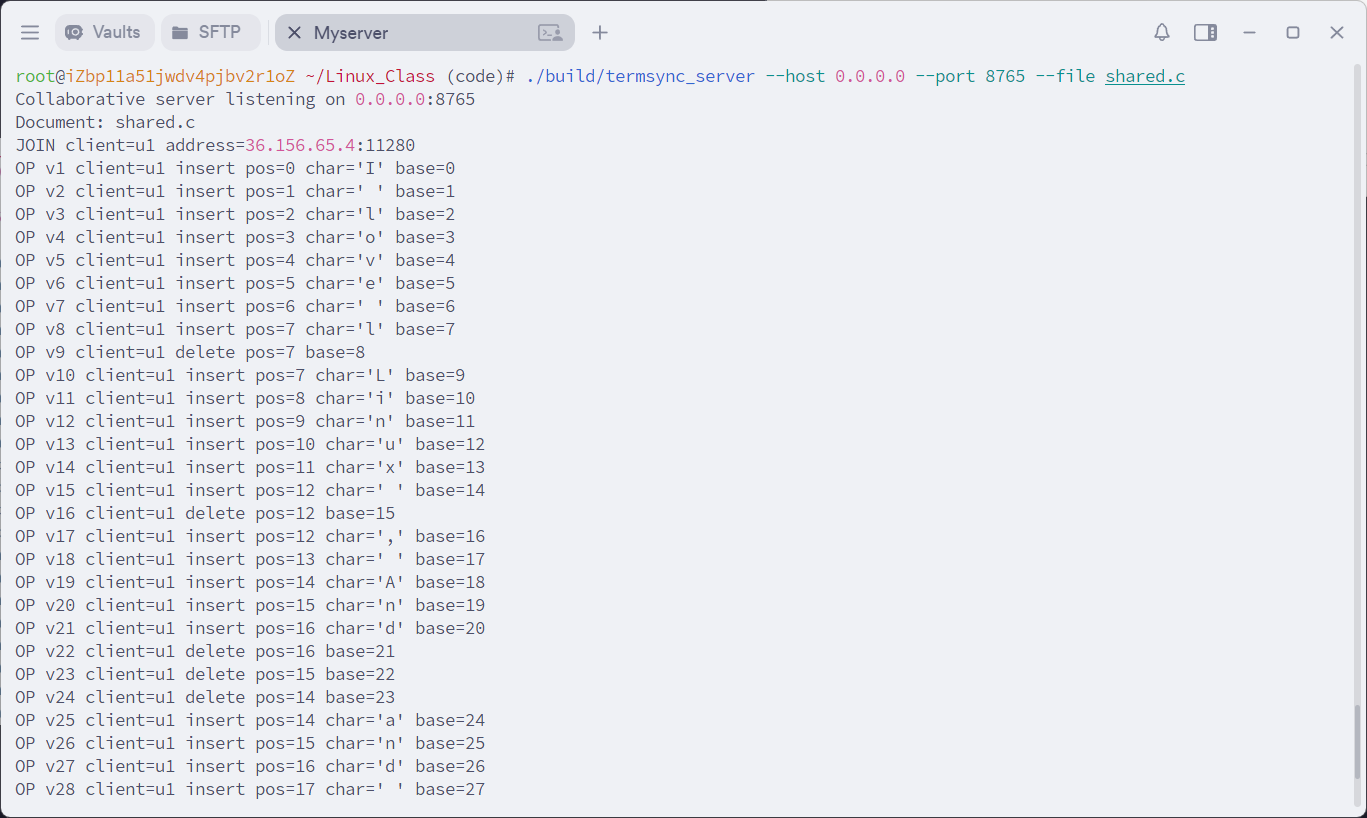
\includegraphics[width=0.8\textwidth]{pic/cowork/服务端运行界面.png}
    \caption{服务端运行界面}
\end{figure}

\begin{figure}[H]
    \centering
    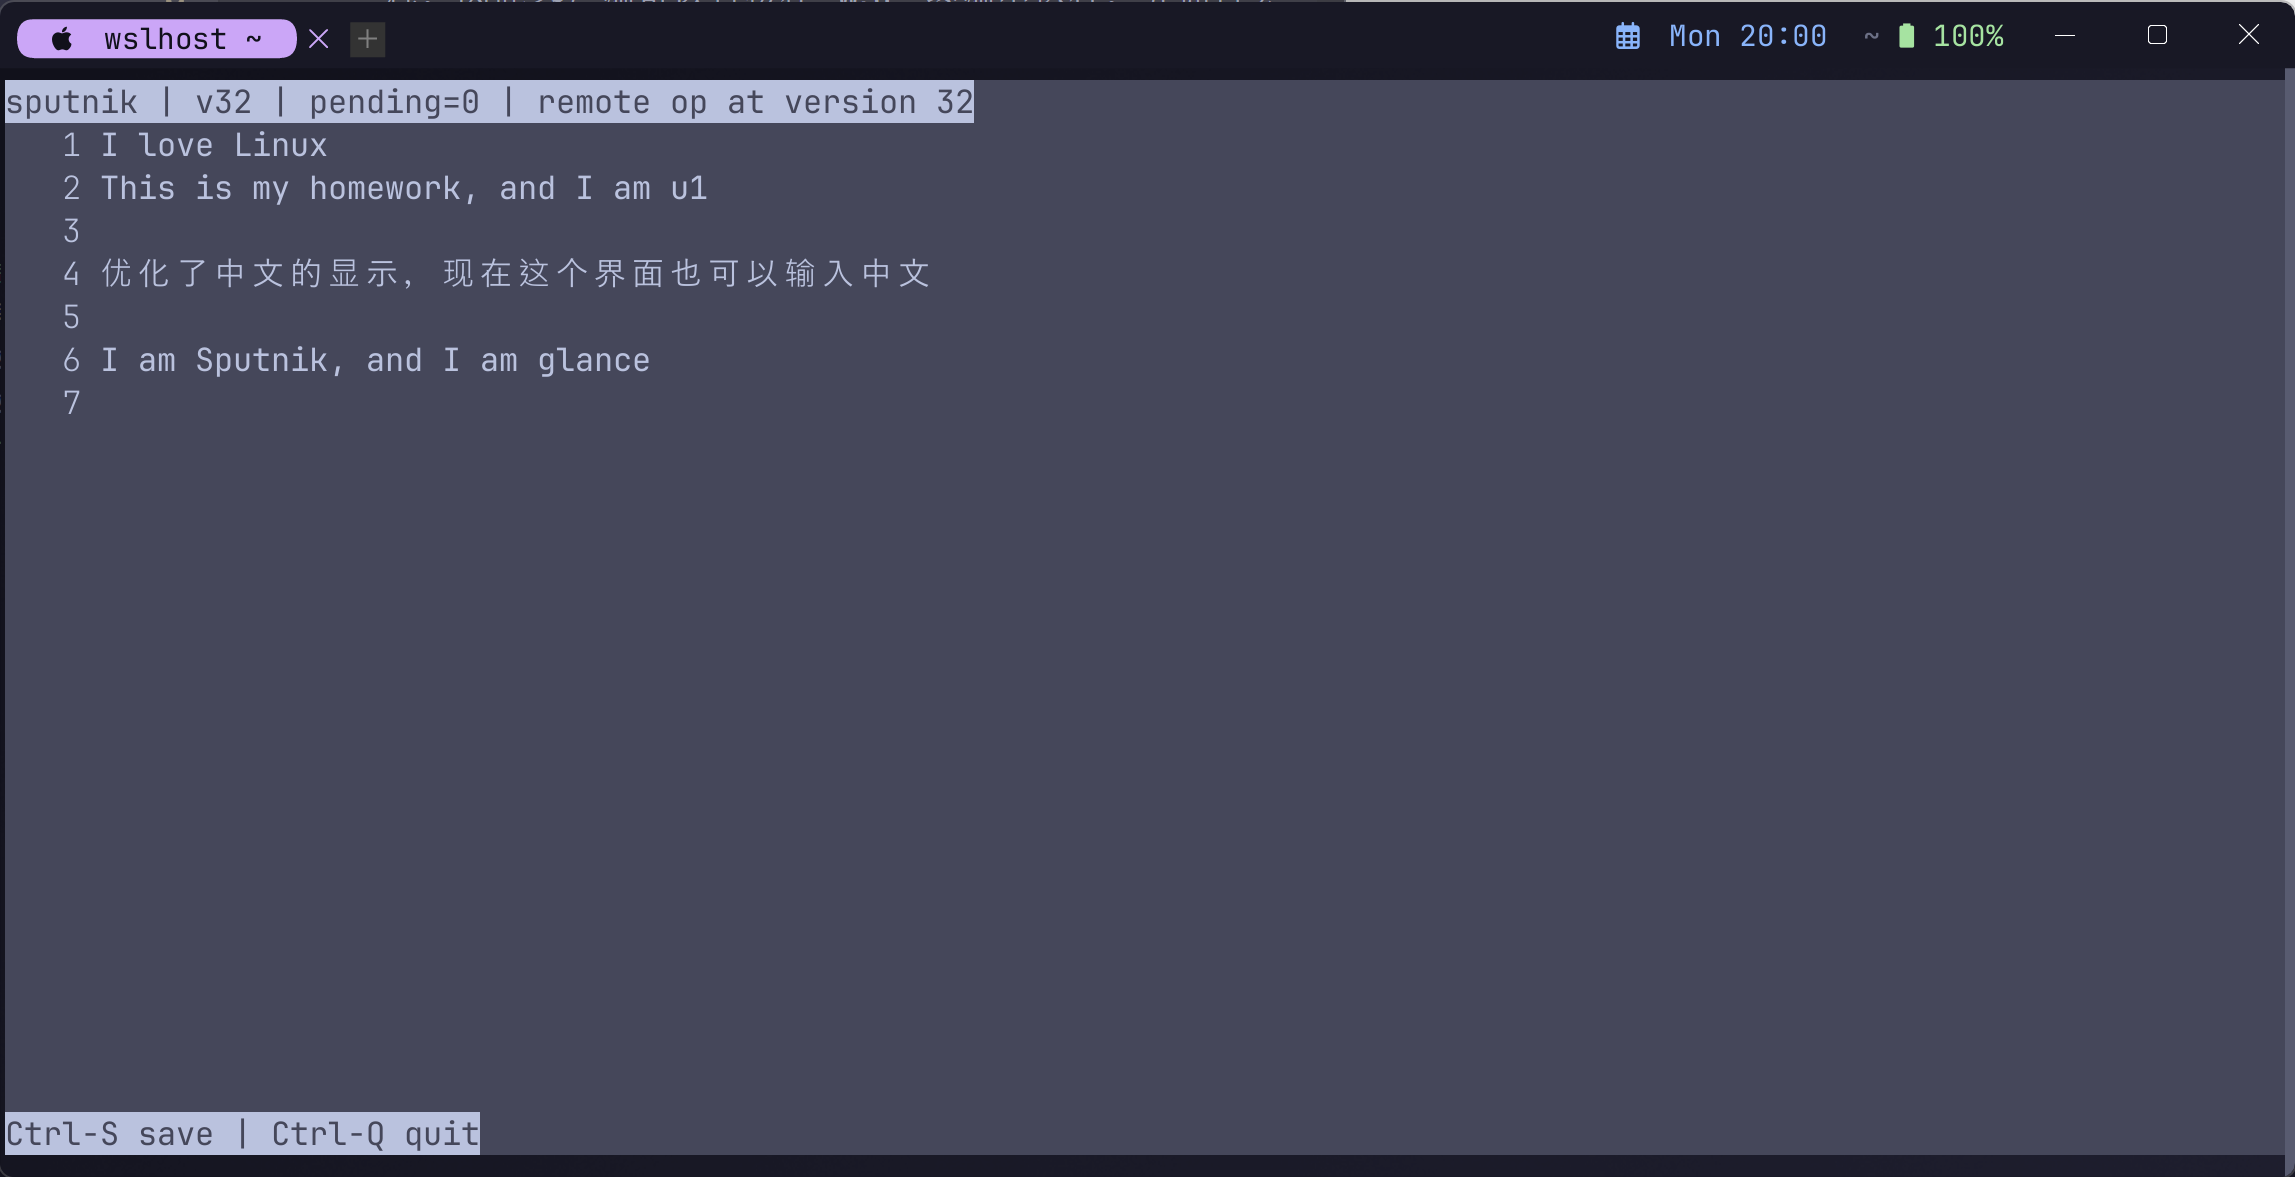
\includegraphics[width=0.82\textwidth]{pic/cowork/客户1连接服务端.png}
    \vspace{0.5em}

    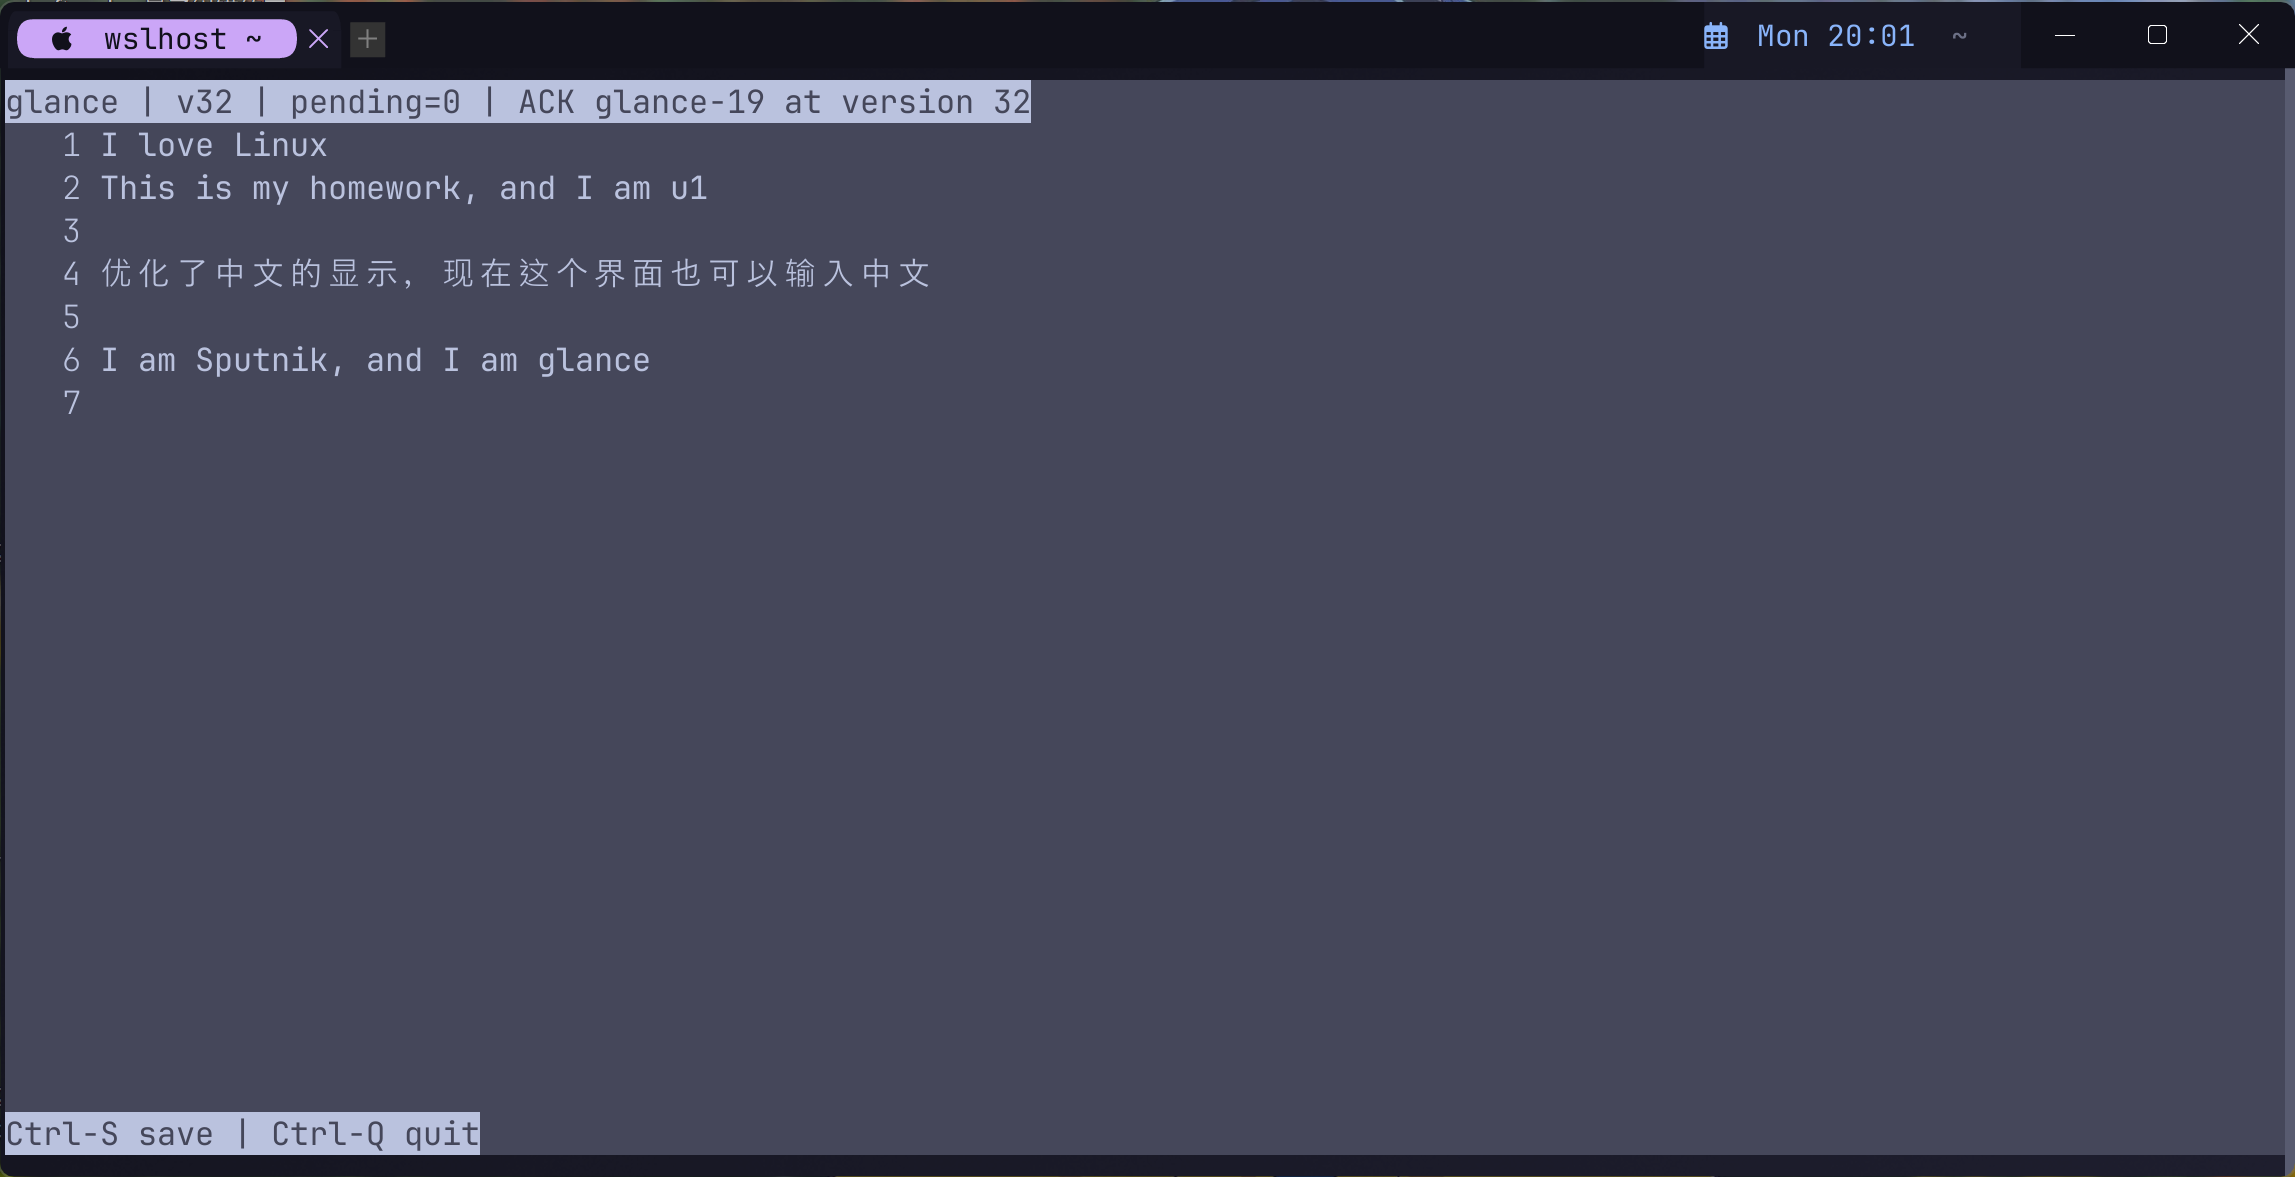
\includegraphics[width=0.82\textwidth]{pic/cowork/客户2连接服务端.png}
    \caption{两个客户端连接服务端}
\end{figure}

前面三张运行截图展示了 TermSync 的基本启动和连接流程。第一张图中，服务端已经在 Linux 服务器上启动并监听指定端口，终端输出中可以看到服务端正在等待客户端接入。后两张图分别展示两个不同客户端通过域名连接到同一个服务端实例，并进入终端编辑界面；这说明服务端可以同时维护多个客户端连接，新加入的客户端也能够获得当前共享文档状态，为后续的同步编辑、广播更新和保存验证提供了运行基础。

项目代码已经开源托管在 GitHub 仓库 \url{https://github.com/glance02/Linux_Class.git} 中。其中，程序实现放在 \cmd{code} 分支，本报告使用 LaTeX 编写、编译完成，其 LaTeX 源码放在 \cmd{master} 分支，便于将可运行代码和课程报告正文分开管理。

\newpage
\subsection{项目背景}

多人协作编辑是一个典型的分布式一致性问题。多个用户可能在同一时间对同一份文本进行修改，如果系统只按照客户端本地光标位置直接修改文档，很容易出现字符位置错乱、删除目标错误、不同客户端内容不一致等问题。例如初始文本为 \cmd{hello world}，一个用户在位置 5 连续插入多个字符，另一个用户仍然基于旧版本请求删除位置 5 的字符。如果服务端不做额外处理，第二个用户想删除的字符和服务端当前文档中的位置就不再对应。

传统协作编辑系统常见的解决方案包括 OT 和 CRDT。本项目选择 OT：每个编辑操作携带自己基于的文档版本，服务端根据该版本之后已经发生的历史操作修正位置，最后将操作应用到当前文档。与更复杂的全客户端协同 OT 不同，本项目采用服务端主导方案，将全局排序和位置变换集中放在服务端，从而使实现更清晰，也更容易验证正确性。

本项目也具有明确的 Linux 课程背景。首先，服务端是一个典型的 TCP 长连接服务，涉及 socket 创建、地址绑定、监听、接受连接和消息收发。其次，每个客户端连接由独立线程处理，多个线程会同时访问共享文档，因此必须使用锁保护临界区。再次，自动保存和日志写入使用独立进程完成，主进程通过队列向工作进程发送快照、保存和日志事件，体现了进程间通信的使用。最后，文件加载、原子写入、备份文件、自动保存文件和编辑日志都体现了 Linux 文件系统编程的基本实践。

此外，终端编辑器本身也与 Linux 使用场景贴合。客户端基于 \cmd{curses} 运行在终端中，支持方向键移动、普通字符输入、回车换行、Backspace 删除、\cmd{Ctrl-S} 保存和 \cmd{Ctrl-Q} 退出。相比网页前端，这种实现更接近 Linux 命令行环境下的工具开发，也便于在服务器和 WSL 中演示。

从项目边界上看，TermSync 更偏向教学型协作编辑器。它重点展示字符级同步、网络通信、并发控制、文件持久化和自动化测试，而不追求语法高亮、代码补全、复杂撤销栈等完整 IDE 功能。这样的取舍使项目能够把主要篇幅集中在 Linux 程序设计课程强调的系统调用、进程线程、终端交互和文件操作上。

\newpage
\subsection{功能描述}

\subsubsection{多人连接与文档同步}

服务端通过 TCP socket 对外提供协作编辑服务。客户端连接后首先发送 \cmd{JOIN} 消息，服务端为其分配或确认 \cmd{client\_id}，随后发送 \cmd{WELCOME} 和完整的 \cmd{DOC\_STATE}。这样新加入的客户端可以立即得到当前文档内容、版本号和历史起始版本。

每个客户端连接由服务端中的一个独立线程处理。线程持续读取该客户端发来的 JSON Lines 消息，并根据消息类型分发到不同处理逻辑。编辑操作使用 \cmd{OP} 消息提交，保存请求使用 \cmd{SAVE} 消息提交，客户端也可以主动发送 \cmd{REQUEST\_DOC} 请求完整文档。

\subsubsection{字符级编辑操作}

项目支持的核心编辑操作是字符级 \cmd{insert} 和 \cmd{delete}。插入操作包含插入位置和单个字符，删除操作包含删除位置。换行符 \cmd{\textbackslash{}n} 被视为普通字符处理，因此多行文本可以自然表示为一个字符串。

客户端终端界面将用户按键转换为这些基础操作。普通可显示字符会生成 \cmd{insert}；回车会生成插入换行符；Backspace 会生成删除光标前一个字符的 \cmd{delete}。客户端本地光标会随着输入移动，但文档内容最终以服务端返回的 ACK 或远程广播为准。

这些操作在代码中的定义集中在代码仓库根目录下的 \cmd{document.py}：\cmd{VALID\_KINDS} 限定操作类型只能是 \cmd{insert}、\cmd{delete} 和 \cmd{noop}，\cmd{Operation} 数据类保存 \cmd{kind}、\cmd{pos}、\cmd{char} 和可选的 \cmd{reason}。客户端在 \cmd{client.py} 的按键处理函数中把普通字符、回车和 Backspace 转换成 \cmd{Operation}，再由 \cmd{client\_state.py} 封装成网络层的 \cmd{OP} 消息。服务端终端上看到的 \cmd{OP v...} 并不是另一种新的操作模型，而是 \cmd{server.py} 中日志格式化函数对服务端事件的可读化输出。

例如一条服务端输出 \cmd{OP v7 client=sputnik insert pos=76 char='S' base=6} 表示：服务端把这次操作确认为全局第 7 个版本，操作来自 \cmd{sputnik} 客户端，最终权威操作是在位置 76 插入字符 \cmd{S}，而客户端提交时基于的是版本 6。换行也按普通字符参与协同编辑，所以回车会显示为 \cmd{char='\textbackslash{}n'}。

字符可以输入英文、数字、符号，也可以输入中文等宽字符。客户端使用 Python 的 \cmd{unicodedata} 模块，通过 \cmd{east\_asian\_width} 判断字符宽度，并提供显示列和字符列之间的转换函数，确保光标移动和文本显示在终端中正确对齐。

\begin{figure}[H]
    \centering
    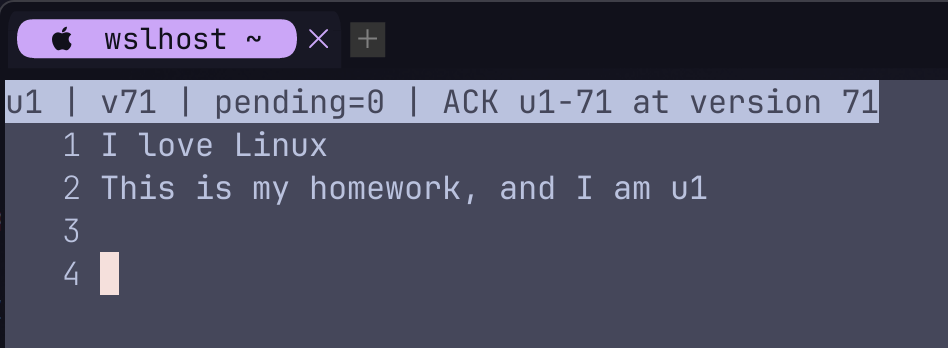
\includegraphics[width=0.8\textwidth]{pic/cowork/服务端u1英文演示.png}
    \caption{服务端英文输入}
\end{figure}

\begin{figure}[H]
    \centering
    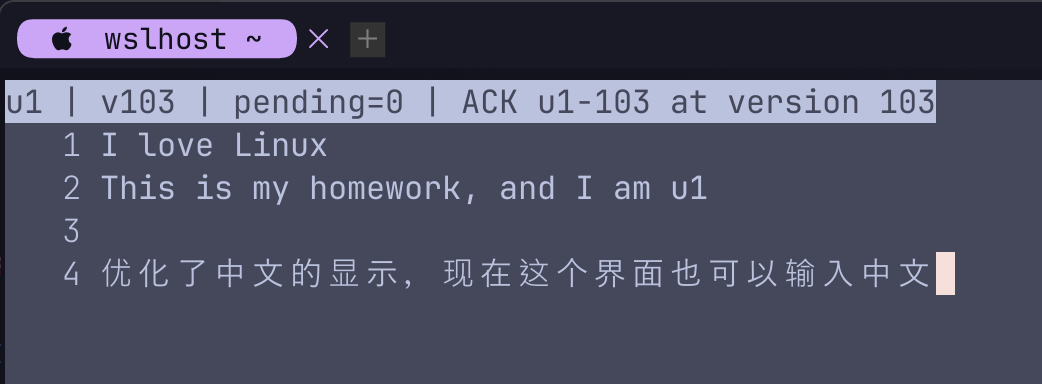
\includegraphics[width=0.8\textwidth]{pic/cowork/服务端u1中文演示.png}
    \caption{服务端中文输入}
\end{figure}


\subsubsection{ACK 驱动的客户端发送队列}

为了避免用户连续快速输入时丢失按键，客户端维护 \cmd{pending\_queue}。每次用户输入产生的操作都会先进入队列。与此同时，客户端同一时刻最多只允许存在一个 \cmd{inflight\_op}，也就是已经发送但尚未收到服务端 ACK 的操作。

当当前操作收到 ACK 后，客户端使用 ACK 中的权威操作更新本地文档，再从队列中取出下一个操作发送。这个设计的好处是客户端不需要实现复杂的 OT 逻辑，只需要维护本地队列和版本号；所有并发冲突都交给服务端处理。

\subsubsection{服务端主导 OT 与全局版本}

服务端的文档对象维护当前文本、当前版本号、有限历史记录和文档锁。所有编辑操作只有进入文档锁保护的临界区后，才会被分配新的 \cmd{server\_version}。这个版本号既表示文档版本，也表示操作在全局历史中的顺序。

当客户端提交的 \cmd{base\_version} 落后于服务端当前版本时，服务端会从历史记录中取出该版本之后的所有操作，逐条对客户端操作进行位置变换。例如历史中已经发生过一次插入，那么位于插入点之后的操作位置需要右移；如果两个删除操作删除同一个字符，后到达的删除会被转换为 \cmd{noop}。

\subsubsection{保存、自动保存与编辑日志}

服务端启动时会加载指定文档文件。如果文件不存在，则以空文档开始。成功处理编辑操作后，服务端会把最新快照发送给自动保存进程。自动保存进程定期写入 \cmd{.autosave} 文件，避免每次按键都直接触发磁盘写入。

用户在客户端按下 \cmd{Ctrl-S} 后，客户端发送 \cmd{SAVE} 消息。服务端收到后将当前快照投递给自动保存进程，由工作进程写入正式文件。为了降低误覆盖风险，正式保存前会生成 \cmd{.bak} 备份文件。同时，服务端会记录加入、离开、操作、自动保存和手动保存等事件，形成 JSON Lines 格式的编辑日志。

\begin{figure}[H]
    \centering
    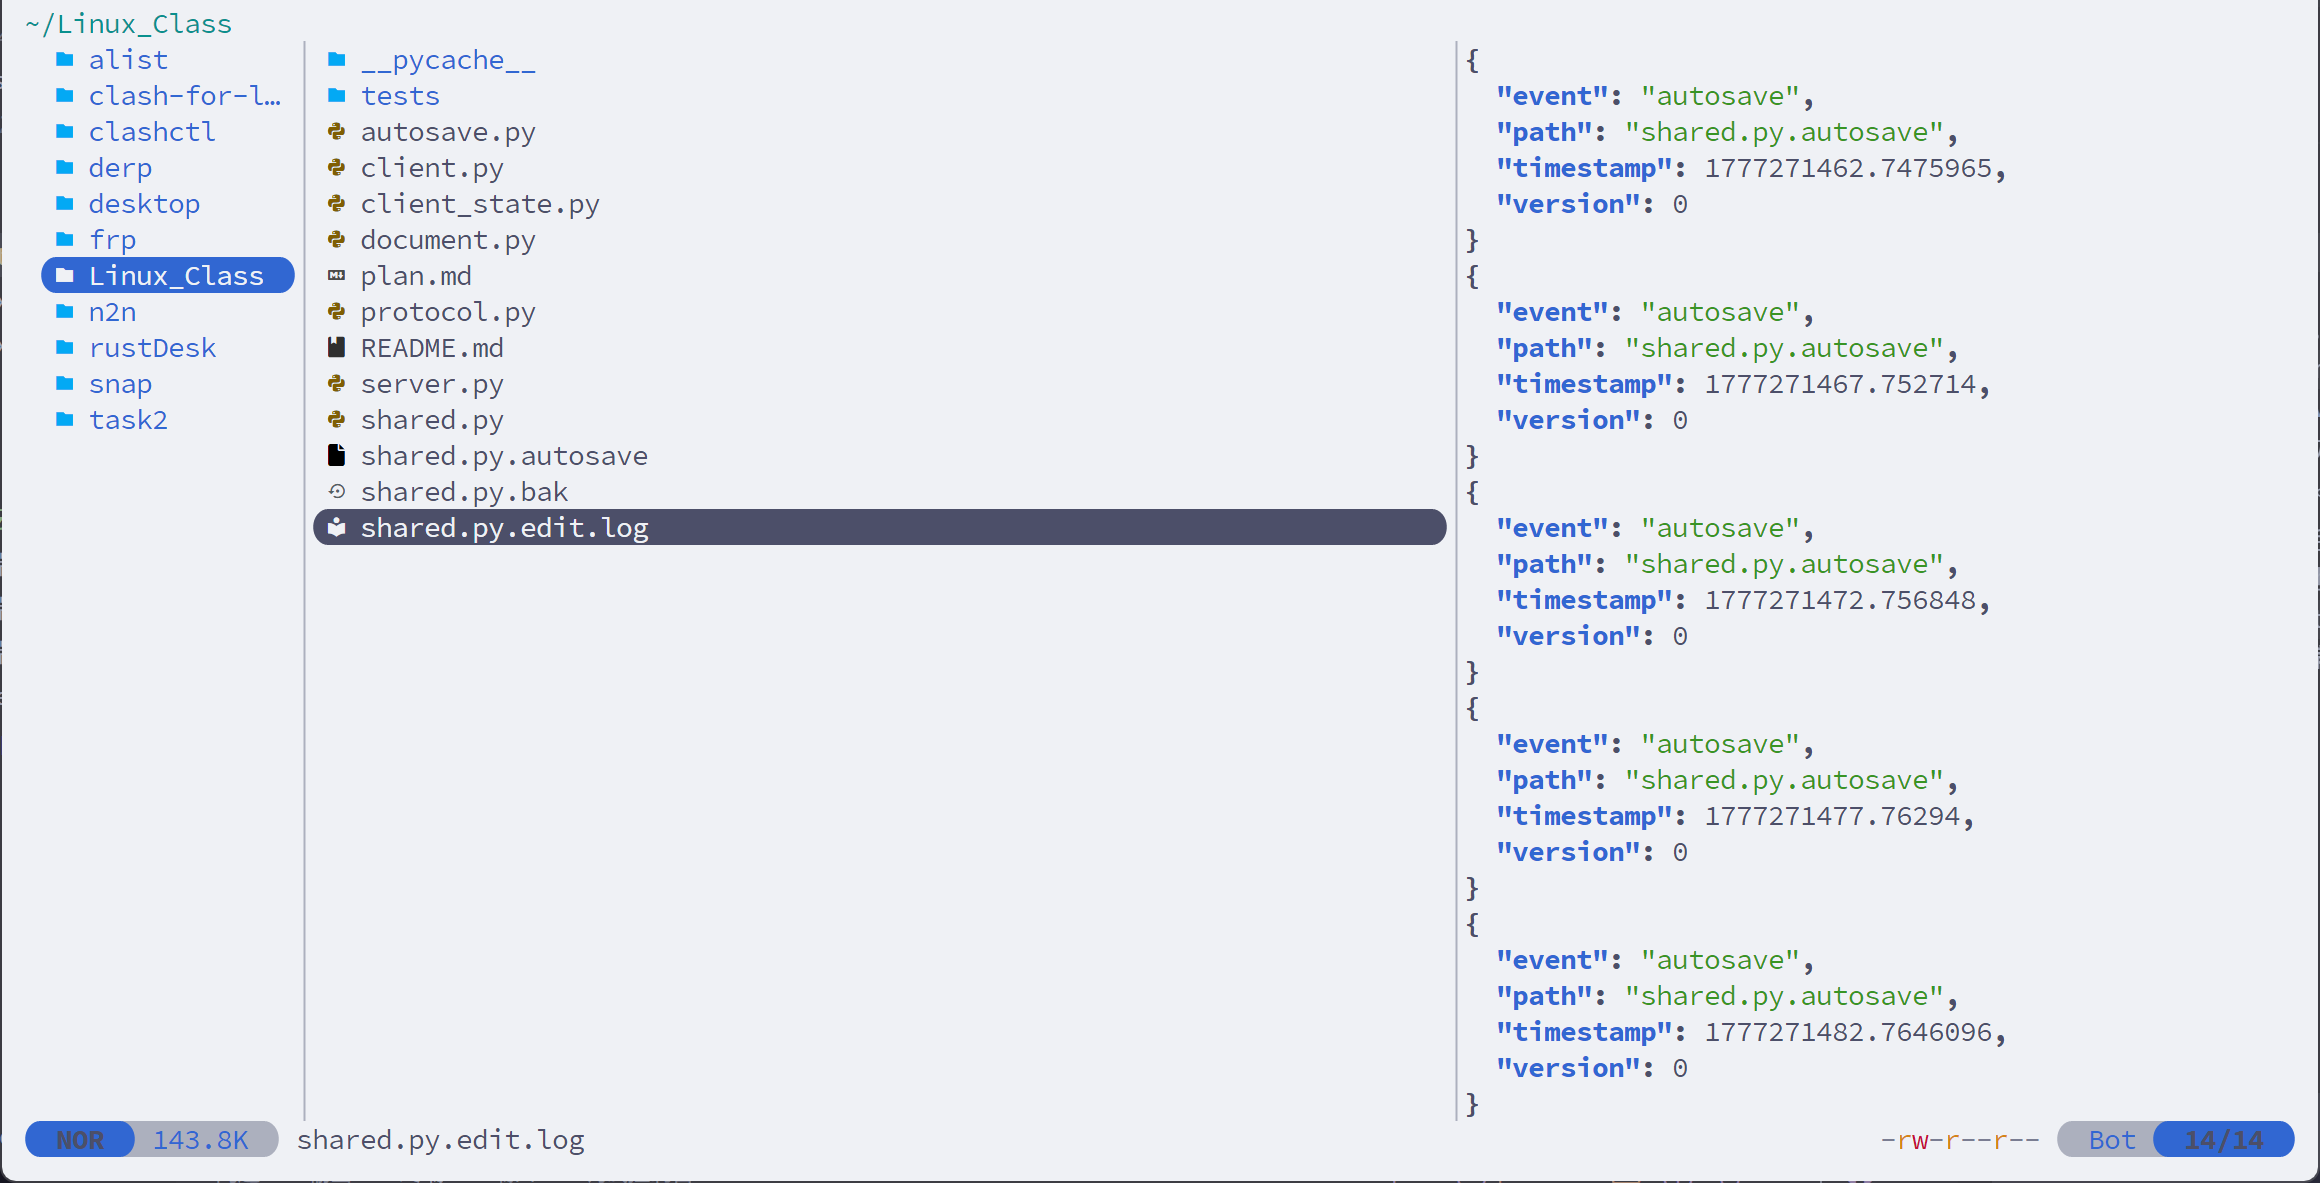
\includegraphics[width=0.8\textwidth]{pic/cowork/服务日志图片.png}
    \caption{服务端编辑日志与自动保存记录}
    \label{fig:log and bak}
\end{figure}

图~\ref{fig:log and bak}中展示了服务端运行目录中的保存产物和编辑日志。左侧可以看到正式文档 \cmd{shared.py}、自动保存文件 \cmd{shared.py.autosave}、备份文件 \cmd{shared.py.bak} 以及编辑日志 \cmd{shared.py.edit.log} 同时存在，说明服务端把文档内容、自动保存快照、覆盖前备份和事件记录分开管理。右侧打开的日志文件由多条 JSON 事件组成，每条记录包含 \cmd{event}、\cmd{path}、\cmd{timestamp} 和 \cmd{version} 等字段；其中 \cmd{autosave} 事件表示自动保存进程已经按固定间隔将当前快照写入 \cmd{.autosave} 文件。后续发生手动保存或编辑操作时，同一日志文件还会继续追加 \cmd{manual\_save}、\cmd{operation} 等记录，用于追踪服务端文档状态的变化过程。

\subsubsection{历史裁剪与重同步}

为了避免服务端无限保存历史操作，文档对象使用有限长度的历史记录，默认保留最近 1000 条操作。服务端同时维护 \cmd{history\_start\_version}，表示当前历史仍然能够支持 OT 变换的最早基准版本。

如果某个客户端提交的 \cmd{base\_version} 已经过旧，服务端无法可靠地根据有限历史进行变换，此时会返回 \cmd{RESYNC\_REQUIRED}，并发送完整的 \cmd{DOC\_STATE}。客户端收到后清空当前未确认操作，并请求或接受完整文档，从而恢复到服务端权威状态。

\newpage
\subsection{设计思路}

\subsubsection{总体架构}

项目整体采用客户端--服务端架构。客户端只负责终端界面、键盘输入、发送队列和接收服务端消息；服务端负责网络连接管理、文档权威状态、操作排序、OT 变换、广播、保存和日志。这样划分后，系统中最关键的一致性逻辑集中在服务端，便于通过单元测试验证。

系统主要模块如下：

\begin{itemize}
  \item \cmd{protocol.py}：封装 JSON Lines 消息的编码、解码和 socket 收发。
  \item \cmd{document.py}：实现权威文档、操作模型、OT 变换、版本历史和重同步判断。
  \item \cmd{server.py}：实现 TCP 服务端、客户端线程、消息分发、广播和自动保存进程管理。
  \item \cmd{client\_state.py}：实现客户端同步状态、待发送队列、ACK 处理和远程操作应用。
  \item \cmd{client.py}：实现 curses 终端界面、光标移动、按键处理和网络连接。
  \item \cmd{autosave.py}：实现自动保存、手动保存、备份和日志写入工作进程。
  \item \cmd{tests/}：包含文档、客户端状态、服务端输出和自动保存相关单元测试。
\end{itemize}

为了更直观地说明各个模块之间的关系，我将系统划分为界面层、网络协议层、同步控制层、权威文档层和持久化层。客户端侧主要覆盖界面层、发送队列和接收消息处理；服务端侧则集中承担权威文档、全局顺序、操作变换、广播和落盘。这样的分层使每一部分都能对应到一个比较明确的 Linux 程序设计主题：终端界面对应 \cmd{curses}，网络协议对应 \cmd{socket}，并发处理对应 \cmd{threading}，自动保存对应 \cmd{multiprocessing} 和文件系统操作。

\begin{figure}[H]
    \centering
    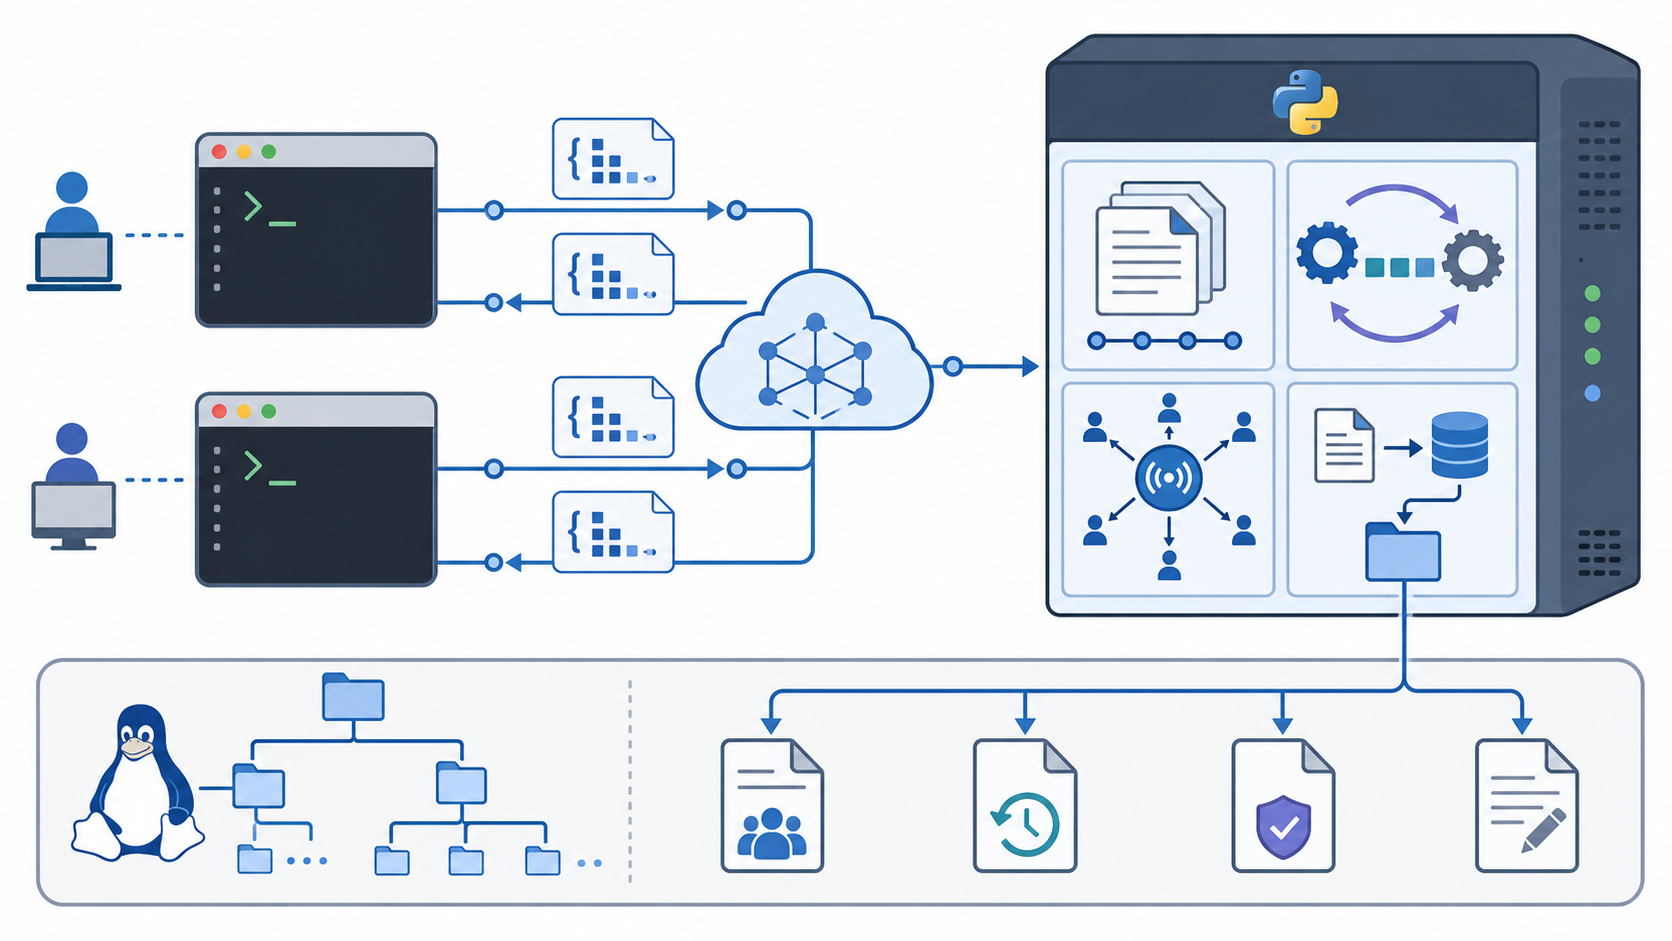
\includegraphics[width=0.9\textwidth]{pic/cowork/TermSync总体架构图.png}
    \caption{TermSync 总体架构示意图}
\end{figure}

图中的两个客户端并不是两个独立文档副本的最终裁判，而只是用户输入和显示结果的入口。真正决定文档内容的是服务端内部的权威文档对象。客户端把每一次按键转换为操作并提交给服务端，服务端在统一版本序列中确认操作后，再把结果返回给提交者并广播给其他客户端。保存进程则作为旁路模块接收文档快照，负责把共享文档、自动保存文件、备份文件和日志文件写入 Linux 文件系统。


从运行过程看，用户在终端中输入一个字符，实际上会经过“按键事件、客户端操作对象、网络消息、服务端临界区、权威操作、ACK、远程广播、界面刷新”这一整条链路。如果把所有逻辑都放到一个文件中，虽然短期内也能运行，但很难解释哪个部分负责一致性、哪个部分负责显示、哪个部分负责保存。现在的模块拆分让项目更适合作为课程报告展示：每个文件都对应一种清晰的系统能力，阅读代码时也能顺着数据流从客户端走到服务端。

\subsubsection{网络协议设计}

网络协议采用 JSON Lines，即每一条消息都是一个 JSON 对象，并以换行符结束。这种格式便于调试，也便于处理 TCP 粘包和拆包问题。接收端维护字节缓冲区，持续读取 socket 数据，直到遇到换行符后再解码一条完整消息。

典型的编辑操作消息包含消息类型、客户端标识、操作编号、基准版本和操作内容。例如：

\begin{minted}{json}
{
    "type": "OP",
    "client_id": "u1",
    "op_id": "u1-12",
    "base_version": 8,
    "op": {
        "kind": "insert",
        "pos": 5,
        "char": "a"
    }
}
\end{minted}

服务端处理成功后会给提交者返回 \cmd{ACK}，并向其他客户端广播 \cmd{REMOTE\_OP}。这两类消息都携带服务端确认后的 \cmd{server\_version} 和变换后的权威操作。客户端只应用服务端确认的操作，而不把本地预测结果直接作为最终文档。

协议层的一个重要原则是消息要足够简单，便于在终端和日志中直接观察。每条消息都是一行 JSON，服务端输出日志时也会尽量把关键字段显示为可读文本。这样在调试时可以同时观察客户端界面、服务端终端和日志文件，判断某个字符是否被发送、是否被服务端确认、是否被其他客户端接收。

\begin{figure}[H]
    \centering
    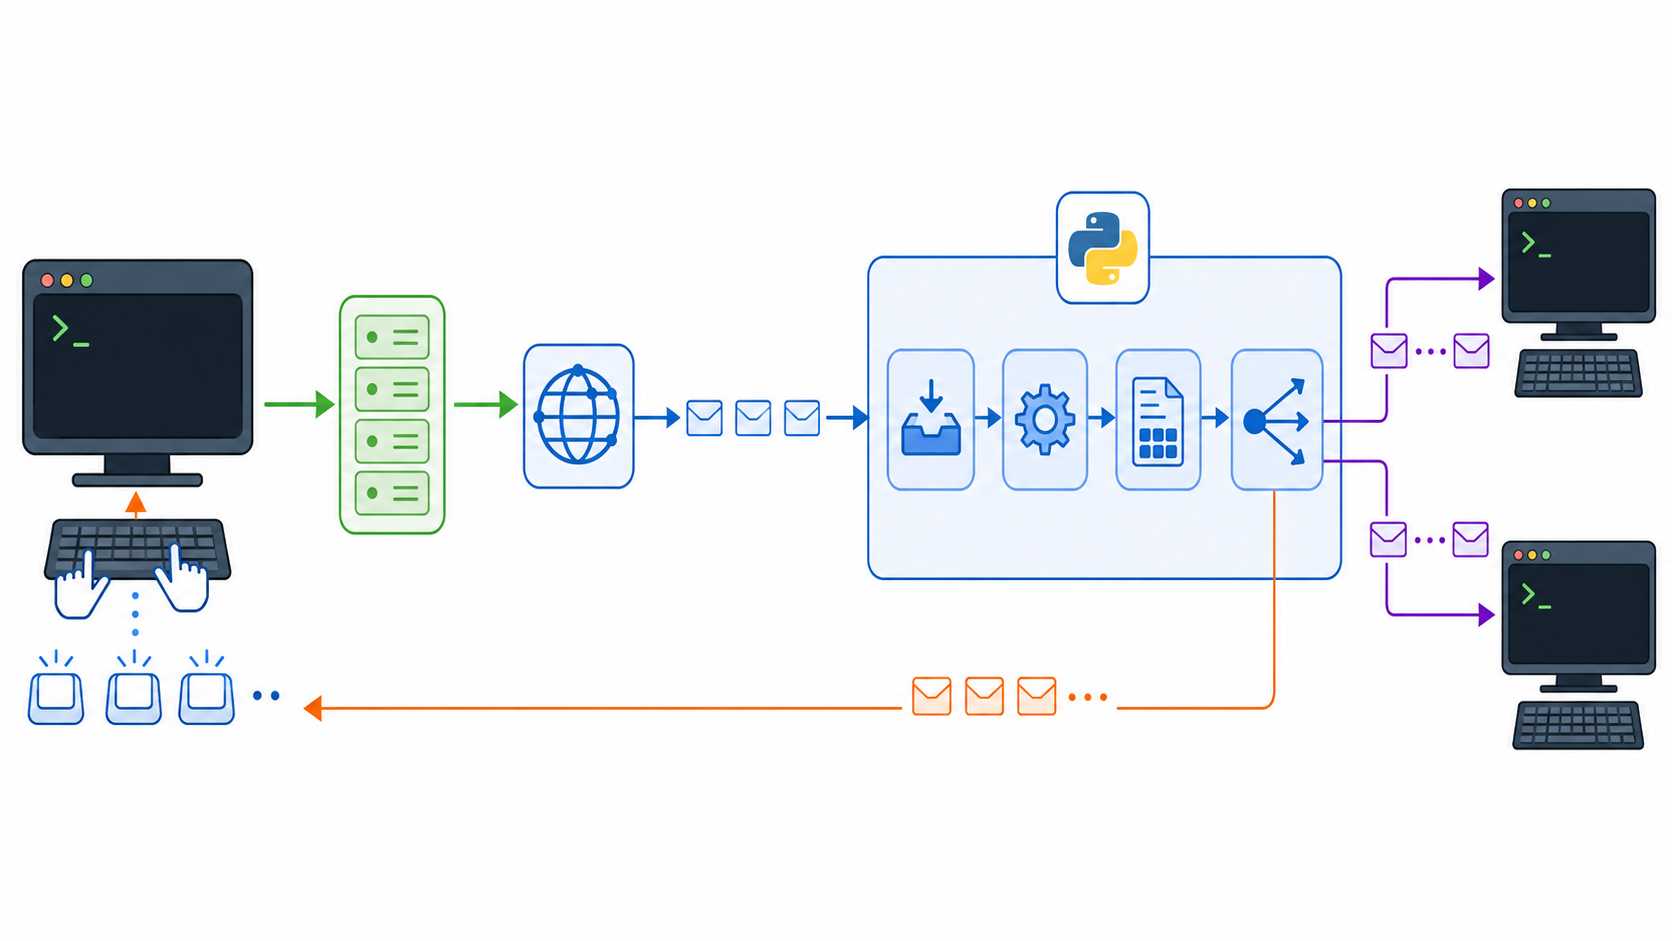
\includegraphics[width=0.9\textwidth]{pic/cowork/客户端到服务端的数据流图.png}
    \caption{客户端与服务端消息流示意图}
\end{figure}

图中展示了从键盘输入到远程同步的完整消息流。客户端不会直接把本地显示结果当成最终状态，而是把操作提交给服务端等待确认。服务端收到操作后，先在文档模型中完成版本检查和 OT 变换，再生成两类结果：一类是发回提交者的 \cmd{ACK}，用于确认队列中的当前操作；另一类是发给其他客户端的 \cmd{REMOTE\_OP}，用于同步远程修改。这样可以保证不同客户端虽然接收消息的时间不同，但最终都以相同的服务端版本序列为准。


在这个协议中，\cmd{op\_id} 和 \cmd{server\_version} 的含义不同。\cmd{op\_id} 由客户端生成，用来识别“我刚才发出去的是哪一次按键”；\cmd{server\_version} 由服务端生成，用来表示“这次操作在全局文档历史中的顺序”。前者解决客户端队列匹配问题，后者解决多客户端一致性问题。把这两个编号分开，可以避免把本地操作顺序误当作全局操作顺序。

\subsubsection{文档锁与全局顺序}

多客户端并发编辑时，服务端会有多个线程几乎同时收到 \cmd{OP} 消息。如果每个线程直接修改文档，就会出现竞争条件。因此文档对象内部使用可重入锁保护临界区。只有持有文档锁的线程才能检查版本、执行 OT、分配版本号、修改文本和写入历史。

这里的设计重点是：服务端不是按照客户端时间戳决定顺序，也不是按照网络包发出时间决定顺序，而是按照操作进入文档临界区的顺序决定全局顺序。进入临界区后分配的递增 \cmd{server\_version} 就是最终权威顺序。这样可以避免分布式时间带来的不确定性。

另一方面，socket 发送和广播不能放在文档锁内部。如果某个客户端网络很慢，持锁发送会导致其他客户端的编辑操作无法进入临界区，扩大阻塞范围。因此服务端在文档锁内只生成 ACK 和广播消息，返回后再执行 socket I/O。

\subsubsection{OT 位置变换规则}

本项目使用字符级 OT，因此变换规则集中在位置调整上。当前操作会依次与它的 \cmd{base\_version} 之后已经发生的历史操作进行比较：

\begin{itemize}
  \item 历史操作是插入时，当前插入或删除如果位于该插入位置之后或相同位置，就需要右移一位。
  \item 历史操作是删除时，当前插入如果位于删除位置之后，需要左移一位。
  \item 历史操作是删除时，当前删除如果位于删除位置之后，需要左移一位。
  \item 两个删除操作删除同一位置时，后一个删除变为 \cmd{noop}，因为目标字符已经被删除。
\end{itemize}

服务端还会对最终操作做规范化处理，例如插入位置会被限制在文档长度范围内，越界删除会变为 \cmd{noop}。这能提高协议容错性，避免异常客户端破坏服务端文档状态。

\begin{figure}[H]
    \centering
    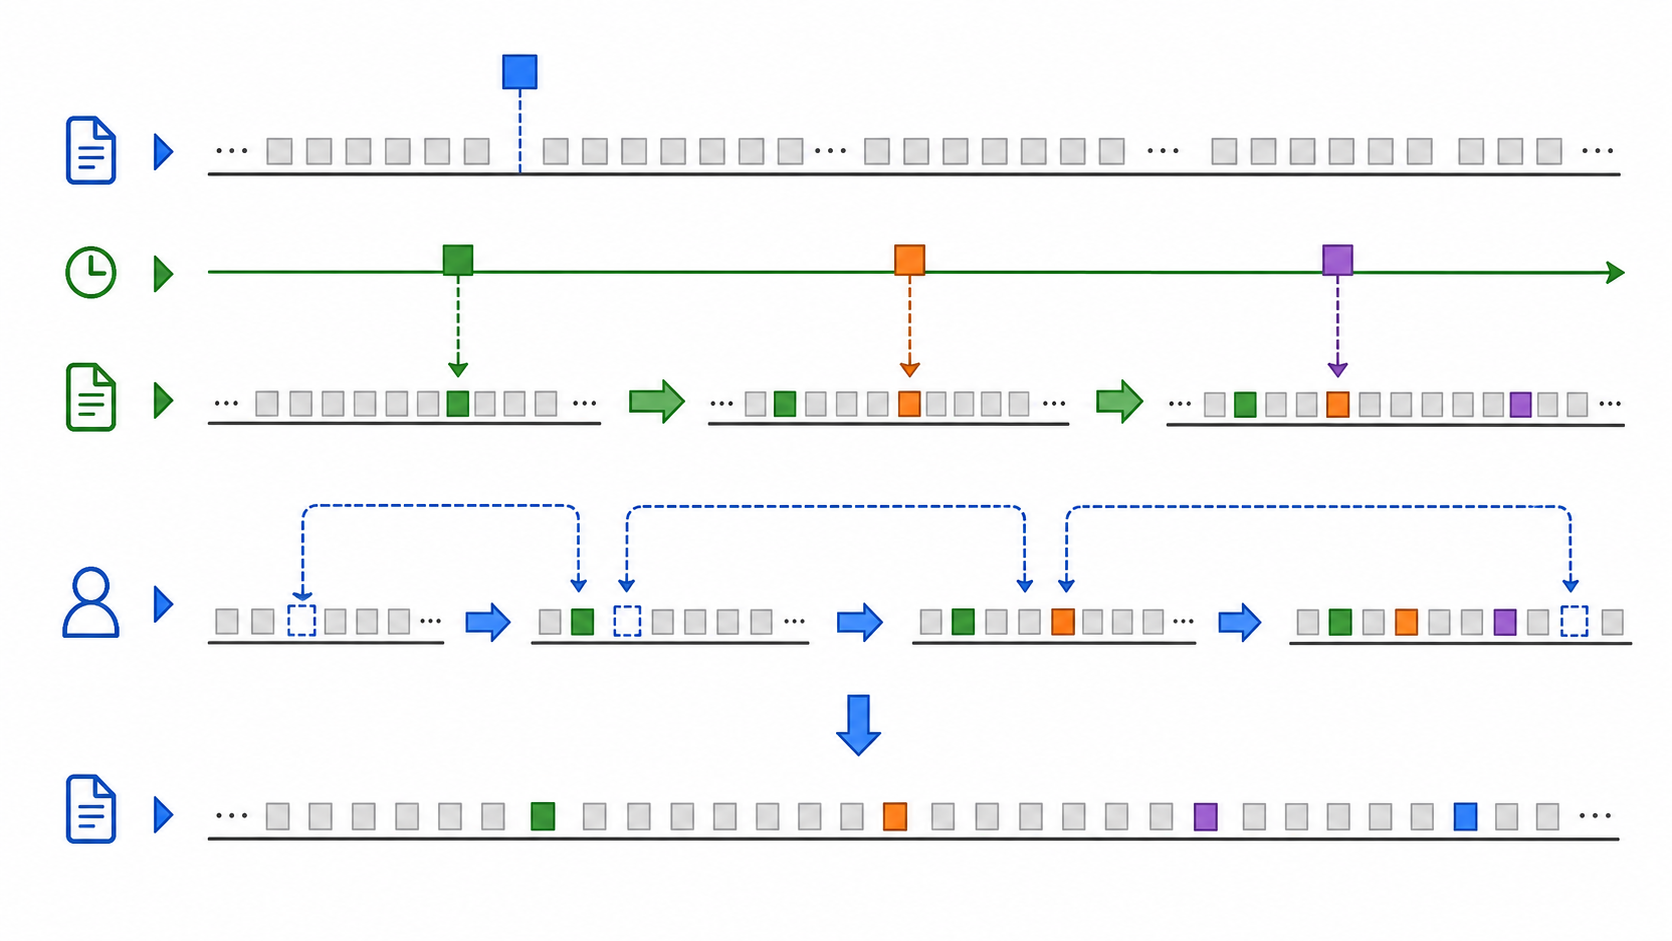
\includegraphics[width=0.88\textwidth]{pic/cowork/OT位置变换示意图.png}
    \caption{OT 位置变换过程示意图}
\end{figure}

图中的核心思想是：客户端提交的位置并不一定能直接用于当前服务端文本，因为这个位置可能基于旧版本。服务端需要把该操作与历史中已经确认的操作逐个比较，把旧位置转换到当前版本。这个过程并不是简单地按时间戳覆盖，而是根据插入、删除对字符索引造成的影响进行位置修正。

\begin{table}[H]
    \centering
    \caption{典型 OT 变换场景}
    \small
    \begin{tabular}{p{0.20\textwidth} p{0.24\textwidth} p{0.24\textwidth} p{0.20\textwidth}}
        \toprule
        场景 & 历史操作 & 当前旧版本操作 & 变换结果 \\
        \midrule
        历史先插入 & 在位置 5 插入字符 & 在位置 8 插入字符 & 当前操作位置右移到 9 \\
        历史先删除 & 删除位置 5 的字符 & 在位置 8 插入字符 & 当前操作位置左移到 7 \\
        删除同一字符 & 删除位置 5 的字符 & 也删除位置 5 的字符 & 当前操作变为 \cmd{noop} \\
        尾部插入 & 在文档末尾插入字符 & 在较旧末尾继续插入 & 根据历史插入次数整体右移 \\
        越界删除 & 文档已变短 & 删除一个不存在的位置 & 服务端规范化为 \cmd{noop} \\
        \bottomrule
    \end{tabular}
\end{table}

例如两个客户端都基于版本 0 编辑同一个位置，客户端 A 先到达服务端并在位置 10 插入字符，服务端将其确认成版本 1。客户端 B 的操作随后到达时，仍然携带 \cmd{base\_version=0}。如果 B 也要在位置 10 附近插入字符，服务端就会根据版本 1 的历史插入把 B 的位置向后调整，保证两个字符都被保留。这个例子说明 OT 的目标不是让所有客户端“同时发生”的操作互相覆盖，而是在服务端确定的全局顺序下尽量保留每个用户的编辑意图。

本项目的 OT 实现刻意保持字符级粒度，没有引入复杂的富文本属性、区间操作或多光标语义。这样做的好处是规则可以通过单元测试直接验证，也便于在报告中解释清楚；不足是快速输入长文本时会产生较多操作。对于课程项目而言，字符级 OT 更能突出位置变换、历史记录和版本一致性的核心问题。

\subsubsection{客户端状态机}

客户端状态机的核心是 \cmd{pending\_queue} 和 \cmd{inflight\_op}。用户输入不会直接阻塞等待网络响应，而是先进入队列；发送函数只在当前没有未确认操作时才取出队首并发送。每条操作发送时会记录当前客户端已知版本作为 \cmd{base\_version}。

客户端收到 ACK 后，会检查 ACK 的 \cmd{op\_id} 是否对应当前 \cmd{inflight\_op}。如果匹配，就应用服务端返回的权威操作，更新版本号，清空 \cmd{inflight\_op}，再继续发送队列中的下一个操作。客户端收到远程操作时，也会检查版本是否连续。如果发现远程版本跳跃，说明中间可能漏收消息，于是请求完整文档。

\subsubsection{自动保存进程}

自动保存和日志写入被放在独立进程中完成。主服务端进程处理网络和文档同步，自动保存进程负责磁盘 I/O。二者通过 \cmd{multiprocessing.Queue} 传递事件。服务端每处理完一次成功编辑，就发送最新快照；工作进程只保留最新内容，并按固定间隔写入 \cmd{.autosave} 文件。

手动保存时，服务端向队列发送 \cmd{SAVE\_NOW} 事件。工作进程先复制旧文件作为 \cmd{.bak} 备份，再使用临时文件替换的方式写入正式文件。这样既体现了进程间通信，也减少了主服务端在网络请求处理过程中直接进行磁盘写入的时间。

\begin{figure}[H]
    \centering
    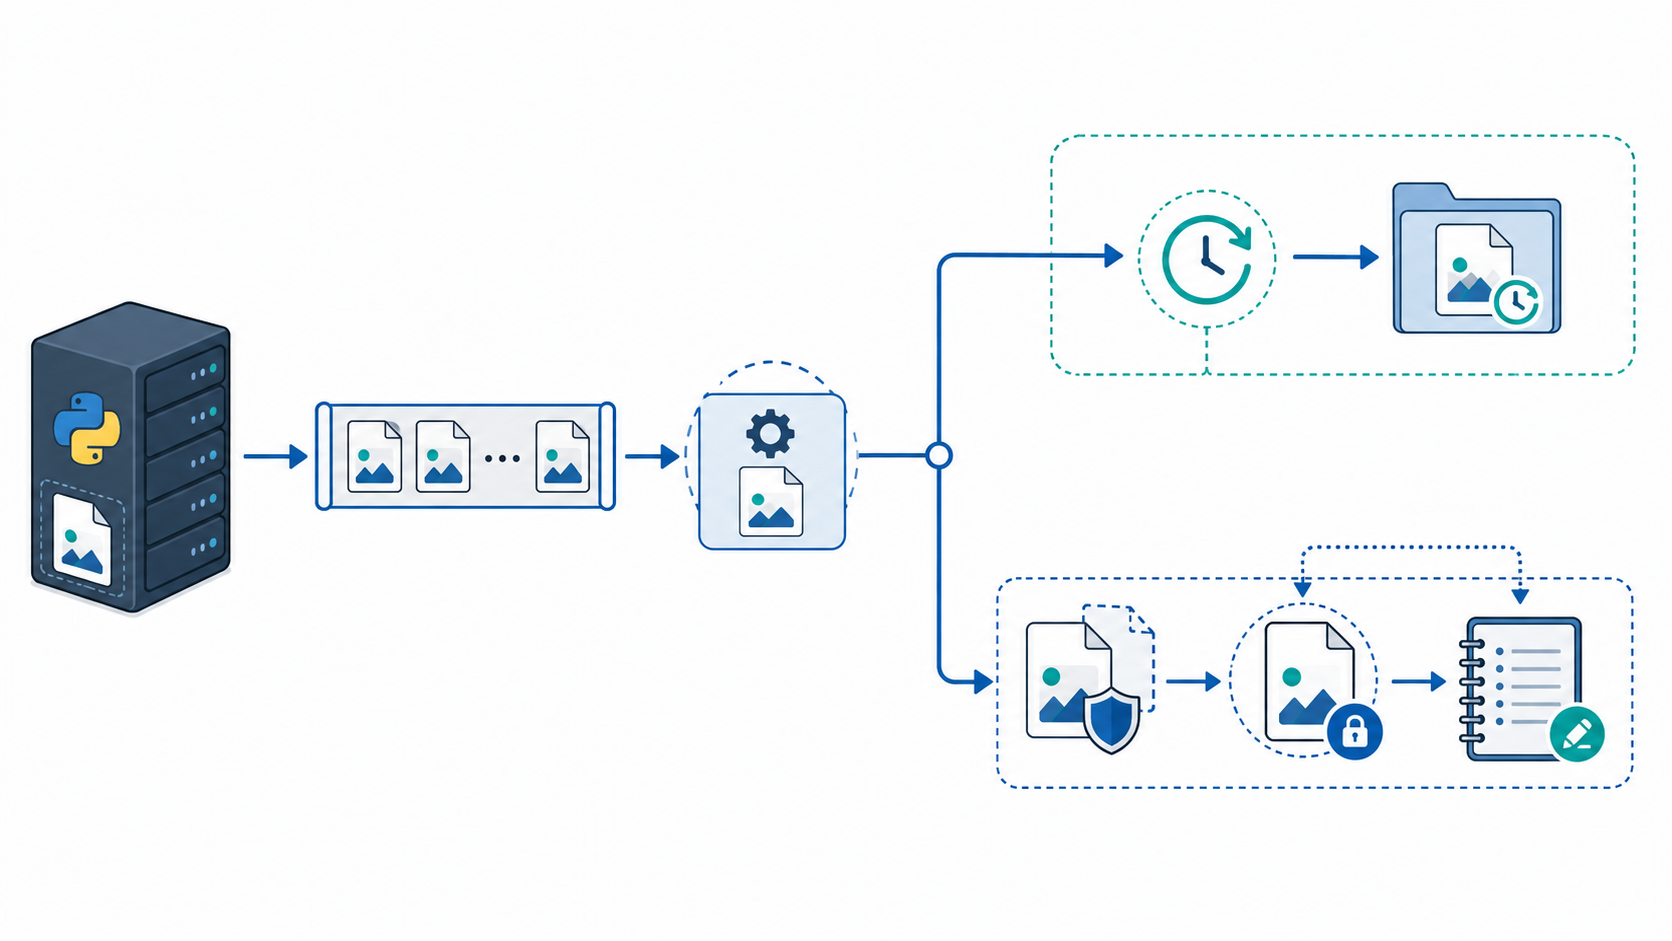
\includegraphics[width=0.88\textwidth]{pic/cowork/自动保存与备份流程图.png}
    \caption{自动保存与备份流程示意图}
\end{figure}

自动保存流程的设计重点在于把“编辑同步”和“磁盘写入”分开。服务端主线程和客户端处理线程负责响应网络事件，尽量不要因为磁盘 I/O 而阻塞；保存进程则通过队列接收最新快照，按照固定间隔写入 \cmd{.autosave} 文件。手动保存时，保存进程会先备份旧文件，再写入正式文件，这样即使用户在演示时误保存，也仍然可以从 \cmd{.bak} 中恢复上一个正式版本。


这种设计也体现了 Linux 程序中常见的可靠写入思路：先把新内容写入临时文件，再使用替换操作更新目标文件。相比直接打开正式文件覆盖写入，临时文件替换可以降低程序中断、系统异常或磁盘写入失败造成文件损坏的概率。虽然本项目不是生产级编辑器，但这个保存流程已经比简单的 \cmd{open(..., "w")} 更可靠，也更符合课程中关于文件系统操作和异常处理的要求。

\newpage
\subsection{测试与验证}

\subsubsection{单元测试}

项目使用 Python 标准库 \cmd{unittest} 进行自动化测试。实际运行时，可以在 Linux 服务器克隆 \cmd{code} 分支后，进入克隆得到的代码仓库根目录执行测试命令：

\begin{minted}{bash}
python3 -m unittest discover -s tests -v
\end{minted}

本地执行结果显示，共运行 17 个测试用例，所有测试均通过，输出结尾为 \cmd{Ran 17 tests ... OK}。

测试覆盖的关键场景包括：

\begin{itemize}
  \item \cmd{server\_version} 严格递增，保证服务端全局顺序明确。
  \item 基于旧版本的删除操作经过历史插入变换后，删除位置正确右移。
  \item 两个客户端删除同一字符时，后到达的删除被转换为 \cmd{noop}。
  \item 历史记录裁剪后，过旧 \cmd{base\_version} 会触发重同步响应，并返回完整文档状态。
  \item 客户端连续输入时，只发送一个未确认操作，后续操作留在 \cmd{pending\_queue} 中等待 ACK。
  \item 客户端发现远程版本不连续时，会发送 \cmd{REQUEST\_DOC} 请求完整文档。
  \item 中文字符可以被插入，终端显示宽度辅助函数能正确处理宽字符。
  \item 手动保存时会在覆盖正式文件前生成备份文件。
\end{itemize}

\begin{figure}[H]
    \centering
    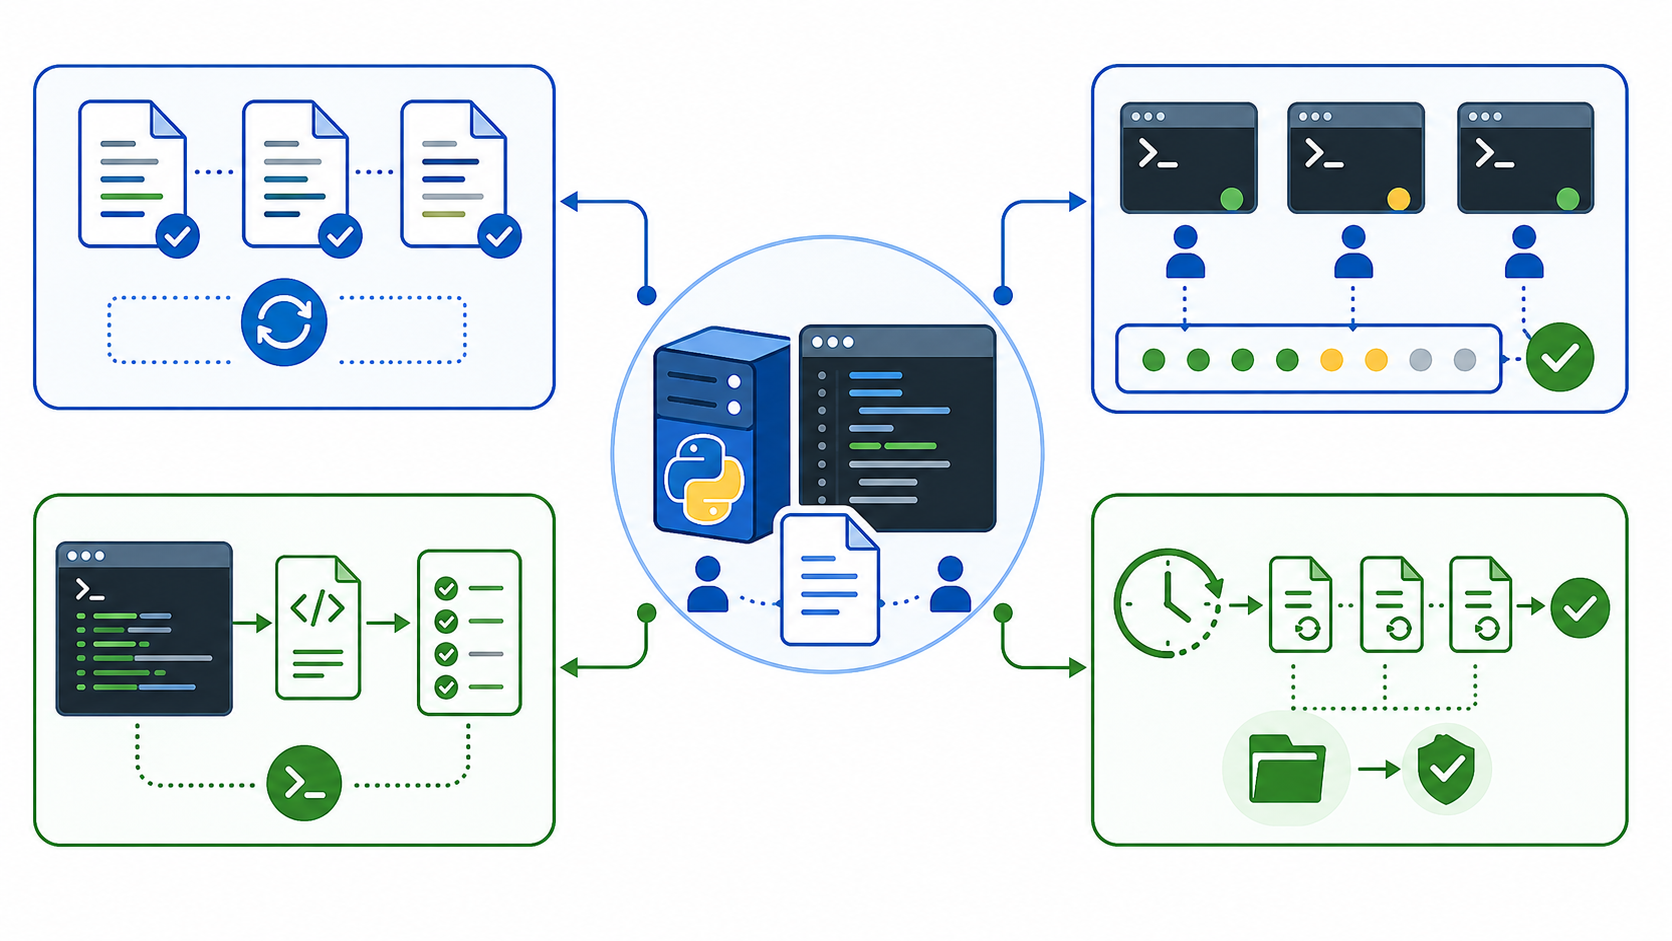
\includegraphics[width=0.88\textwidth]{pic/cowork/测试验证覆盖图.png}
    \caption{测试验证覆盖关系示意图}
\end{figure}

测试验证并不是只为了得到一个 \cmd{OK}，更重要的是把项目中最容易出错的状态变化固定下来。TermSync 的风险点主要集中在三个方面：第一，多线程同时修改文档时版本号是否仍然严格递增；第二，旧版本操作经过历史变换后是否仍然表达原来的编辑意图；第三，客户端连续输入、远程广播和重同步之间是否会造成队列状态错乱。因此测试用例围绕文档模型、客户端状态、服务端输出和自动保存四个部分展开。


这些测试大多不依赖真实网络连接，而是直接验证核心状态变化。这样做可以使测试运行更快，也能让错误定位更集中。例如文档一致性问题可以直接在 \cmd{document.py} 的测试中暴露，不需要同时启动两个客户端和一个服务端才能复现。真实网络验证仍然是必要的，但它更适合放在后面的本地验证和部署验证中，用来确认多个模块组合后仍然能够正常工作。

\begin{figure}[H]
    \centering
    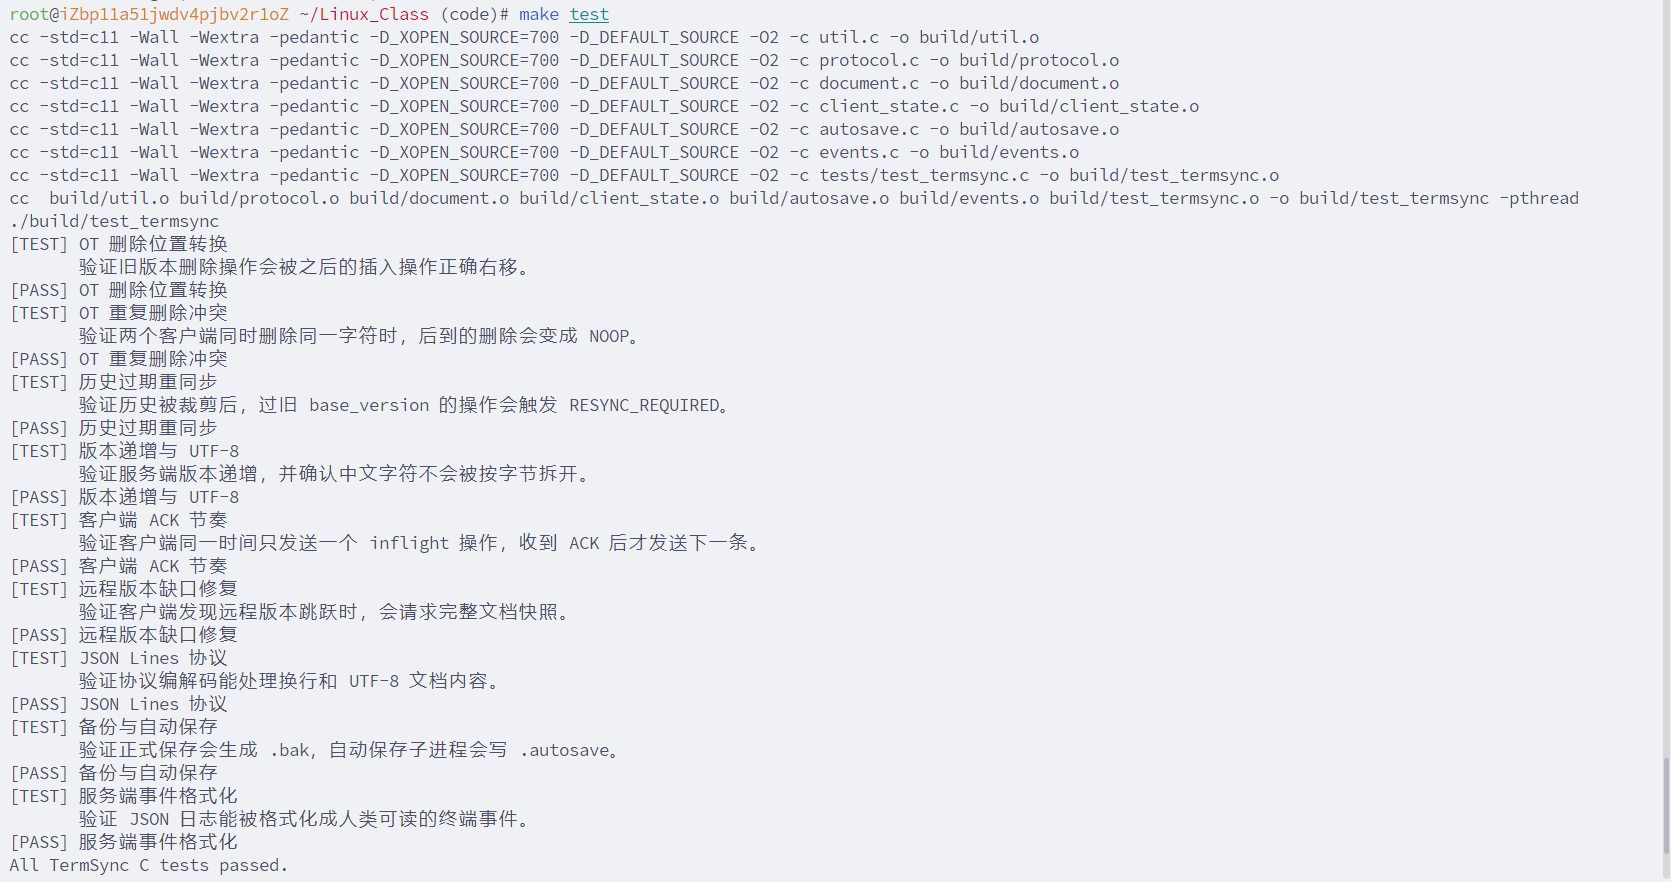
\includegraphics[width=0.8\textwidth]{pic/cowork/test1.png}
    \caption{测试结果}
\end{figure}


\subsubsection{本地验证}

本地验证用于在不依赖公网、域名解析和安全组规则的情况下，先确认协作编辑器本身的核心功能是否正常。验证时在同一台 Linux 服务器上进行：一个终端运行服务端，同时使用 \cmd{tmux} 打开两个客户端窗口进行对比观察。首先在服务端终端中监听本机地址并指定协作编辑文件：

\begin{minted}{bash}
python3 server.py --host 127.0.0.1 --port 8765 --file shared.py
\end{minted}

\begin{figure}[H]
    \centering
    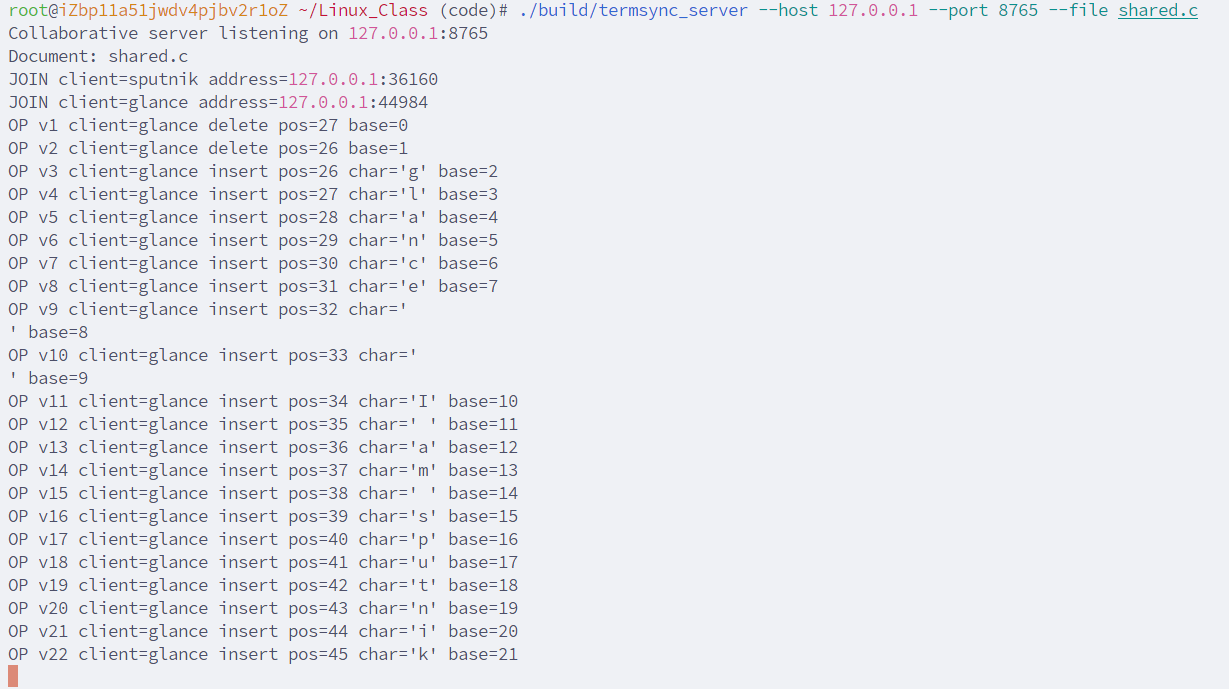
\includegraphics[width=0.8\textwidth]{pic/cowork/本地运行服务端.png}
    \caption{本地运行服务端界面}
\end{figure}

从服务端终端输出也可以看到，两个客户端加入时都会打印 \cmd{JOIN} 事件，并且地址字段中的 IP 均为 \cmd{127.0.0.1}。这说明 \cmd{sputnik} 和 \cmd{glance} 两个客户端虽然分别运行在不同的 \cmd{tmux} 窗口中，但网络连接都通过本机回环接口进入同一个服务端进程，符合本地手动验证的设计。

如果启动时出现 \cmd{Address already in use}，说明 \cmd{8765} 端口已经被已有进程占用，通常是前一次启动的服务端仍在运行。此时可以直接使用已有服务端继续启动客户端进行验证；如果需要重新启动服务端，则应先停止原服务端进程，或者临时换用其他端口并让两个客户端使用相同的新端口连接。

随后在 \cmd{tmux} 中打开两个客户端窗口或窗格，两个客户端都连接同一个本机服务端，但使用不同的 \cmd{client\_id}：

\begin{minted}{bash}
python3 client.py --host 127.0.0.1 --port 8765 --client-id sputnik
python3 client.py --host 127.0.0.1 --port 8765 --client-id glance
\end{minted}

\begin{figure}[H]
    \centering
    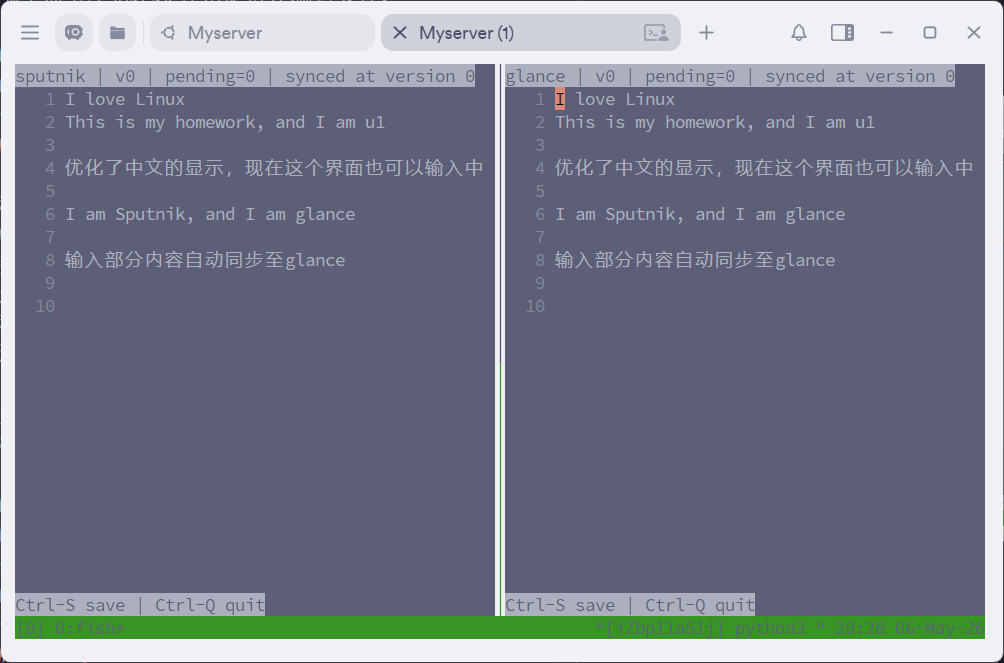
\includegraphics[width=0.95\textwidth]{pic/cowork/本地运行客户端界面.png}
    \caption{tmux 中两个本地客户端同步显示}
\end{figure}

图中左侧客户端使用 \cmd{sputnik}，右侧客户端使用 \cmd{glance}。两个客户端的状态栏都显示当前处于同步状态，文档内容也保持一致。实际验证时，在任意一个客户端输入英文、中文、换行或删除内容后，另一个客户端都会同步显示相同修改，说明本机环境下的消息发送、ACK 确认、服务端广播和客户端文档更新流程能够正常工作。

进一步验证异常情况时，可以在服务端终端中主动结束服务端进程。服务端关闭后，两个客户端不会继续显示为同步状态，而是在状态栏中显示 \cmd{error: connection closed}，提示与服务端的 TCP 连接已经断开；同时客户端中已经同步到的文档内容仍然保留在界面上，便于观察断线前的最终状态。

\begin{figure}[H]
    \centering
    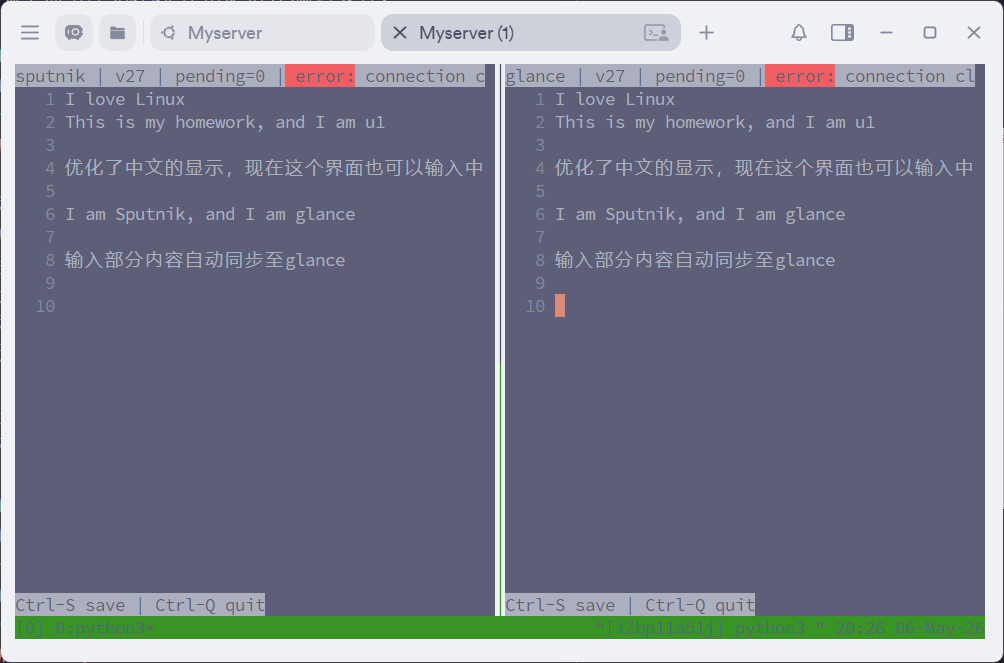
\includegraphics[width=0.95\textwidth]{pic/cowork/服务端关闭后客户端表现.png}
    \caption{服务端关闭后客户端显示连接断开}
\end{figure}

本地验证的价值在于把网络环境变量降到最低。如果本机回环地址下都无法完成同步，就说明问题大概率出现在客户端状态机、服务端文档模型或协议封装中；只有本地流程稳定后，再去验证公网域名、安全组和远程连接才有意义。实际调试时，我也按这个顺序推进，先在 \cmd{127.0.0.1} 上确认功能，再把服务端迁移到公网服务器运行。


\subsubsection{部署验证}

部署验证主要围绕真实公网运行流程展开。由于服务端运行在阿里云 ECS 服务器上，要让外部客户端能够访问该协作编辑服务，需要先在阿里云安全组中开放服务端使用的 \cmd{8765} 端口。只有安全组规则允许公网访问后，客户端才能通过 \cmd{glance02.xyz:8765} 连接到服务端。

\begin{figure}[H]
    \centering
    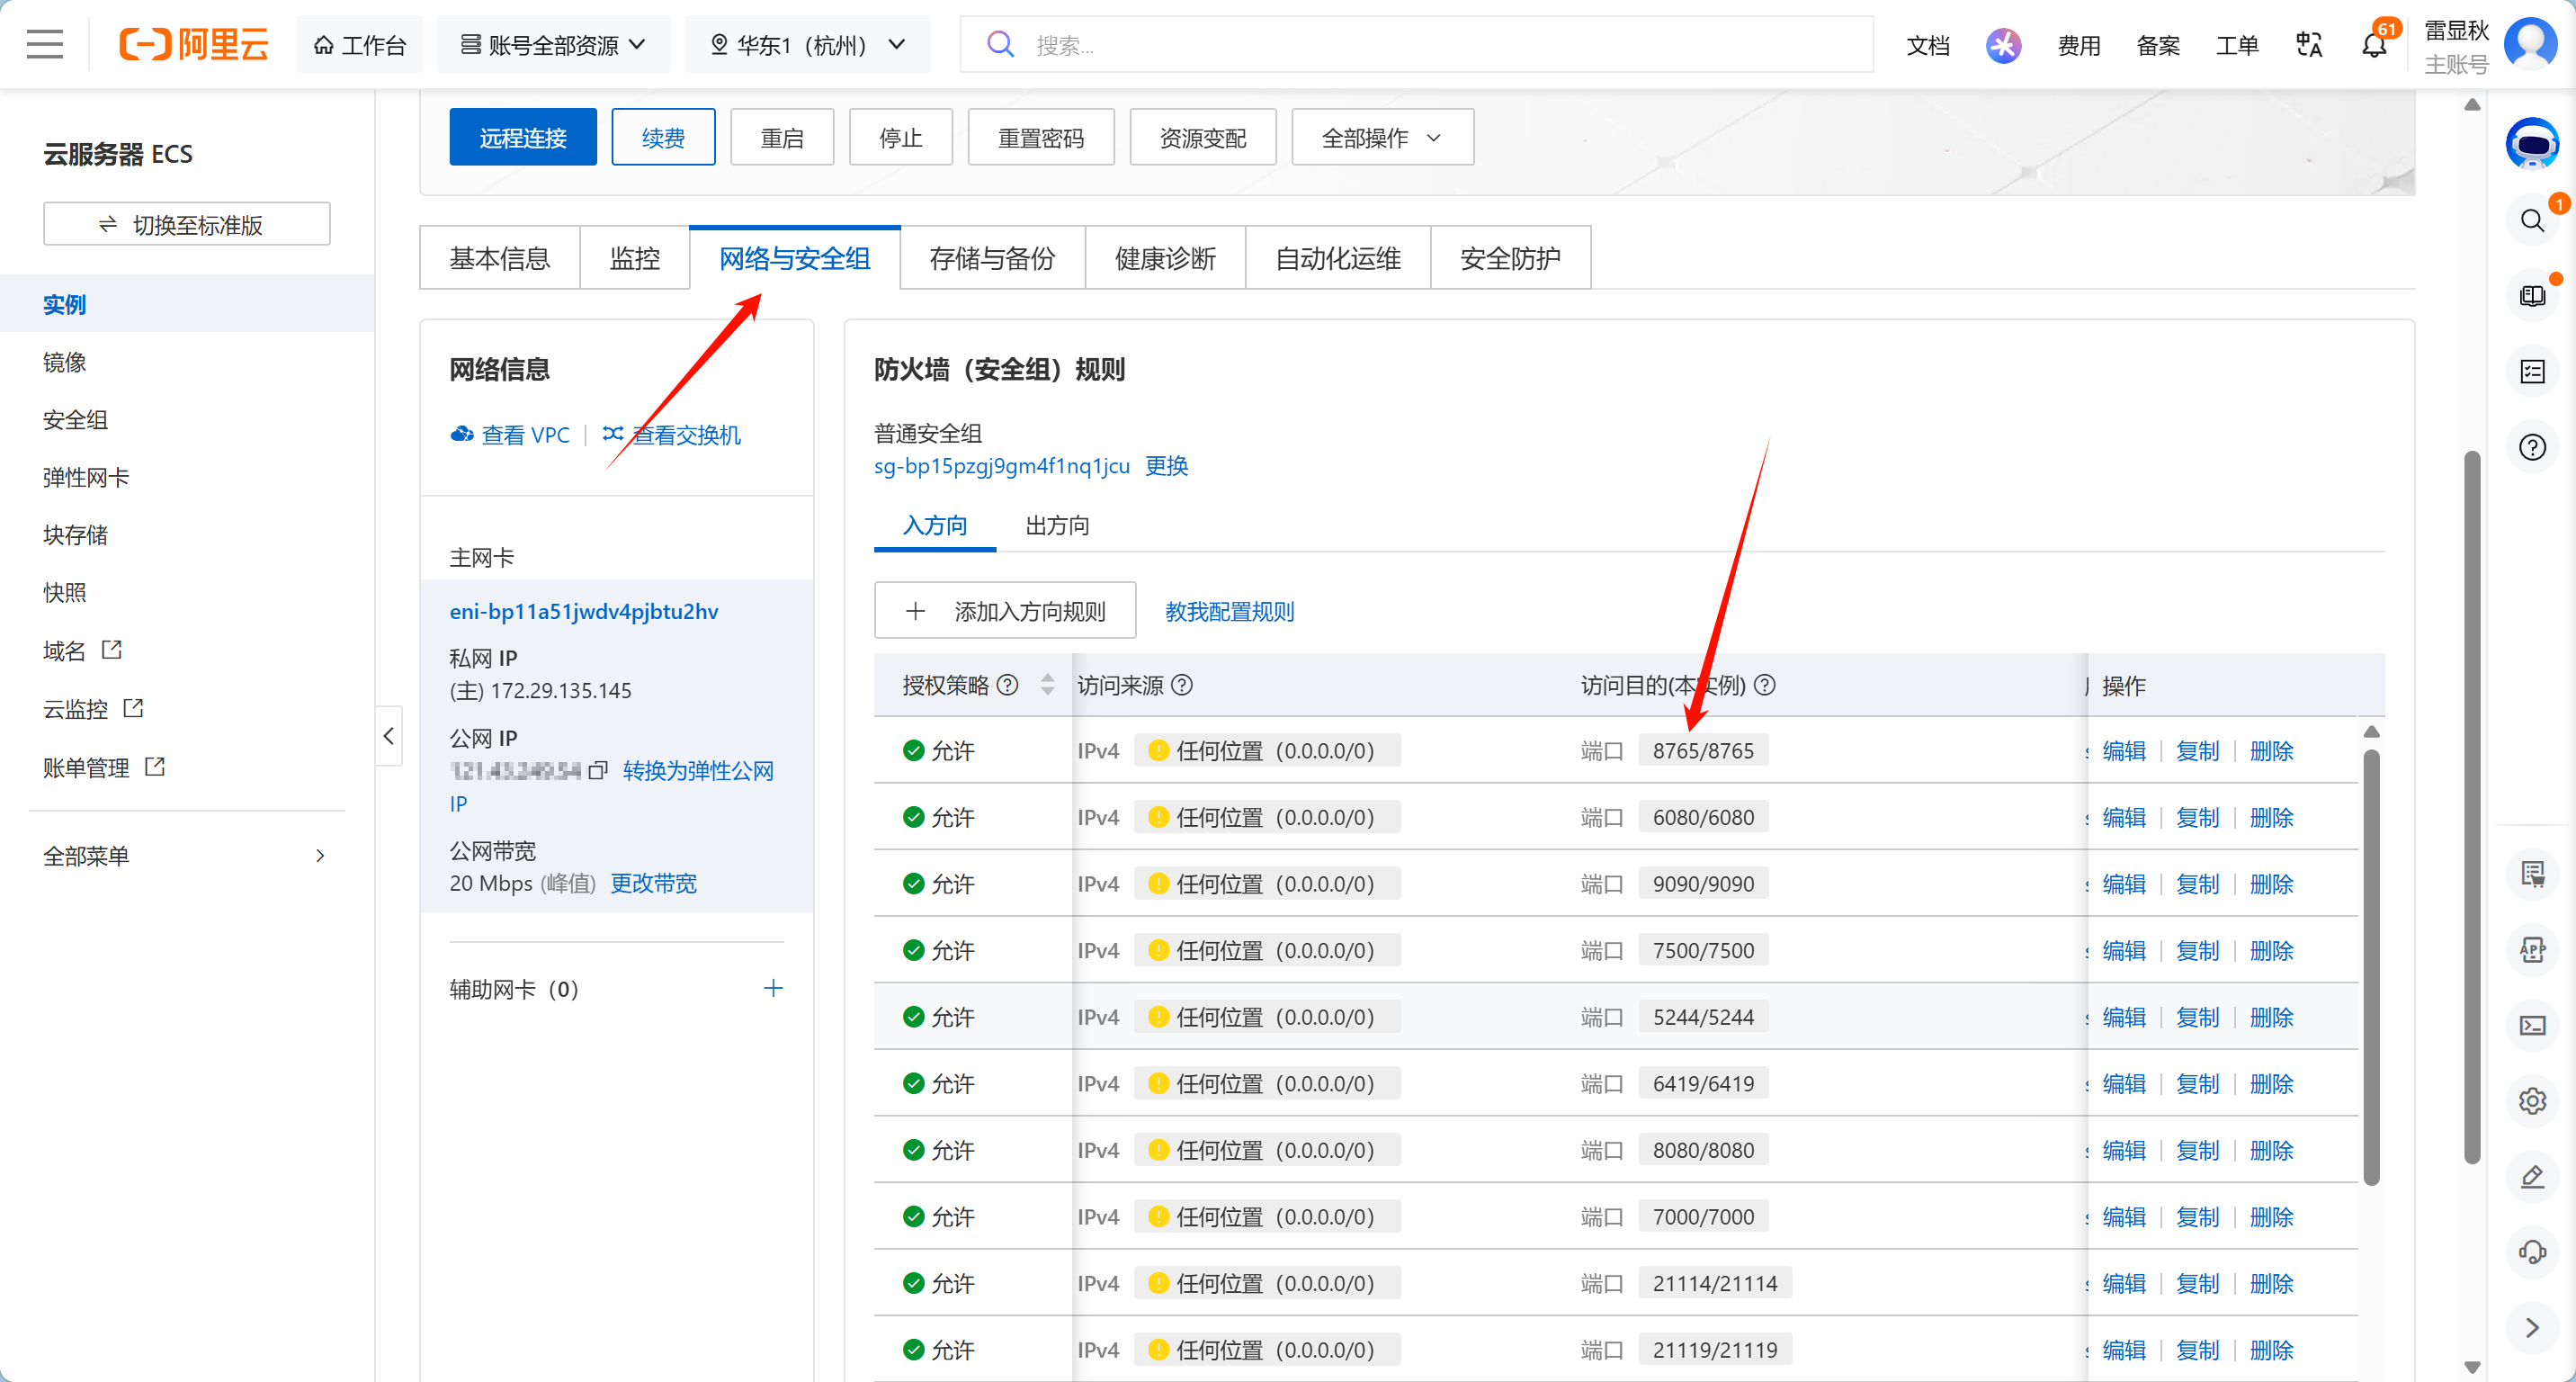
\includegraphics[width=0.8\textwidth]{pic/cowork/阿里云开放端口.png}
    \caption{阿里云开放8765端口}
\end{figure}

完成端口放行后，在 Linux 服务器上启动服务端，监听 \cmd{0.0.0.0:8765}，并指定协作编辑文件。由于服务器已经绑定域名 \cmd{glance02.xyz}，客户端可以直接通过该域名连接：

\begin{minted}{bash}
python3 client.py --host glance02.xyz --port 8765 --client-id u1
\end{minted}

随后在不同终端中启动两个客户端，分别使用不同 \cmd{client\_id}。当其中一个客户端输入字符或换行时，另一个客户端会收到 \cmd{REMOTE\_OP} 并同步显示更新。服务端终端会输出类似 \cmd{JOIN}、\cmd{OP v...}、\cmd{SAVE requested}、\cmd{LEAVE} 的事件日志，便于观察连接、编辑和保存流程。

下面是客户端 \cmd{sputnik} 连续输入换行和 \cmd{I am Sput} 时，服务端终端打印出的操作序列。可以看到每一次按键都会形成一条字符级 \cmd{insert} 操作，\cmd{v1} 到 \cmd{v10} 是服务端分配的全局递增版本号，\cmd{base} 则是客户端发送该操作时已确认的版本号。

\begin{minted}{text}
OP v1 client=sputnik insert pos=70 char='\n' base=0
OP v2 client=sputnik insert pos=71 char='I' base=1
OP v3 client=sputnik insert pos=72 char=' ' base=2
OP v4 client=sputnik insert pos=73 char='a' base=3
OP v5 client=sputnik insert pos=74 char='m' base=4
OP v6 client=sputnik insert pos=75 char=' ' base=5
OP v7 client=sputnik insert pos=76 char='S' base=6
OP v8 client=sputnik insert pos=77 char='p' base=7
OP v9 client=sputnik insert pos=78 char='u' base=8
OP v10 client=sputnik insert pos=79 char='t' base=9
\end{minted}

这段日志能够直接反映 ACK 驱动发送队列的效果：客户端收到上一条操作的 ACK 后才继续发送下一条，所以 \cmd{base} 会随着服务端版本逐步递增。另一方面，\cmd{pos} 也连续增加，说明服务端按字符位置把换行和后续英文字符顺序应用到了同一份权威文档中。

\begin{figure}[H]
    \centering
    \begin{minipage}{0.49\textwidth}
        \centering
        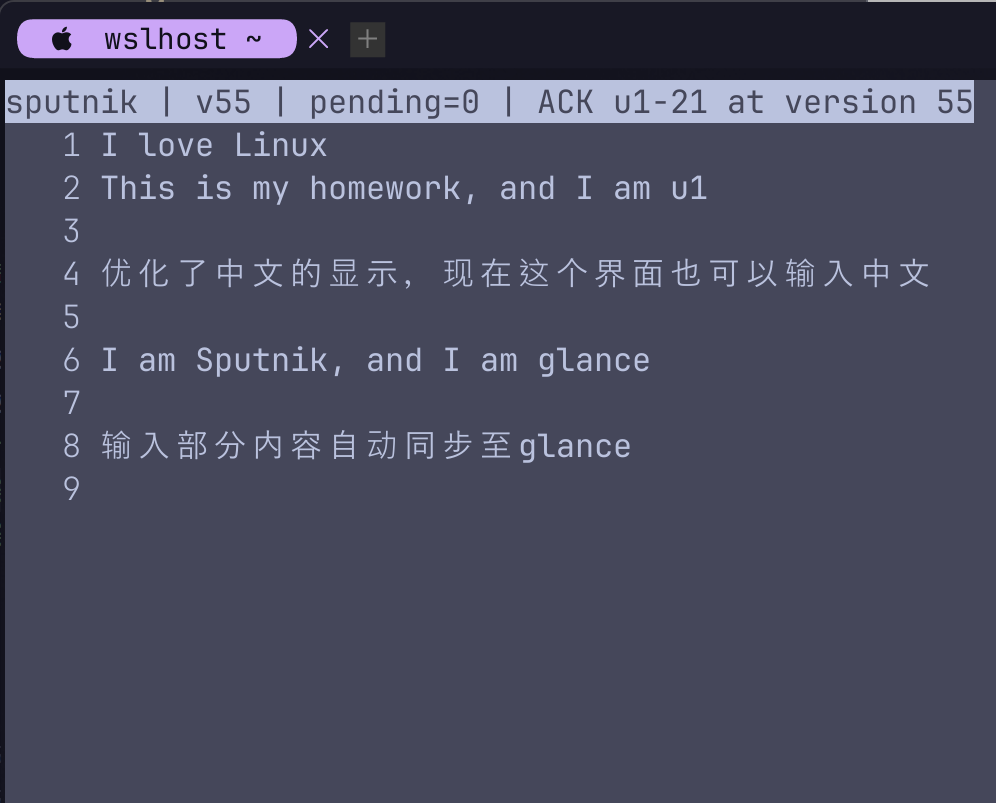
\includegraphics[width=\linewidth]{pic/cowork/client-sync-sputnik.png}
    \end{minipage}
    \hfill
    \begin{minipage}{0.49\textwidth}
        \centering
        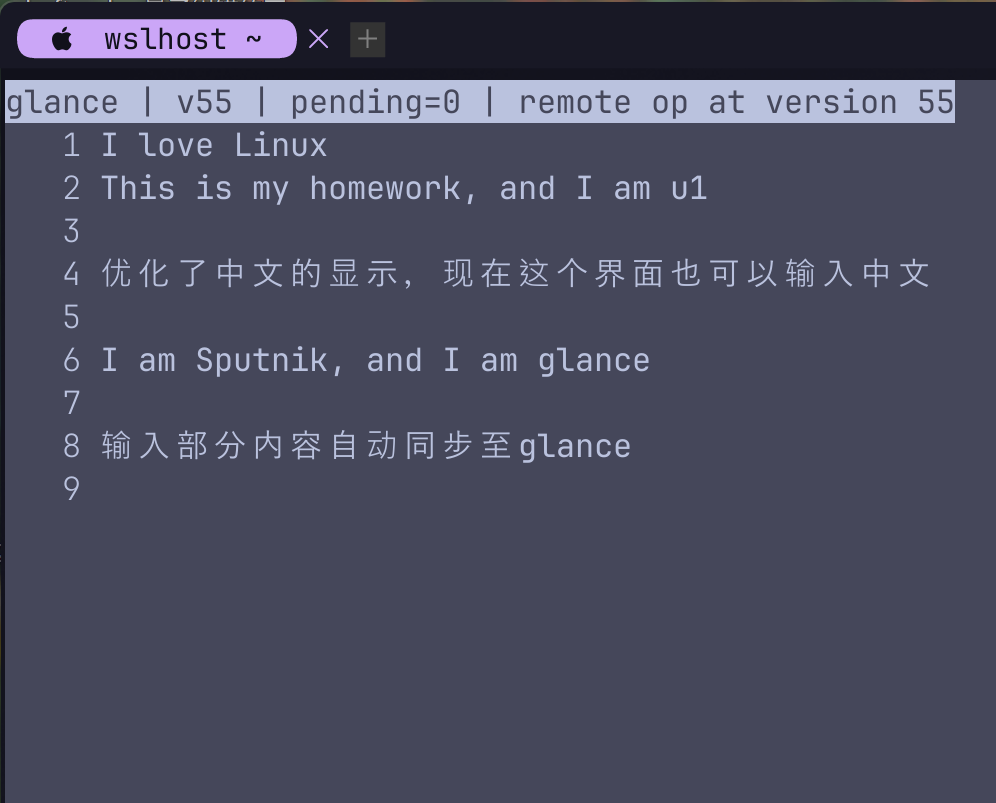
\includegraphics[width=\linewidth]{pic/cowork/client-sync-glance.png}
    \end{minipage}
    \caption{客户端 sputnik 输入内容后客户端 glance 自动同步显示}
\end{figure}

\begin{figure}[H]
    \centering
    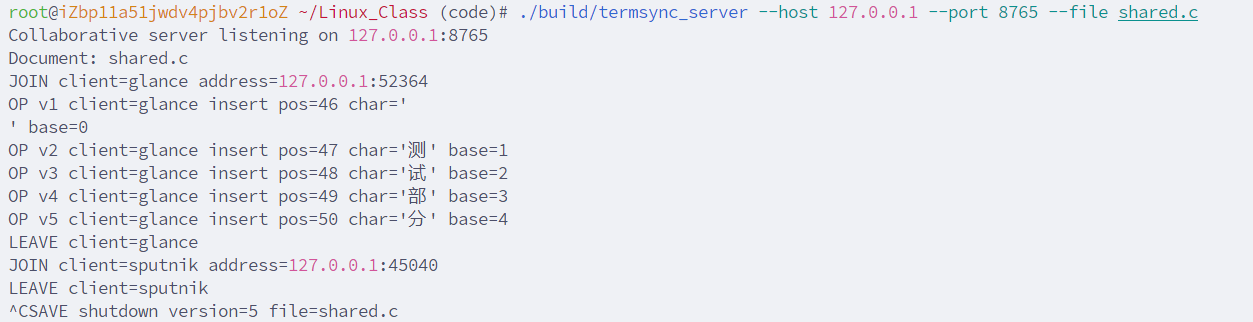
\includegraphics[width=0.95\textwidth]{pic/cowork/服务端界面日志.png}
    \caption{服务端终端输出 JOIN、OP、SAVE、LEAVE 等事件日志}
\end{figure}

为了验证 OT 行为，可以构造两个客户端基于不同版本编辑同一位置的场景。例如一个客户端连续在某个位置插入字符，另一个客户端基于旧版本删除该位置字符。根据服务端日志中的 \cmd{transform\_trace}，可以观察到操作位置在应用前被转换。最终两个客户端显示的文档内容保持一致。

\begin{figure}[H]
    \centering
    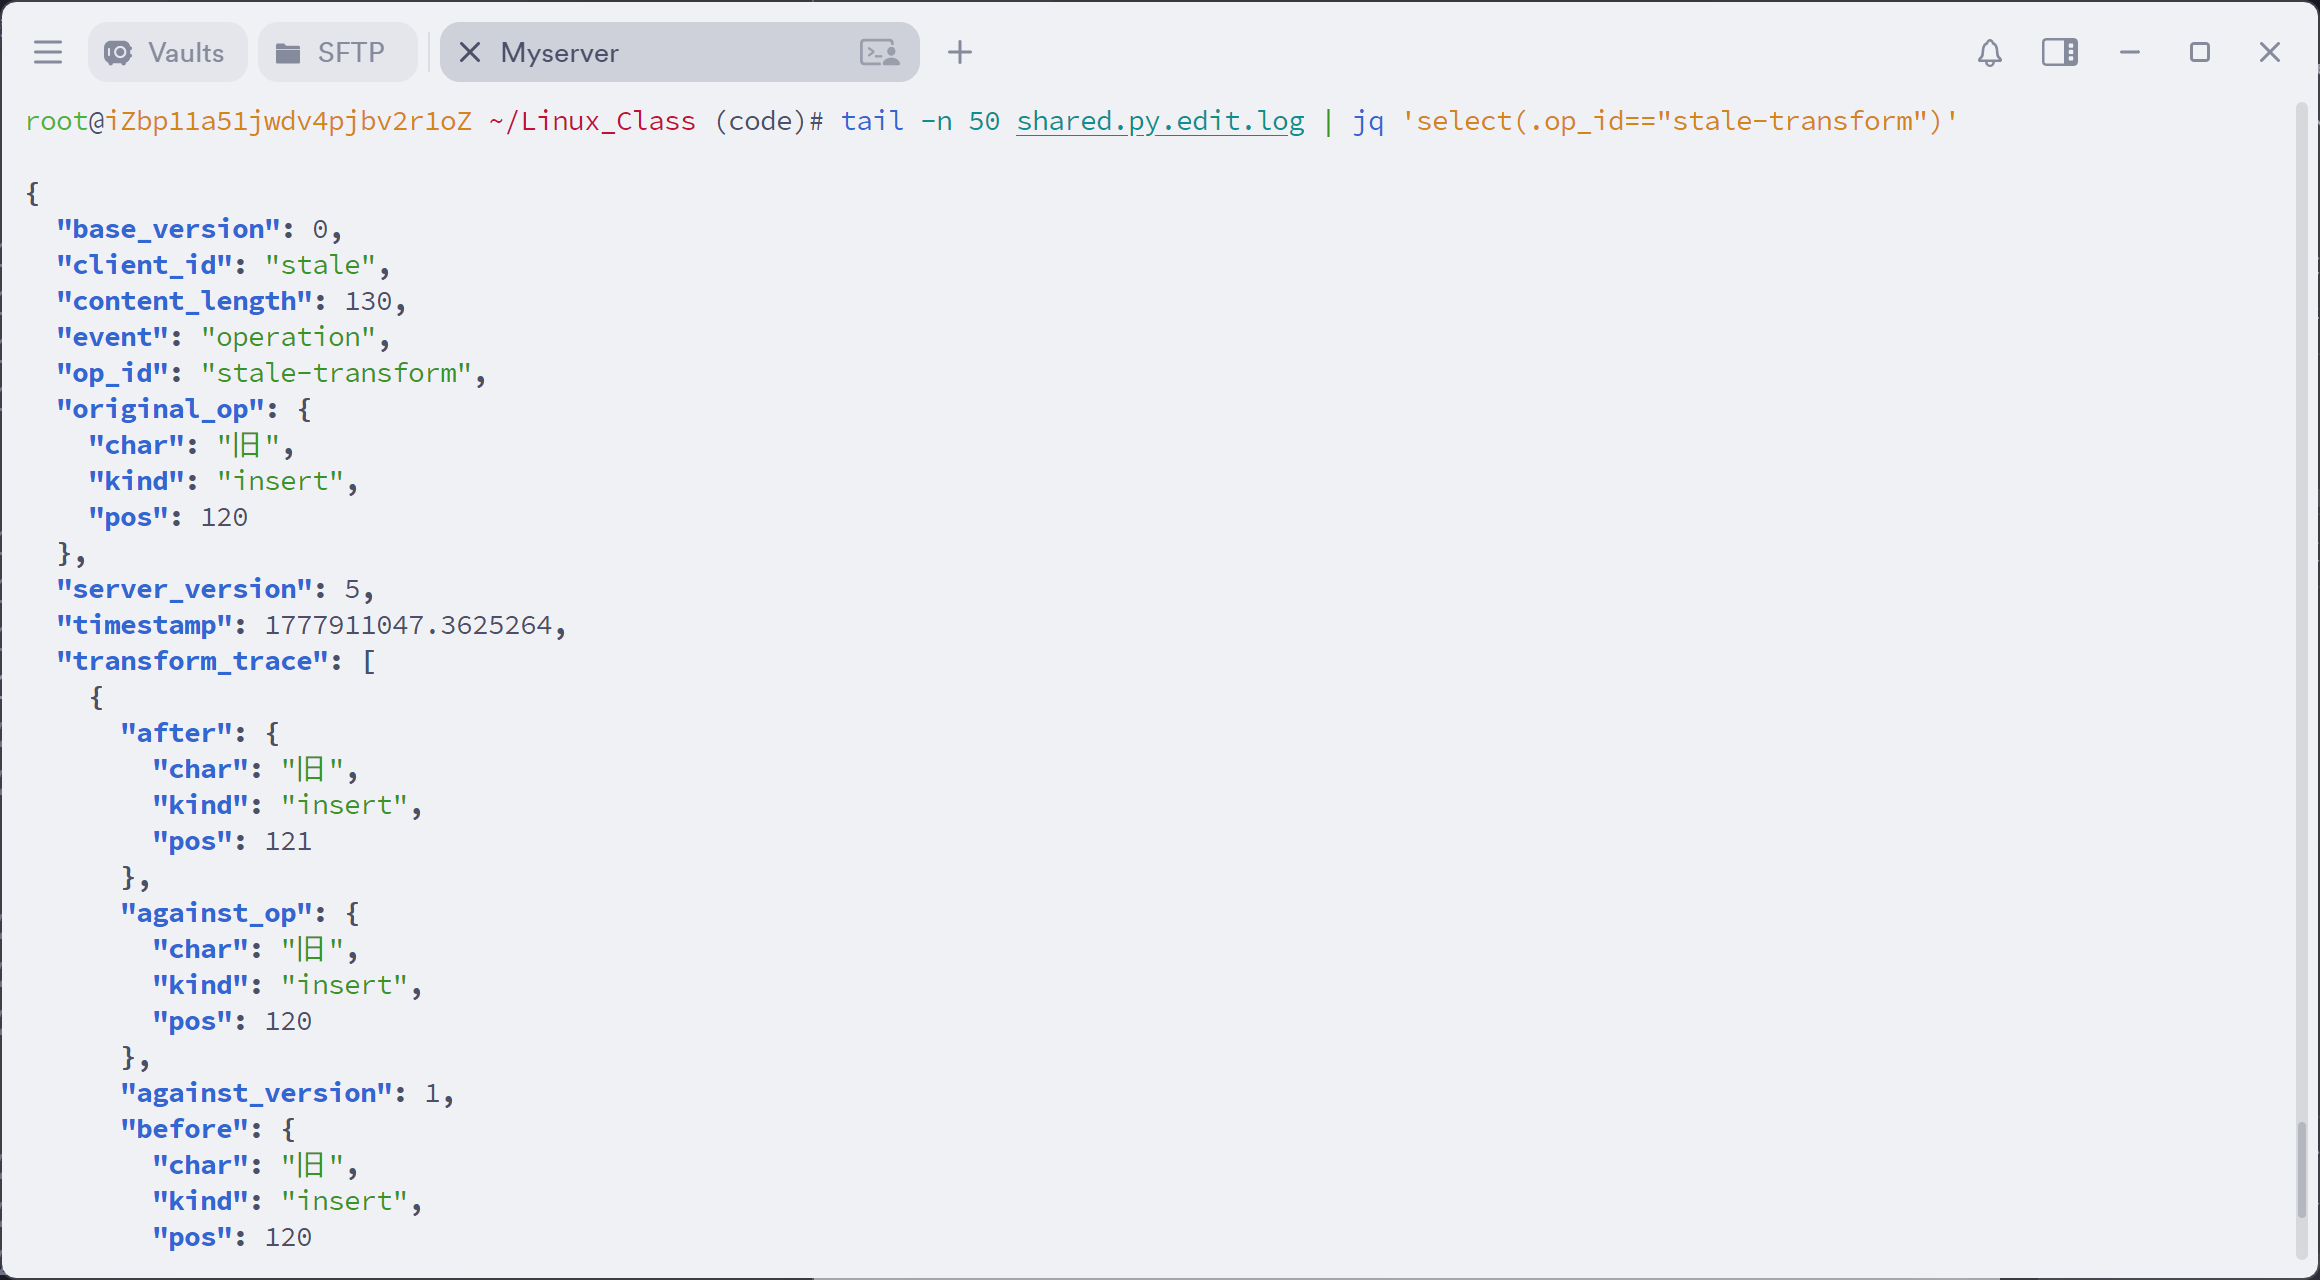
\includegraphics[width=0.95\textwidth]{pic/cowork/transform_trace日志.png}
    \caption{编辑日志中的 transform\_trace 位置变换记录}
\end{figure}

图中将原始 JSON 日志中的 \cmd{transform\_trace} 提取为位置变换过程。该操作的 \cmd{op\_id} 是 \cmd{stale-transform}，提交时基于旧版本 0，并在服务端版本 5 被确认。操作原本希望在位置 120 插入字符，服务端根据之后已经发生的历史插入操作依次调整位置，最终将其应用到位置 124。

\begin{table}[H]
    \centering
    \caption{\cmd{transform\_trace} 位置变换摘要}
    \small
    \begin{tabular}{c l c}
        \toprule
        \cmd{against\_version} & \cmd{against\_op} & \cmd{before\_pos} $\rightarrow$ \cmd{after\_pos} \\
        \midrule
        \cmd{1} & \cmd{insert(pos=120, char=旧)} & \cmd{120} $\rightarrow$ \cmd{121} \\
        \cmd{2} & \cmd{insert(pos=121, char=A)} & \cmd{121} $\rightarrow$ \cmd{122} \\
        \cmd{3} & \cmd{insert(pos=122, char=B)} & \cmd{122} $\rightarrow$ \cmd{123} \\
        \cmd{4} & \cmd{insert(pos=123, char=C)} & \cmd{123} $\rightarrow$ \cmd{124} \\
        \bottomrule
    \end{tabular}
\end{table}

该验证说明项目不仅可以在本机 \cmd{127.0.0.1} 上运行，也可以在真实网络环境中作为远程协作工具使用。相比本地验证，公网部署额外验证了域名解析、云服务器安全组、跨网络 TCP 连接和 WSL 客户端环境。特别是服务端监听 \cmd{0.0.0.0} 与客户端连接域名这两个细节，体现了服务器程序从“本机可用”走向“远程可访问”的差异。


部署过程中也能看到课程知识之间的联系。安全组端口放行属于网络访问控制，服务端监听和客户端连接属于 socket 编程，两个客户端同时编辑涉及线程并发，保存产物和日志属于文件系统操作，终端界面则依赖 Linux 命令行环境。这些内容在单独学习时可能是分散的知识点，但在 TermSync 中会组合成一个完整的运行链路。



\newpage
\subsection{问题与解决方案}

项目实现过程中遇到的问题并不是互相独立的。例如“连续输入容易乱序”与“旧版本操作位置失效”都和客户端本地版本落后有关；“慢客户端阻塞服务端”和“文件保存耗时”都和临界区范围有关；“中文字符显示宽度”虽然看起来只是界面问题，但如果光标位置换算错误，最终也会影响用户提交的编辑位置。因此本节按照问题来源整理解决方案，并说明这些方案在代码中的体现。


\subsubsection{并发操作顺序不确定}

问题：多个客户端线程可能同时提交编辑操作。如果服务端没有统一排序，不同线程对文档的修改顺序可能不稳定，客户端最终内容也可能不一致。

解决方案：将权威文档状态集中在服务端，并在 \cmd{CollaborativeDocument} 内部使用文档锁。每个操作进入锁保护的临界区后才分配 \cmd{server\_version}。因此全局顺序由服务端临界区顺序决定，而不是由客户端时间或网络延迟决定。

这个问题是整个项目中最基础的并发问题。服务端为每个客户端创建独立线程后，多个线程可能几乎同时调用文档处理函数。如果没有锁，两个线程可能读到相同的旧版本号，然后分别写入新文本，导致其中一次修改覆盖另一次修改。使用锁之后，文档对象内部的文本、版本号和历史记录成为一个整体状态，只能被一个线程按完整流程修改。

\subsubsection{旧版本操作位置失效}

问题：客户端提交操作时使用的是本地版本。如果该操作到达服务端时，其他客户端已经修改过文档，那么原始位置可能已经不再正确。

解决方案：服务端保存有限历史。处理旧版本操作时，从 \cmd{base\_version} 之后的历史操作开始逐条执行 OT 位置变换，将操作转换到当前版本后再应用。这样旧版本操作仍然能表达用户原本想编辑的位置。

这里不能简单拒绝所有旧版本操作，因为网络延迟本身就会让客户端操作在到达服务端时落后。如果每次落后都要求客户端完整重同步，协作编辑会频繁中断。有限历史和 OT 变换提供了折中方案：只要客户端的基准版本仍在服务端保留的历史范围内，就尽量通过位置变换保留用户意图；只有版本过旧、历史不足时，才触发重同步。

\subsubsection{连续输入容易丢失或乱序}

问题：用户在终端中快速输入多个字符时，如果客户端每次按键都立即发送，同时又没有处理未确认操作，容易造成本地版本混乱。

解决方案：客户端使用 \cmd{pending\_queue} 保存所有输入，并限制同一时刻最多一个 \cmd{inflight\_op}。只有收到当前操作的 ACK 后，才发送下一个操作。这样牺牲了一点发送并行度，但显著降低了客户端同步复杂度。

这个设计使客户端不需要预测远程操作对本地未确认操作的影响。用户快速输入时，按键不会丢失，而是依次进入待发送队列。客户端发送第一条操作后等待 ACK，ACK 到达后根据服务端返回的权威操作更新本地文本和版本，再发送下一条。这样每条新操作的 \cmd{base\_version} 都建立在已经确认的状态上，逻辑比全客户端 OT 简单很多。

\subsubsection{慢客户端可能阻塞服务端}

问题：如果服务端在文档锁内向所有客户端广播消息，而某个客户端网络很慢，socket 发送可能阻塞，从而导致其他客户端无法继续提交编辑操作。

解决方案：文档锁内只完成状态修改和消息构造，ACK 和广播都放在锁外执行。广播时也只短暂持有客户端列表锁来复制收件人列表，真正发送时不再持有该锁。

这个问题体现了临界区设计的重要性。锁保护的范围越大，程序越容易被慢操作拖住。socket 发送属于外部 I/O，耗时不可控，因此不适合放在文档锁内部。服务端先在锁内得到不可变的处理结果，再在锁外发送消息，就能同时保证文档状态一致和网络发送不阻塞后续文档处理。

\subsubsection{历史无限增长}

问题：如果服务端永久保存所有操作历史，长时间运行后内存占用会持续增加。

解决方案：历史记录使用有限长度队列保存最近的操作，最大条数由代码中的历史限制参数控制。同时维护 \cmd{history\_start\_version}，记录当前历史能够支持的最早基准版本。当客户端版本太旧，已经无法根据保留历史进行 OT 时，服务端返回 \cmd{RESYNC\_REQUIRED} 并发送完整文档。

历史裁剪使服务端可以长时间运行而不会随着编辑次数无限增加内存占用。代价是非常久未同步的客户端可能无法再用增量历史追上当前状态。对于这种客户端，完整文档重同步比继续尝试错误的 OT 更可靠。这个设计也说明系统需要在内存使用、实时性和恢复能力之间做取舍。

\subsubsection{文件保存可能覆盖旧内容}

问题：手动保存会覆盖正式文件，如果误操作或程序异常，可能丢失旧版本内容。

解决方案：保存前生成 \cmd{.bak} 备份文件，并使用临时文件替换的方式进行原子写入。自动保存则写入独立的 \cmd{.autosave} 文件，不直接覆盖正式文件。

保存策略没有把所有写入都混在同一个文件中，而是把正式保存、自动保存和备份分开。正式文档面向用户，自动保存面向异常恢复，备份面向误覆盖回退，日志面向调试追踪。多个文件共同构成一个更稳妥的保存体系，也让实验截图中可以直接观察到每种保存产物的存在。

\subsubsection{中文字符显示宽度}

问题：终端中中文字符通常占两个显示列，如果简单按照字符串长度移动光标，显示位置会错乱。

解决方案：客户端使用 Python 的 \cmd{unicodedata} 模块，通过 \cmd{east\_asian\_width} 判断宽字符，并提供显示列和字符列之间的转换函数。测试中也包含中文字符插入和显示宽度计算场景。

这个问题在图形界面程序中不一定明显，但在终端程序中非常常见。字符串索引表示的是字符数量，而终端光标移动使用的是显示列数；中文字符通常占两个显示列，如果直接把字符索引当作显示列，光标就会落到错误位置。本项目把文档内部索引和终端显示列分开处理，既能保持协议层的字符级操作简单，又能让终端显示符合用户直觉。

\newpage
\subsection{课程知识点对应关系}

TermSync 不是只调用某一个库完成单点功能，而是把网络、线程、进程、文件、终端和测试这些知识点组合到同一个可运行系统中。项目中的每个模块都可以对应到课程中的一个主题，运行时也能观察到这些主题之间的协作关系。

\begin{table}[H]
    \centering
    \caption{课程知识点与项目实现对应关系}
    \small
    \begin{tabular}{p{0.20\textwidth} p{0.28\textwidth} p{0.36\textwidth}}
        \toprule
        课程知识点 & 项目中的体现 & 实际作用 \\
        \midrule
        TCP 网络编程 & \cmd{server.py} 监听端口，\cmd{client.py} 主动连接 & 让多个终端客户端能够加入同一个协作文档 \\
        多线程 & 服务端为每个客户端创建处理线程 & 同时接收多个客户端消息，避免一个客户端独占服务端 \\
        线程同步 & \cmd{CollaborativeDocument} 内部使用锁 & 保证文本、版本号和历史记录的一致性 \\
        进程间通信 & 主服务端通过 \cmd{multiprocessing.Queue} 与保存进程通信 & 把磁盘写入从网络处理流程中拆出去 \\
        文件系统 & 正式文档、自动保存、备份、日志和临时文件 & 实现持久化、恢复和运行记录追踪 \\
        终端界面 & \cmd{curses} 绘制编辑区域和状态栏 & 在 Linux 命令行中提供交互式编辑体验 \\
        自动化测试 & \cmd{unittest} 覆盖文档、客户端状态和保存逻辑 & 用可重复测试验证同步算法和边界情况 \\
        \bottomrule
    \end{tabular}
\end{table}

\subsubsection{网络编程与长连接服务}

在基础命令和 Shell 脚本中，程序通常是短生命周期的：命令执行、输出结果、进程结束。而 TermSync 的服务端是一个长连接服务，它需要持续监听端口，反复接受客户端连接，并在连接存在期间不断接收消息。这使项目更接近真实 Linux 后台服务程序。

服务端启动时创建 socket，绑定地址和端口，然后进入监听状态。客户端通过 \cmd{connect} 与服务端建立 TCP 连接后，不是只发送一次请求就断开，而是在同一个连接上持续交换 JSON Lines 消息。这样的长连接模型适合协作编辑，因为每次按键都可能产生消息，如果每个字符都重新建立连接，延迟和开销都会变得很高。

网络编程中还必须考虑消息边界问题。TCP 提供的是字节流，不保证一次 \cmd{recv} 就对应一条完整业务消息。因此项目使用换行符作为消息边界，接收端维护缓冲区，只有读到完整一行后才进行 JSON 解码。这个设计虽然简单，但能直接解决粘包和拆包问题，也方便在服务端日志中观察原始消息流。

\begin{table}[H]
    \centering
    \caption{网络编程相关设计}
    \small
    \begin{tabular}{p{0.22\textwidth} p{0.30\textwidth} p{0.32\textwidth}}
        \toprule
        设计点 & 实现方式 & 课程意义 \\
        \midrule
        监听端口 & 服务端绑定 \cmd{host} 和 \cmd{port} 后调用监听接口 & 理解 TCP 服务端如何对外提供服务 \\
        客户端连接 & 客户端通过域名或 IP 连接服务端 & 理解客户端主动发起连接的过程 \\
        消息边界 & 使用 JSON Lines，每条消息以换行结束 & 理解 TCP 字节流和应用层协议的区别 \\
        发送互斥 & 协议封装中对同一 socket 发送加锁 & 避免多个线程同时写同一连接造成字节交叉 \\
        断线处理 & 连接关闭后客户端显示错误状态 & 让网络异常成为可观察状态，而不是静默失败 \\
        \bottomrule
    \end{tabular}
\end{table}

\subsubsection{线程同步与临界区控制}

多线程是服务端能够同时处理多个客户端的基础，但多线程也带来了共享状态竞争。TermSync 中最关键的共享状态是权威文档，包括文本内容、当前版本号和历史操作列表。如果两个线程同时修改这些状态，就可能出现版本号重复、文本内容覆盖或历史记录不完整等问题。

项目通过文档对象内部的锁来保护这些状态。每次处理客户端操作时，线程必须先进入临界区，然后检查客户端基准版本、执行位置变换、分配服务端版本、应用文本修改、写入历史记录。这个流程必须作为一个整体完成，不能只锁住其中一小步，否则仍然可能出现中间状态被其他线程观察到的问题。

另一方面，锁的范围也不能过大。网络发送、广播和磁盘保存都可能比较慢，如果把这些操作放在文档锁内部，慢客户端或慢磁盘就会阻塞所有编辑操作。因此项目把“状态修改”和“外部 I/O”分离：锁内只生成处理结果，锁外再发送 ACK、广播远程操作并投递保存事件。

\begin{table}[H]
    \centering
    \caption{临界区内外职责划分}
    \small
    \begin{tabular}{p{0.22\textwidth} p{0.32\textwidth} p{0.30\textwidth}}
        \toprule
        位置 & 执行内容 & 原因 \\
        \midrule
        文档锁内部 & 检查版本、执行 OT、修改文本、递增版本、写入历史 & 这些状态必须保持一致，不能被其他线程打断 \\
        文档锁外部 & 发送 ACK、广播远程操作、投递保存快照 & 这些操作涉及外部 I/O，耗时不可控 \\
        客户端表锁内部 & 复制当前在线客户端列表 & 防止遍历时客户端集合被修改 \\
        客户端表锁外部 & 真正向每个客户端发送消息 & 避免慢连接阻塞其他客户端加入或离开 \\
        保存进程内部 & 写入文件、生成备份、追加日志 & 磁盘操作独立于网络同步流程 \\
        \bottomrule
    \end{tabular}
\end{table}

\subsubsection{进程间通信与文件持久化}

服务端主进程负责网络同步，保存进程负责磁盘写入，这种拆分体现了进程间通信的使用。主进程处理完编辑操作后，不直接写文件，而是把快照和事件放入队列。保存进程从队列中取出事件，根据事件类型决定是更新自动保存内容、立即写入正式文件，还是追加日志。

这样设计的好处有两点。第一，主服务端不需要在每次按键后等待磁盘写入完成，可以继续处理其他客户端消息。第二，保存逻辑集中在独立模块中，更容易维护和测试。自动保存、手动保存、备份和日志都属于文件系统操作，把它们放在同一个进程函数中，代码边界更清晰。

文件持久化也不是简单地把字符串写入目标文件。项目中正式保存前会生成备份文件，自动保存写入独立的 \cmd{.autosave} 文件，日志使用 JSON Lines 追加记录事件，正式文件写入则尽量通过临时文件替换完成。这些设计共同降低了误覆盖、异常退出和写入中断带来的风险。

\begin{table}[H]
    \centering
    \caption{持久化事件与处理动作}
    \small
    \begin{tabular}{p{0.22\textwidth} p{0.30\textwidth} p{0.32\textwidth}}
        \toprule
        事件类型 & 来源 & 保存进程处理动作 \\
        \midrule
        快照更新 & 服务端成功处理编辑操作后投递 & 缓存最新文本和版本，等待自动保存时机 \\
        自动保存 & 保存进程定期触发 & 将最新快照写入 \cmd{.autosave} 文件 \\
        手动保存 & 客户端按下 \cmd{Ctrl-S} 后服务端投递 & 先生成 \cmd{.bak}，再写入正式文档 \\
        日志事件 & 加入、离开、操作、保存等服务端事件 & 追加一行 JSON 到 \cmd{.edit.log} \\
        停止事件 & 服务端关闭时投递 & 写入最终状态并结束保存进程 \\
        \bottomrule
    \end{tabular}
\end{table}

\subsubsection{终端交互与用户体验}

终端界面虽然没有图形界面复杂，但要做成可编辑工具仍然需要处理很多细节。客户端需要绘制状态栏、显示多行文本、根据光标位置滚动或定位，并把用户按键转换为编辑操作。普通字符、回车、Backspace、方向键、保存快捷键和退出快捷键都需要分别处理。

与普通命令行程序不同，\cmd{curses} 程序会接管终端屏幕，持续刷新显示内容。这要求客户端把“文档内部位置”和“屏幕显示位置”区分开。文档内部位置是字符串索引，协议和服务端都只关心这个索引；屏幕显示位置则要考虑换行、终端宽度和中文字符占用两列等问题。项目中专门实现字符宽度辅助函数，就是为了解决这个差异。

状态栏也是终端客户端的重要反馈。用户需要知道当前是否连接成功、是否正在等待 ACK、是否已经断线，以及应该如何保存或退出。虽然状态栏文字很短，但它让客户端不再是一个黑盒程序，用户可以根据状态判断下一步操作。

\subsubsection{测试驱动的课程项目验证}

课程项目不仅要能演示，还要能说明为什么它是可靠的。TermSync 的测试并不是覆盖所有界面细节，而是优先覆盖最核心的算法和状态变化。文档模型测试验证 OT 和版本一致性，客户端状态测试验证 ACK 队列和远程操作处理，保存测试验证备份行为，服务端输出测试保证演示日志稳定。

这种测试划分也体现了工程上的分层思想。越靠近核心模型的代码，越适合通过单元测试直接验证；越靠近终端界面和真实网络的部分，越适合通过手动验证和截图说明。把两种验证方式结合起来，既能保证核心逻辑可重复测试，也能说明程序在真实 Linux 环境中确实能够运行。

\begin{table}[H]
    \centering
    \caption{验证方式与适用范围}
    \small
    \begin{tabular}{p{0.22\textwidth} p{0.32\textwidth} p{0.30\textwidth}}
        \toprule
        验证方式 & 适合验证的内容 & 在报告中的体现 \\
        \midrule
        单元测试 & 文档变换、客户端队列、保存备份等确定性逻辑 & \cmd{unittest} 运行结果和测试覆盖表 \\
        本地手动验证 & 多客户端同步、断线显示、终端交互 & \cmd{127.0.0.1} 服务端和两个客户端截图 \\
        公网部署验证 & 域名连接、安全组端口、远程协作 & 阿里云端口开放和远程客户端连接截图 \\
        日志分析 & 操作顺序、版本递增、位置变换过程 & 服务端输出和 \cmd{transform\_trace} 表格 \\
        保存产物检查 & 自动保存、备份、正式文件和日志是否存在 & 保存目录截图和保存文件说明表 \\
        \bottomrule
    \end{tabular}
\end{table}

\newpage
\subsection{关键运行流程分解}

前面的设计说明从模块角度解释了系统结构，本节再从运行流程角度梳理 TermSync 的几个关键场景。这样可以更清楚地看到各模块在一次完整操作中如何协作，也能帮助阅读后面的代码展示部分。

\subsubsection{客户端加入流程}

客户端加入是整个协作流程的起点。客户端启动后先建立 TCP 连接，再发送 \cmd{JOIN} 消息。服务端收到后确认客户端编号，将连接保存到客户端表中，然后返回 \cmd{WELCOME} 和完整的 \cmd{DOC\_STATE}。只有拿到完整文档状态后，客户端才真正具备参与协作编辑的基础。

\begin{table}[H]
    \centering
    \caption{客户端加入流程}
    \small
    \begin{tabular}{p{0.14\textwidth} p{0.26\textwidth} p{0.42\textwidth}}
        \toprule
        步骤 & 执行方 & 说明 \\
        \midrule
        1 & 客户端 & 解析命令行参数，得到服务端地址、端口和客户端编号 \\
        2 & 客户端 & 创建 socket，并连接服务端监听地址 \\
        3 & 客户端 & 发送 \cmd{JOIN} 消息，请求加入协作文档 \\
        4 & 服务端线程 & 接收连接并读取加入消息，确认或调整客户端编号 \\
        5 & 服务端线程 & 将连接对象加入在线客户端表 \\
        6 & 服务端线程 & 返回 \cmd{WELCOME} 和当前完整 \cmd{DOC\_STATE} \\
        7 & 客户端 & 初始化本地文档、版本号和同步状态，进入编辑界面 \\
        \bottomrule
    \end{tabular}
\end{table}

这个流程中最重要的是完整文档状态的发送。新客户端不需要从历史第一条操作开始回放，而是直接接收服务端当前权威文本和版本号。这样即使服务端已经运行了一段时间，新加入的客户端也能快速追上当前状态。

\subsubsection{编辑操作确认流程}

用户按下普通字符、回车或 Backspace 后，客户端并不直接把本地文档当作最终结果，而是把按键转换成操作对象并放入发送队列。发送队列根据 ACK 节奏向服务端提交操作。服务端在文档锁内处理操作，生成权威结果后再通知各个客户端。

\begin{table}[H]
    \centering
    \caption{编辑操作确认流程}
    \small
    \begin{tabular}{p{0.14\textwidth} p{0.26\textwidth} p{0.42\textwidth}}
        \toprule
        步骤 & 执行方 & 说明 \\
        \midrule
        1 & 客户端界面 & 读取用户按键，将其转换为 \cmd{insert} 或 \cmd{delete} 操作 \\
        2 & 客户端状态机 & 把操作加入 \cmd{pending\_queue}，等待发送机会 \\
        3 & 客户端状态机 & 如果当前没有 \cmd{inflight\_op}，取队首操作发送 \cmd{OP} 消息 \\
        4 & 服务端文档对象 & 在锁内检查版本、执行 OT、规范化位置并应用操作 \\
        5 & 服务端文档对象 & 分配新的 \cmd{server\_version}，写入历史记录 \\
        6 & 服务端线程 & 向提交者发送 \cmd{ACK}，向其他客户端发送 \cmd{REMOTE\_OP} \\
        7 & 客户端状态机 & 收到 ACK 后应用权威操作，清空 \cmd{inflight\_op} 并继续发送队列 \\
        8 & 其他客户端 & 收到远程操作后检查版本连续性，并应用到本地文档 \\
        \bottomrule
    \end{tabular}
\end{table}

这个流程把客户端和服务端的职责分得比较清楚。客户端负责把用户意图变成操作并按顺序发送，服务端负责确认操作在全局历史中的位置。只要客户端最终应用的是服务端确认后的权威操作，即使多个客户端输入时间非常接近，也能收敛到同一个文档内容。

\subsubsection{保存与关闭流程}

保存流程分为自动保存、手动保存和关闭时保存。自动保存用于降低异常退出风险，手动保存用于响应用户明确操作，关闭时保存用于服务端退出前尽量保留最终内容。三者都通过保存进程完成，而不是直接在客户端处理线程中写文件。

\begin{table}[H]
    \centering
    \caption{保存与关闭流程}
    \small
    \begin{tabular}{p{0.18\textwidth} p{0.28\textwidth} p{0.36\textwidth}}
        \toprule
        场景 & 触发方式 & 处理过程 \\
        \midrule
        自动保存 & 服务端处理成功操作后投递最新快照 & 保存进程缓存最新内容，并按固定间隔写入 \cmd{.autosave} \\
        手动保存 & 用户在客户端按下 \cmd{Ctrl-S} & 服务端投递保存事件，保存进程生成备份并写入正式文件 \\
        日志追加 & 客户端加入、离开、编辑、保存等事件发生 & 保存进程追加 JSON Lines 日志，记录事件时间和版本 \\
        服务端关闭 & 用户中断服务端或程序退出 & 服务端向保存进程投递最终保存和停止事件 \\
        客户端断开 & 客户端退出或网络连接关闭 & 服务端移除连接，并向日志记录离开事件 \\
        \bottomrule
    \end{tabular}
\end{table}

从这个流程可以看出，保存进程并不是简单附属功能，而是项目可靠性的一部分。如果没有自动保存，服务端异常退出可能导致大量未保存编辑丢失；如果没有备份文件，手动保存可能覆盖用户原有内容；如果没有编辑日志，就很难解释某次演示中操作顺序和位置变换为什么会那样发生。

\subsubsection{重同步流程}

重同步用于处理客户端状态和服务端状态差距过大的情况。正常情况下，客户端通过 ACK 和远程操作逐步跟上服务端；但如果客户端漏收消息、网络断开后重连，或者提交操作时基准版本已经早于服务端保留的历史起点，服务端就无法可靠地执行增量 OT。此时继续尝试变换反而可能产生错误结果。

\begin{table}[H]
    \centering
    \caption{重同步触发与恢复}
    \small
    \begin{tabular}{p{0.22\textwidth} p{0.30\textwidth} p{0.32\textwidth}}
        \toprule
        触发原因 & 服务端或客户端判断 & 恢复方式 \\
        \midrule
        客户端提交版本太旧 & \cmd{base\_version} 早于 \cmd{history\_start\_version} & 服务端返回 \cmd{RESYNC\_REQUIRED} 和完整文档 \\
        客户端发现版本跳跃 & 收到的远程版本不是本地版本加一 & 客户端发送 \cmd{REQUEST\_DOC} 请求完整状态 \\
        新客户端加入 & 本地没有任何文档状态 & 服务端直接发送当前 \cmd{DOC\_STATE} \\
        未确认操作失效 & 重同步后旧的 \cmd{inflight\_op} 不再可靠 & 客户端清空待确认状态，以服务端文档为准 \\
        \bottomrule
    \end{tabular}
\end{table}

重同步体现了系统对异常状态的保守处理原则：当增量同步已经不可靠时，优先回到服务端权威快照，而不是继续叠加可能错误的操作。对于课程项目而言，这个机制也让历史裁剪变得可行，因为服务端不需要永久保存所有操作，只需要在历史不足时提供完整文档恢复路径。

\newpage
\subsection{项目不足与改进方向}

虽然 TermSync 已经能够完成多人连接、实时同步、保存、自动保存、日志记录和测试验证，但它仍然是一个课程项目规模的协作编辑器，和成熟协作工具相比还存在一些不足。首先，当前编辑粒度是字符级操作，便于说明 OT 原理，但快速输入大量文本时会产生较多网络消息；后续可以考虑把连续输入合并为批量操作。其次，系统暂时没有加入用户认证和权限控制，只适合可信网络或课堂演示场景，如果要公开部署，需要补充连接鉴权、访问控制和异常客户端隔离。再次，客户端的终端界面功能较基础，还可以继续增加状态栏、只读提示、断线重连和冲突恢复提示，使使用体验更加完整。

从实现角度看，后续还可以继续扩展测试范围。例如增加更复杂的并发插入、插入与删除交错、历史裁剪后客户端重连等集成测试；在服务端加入更细粒度的运行日志和错误统计；在保存模块中加入异常注入测试，验证磁盘写入失败时备份文件和自动保存文件是否仍然可靠。这些改进能够进一步提升项目的稳定性，也能让课程报告中的系统设计更加接近真实 Linux 服务程序。

\newpage
\subsection{代码展示}

本文所对应的项目代码托管于 GitHub 仓库 \url{https://github.com/glance02/Linux_Class.git}。其中，程序实现位于 \cmd{code} 分支，论文正文的 LaTeX 源码位于 \cmd{master} 分支。项目完整实现包含服务端、客户端、协议封装、持久化、日志和测试等多个模块，代码量较大；受篇幅限制，本节仍以关键代码片段为主。下文代码展示中涉及的文件路径，均以服务器克隆 \cmd{code} 分支后得到的代码仓库根目录为基准。

\subsubsection{项目结构}

TermSync 的项目实现代码位于 GitHub 仓库的 \cmd{code} 分支。下面的结构以克隆并切换到 \cmd{code} 分支后的仓库根目录为基准，按照客户端、服务端、文档模型、协议封装、持久化进程和测试代码进行划分：

\begin{minted}[fontsize=\small,breaklines]{text}
Linux_Class/
|-- autosave.py              # 自动保存、手动保存、备份和日志写入进程
|-- client.py                # curses 终端客户端与键盘交互逻辑
|-- client_state.py          # 客户端 ACK 队列、版本同步和远程操作处理
|-- document.py              # 权威文档模型、操作定义、OT 变换和历史管理
|-- protocol.py              # JSON Lines 协议编码、解码和 socket 收发封装
|-- server.py                # TCP 服务端、客户端线程、广播和保存触发
|-- README.md                # 项目运行方式与功能说明
|-- plan.md                  # 项目设计与实现计划记录
|-- main.tex                 # 项目代码分支中的说明文档
`-- tests/
    |-- test_autosave.py     # 自动保存和备份逻辑测试
    |-- test_client_state.py # 客户端状态机与宽字符处理测试
    |-- test_document.py     # 文档一致性、OT 和重同步测试
    `-- test_server.py       # 服务端事件输出和关闭逻辑测试
\end{minted}

其中，\cmd{server.py}、\cmd{document.py}、\cmd{autosave.py} 构成服务端核心；\cmd{client.py} 和 \cmd{client\_state.py} 构成终端客户端；\cmd{protocol.py} 则被客户端和服务端共同使用，用于保证两端消息格式一致。\cmd{tests} 目录中的单元测试覆盖了同步算法、客户端状态、保存备份和服务端输出等关键行为。

\subsubsection{协议与基础数据结构}

\textbf{协议封装：}协作编辑首先需要稳定的消息边界和统一的数据表示。项目使用 JSON Lines 作为 TCP 字节流上的应用层协议：发送时把 Python 字典编码为 UTF-8 JSON，并在末尾追加换行符；接收时先在缓冲区中寻找换行符，再解码出完整消息。协议封装还为发送操作加锁，避免同一连接被多个线程同时写入时出现字节交叉。

\inputminted[firstline=1,lastline=77,firstnumber=1]{python}{code/cowork/protocol.py}

\textbf{操作模型：}编辑操作、历史记录和处理结果集中定义在 \cmd{document.py} 中。\cmd{Operation} 表示字符级 \cmd{insert}、\cmd{delete} 和 \cmd{noop}，并在从网络消息解析时进行类型检查；\cmd{HistoryEntry} 保存已经进入服务端全局顺序的历史操作；\cmd{ProcessResult} 则把文档处理结果拆成 ACK、广播消息、日志和快照，方便服务端在锁外执行网络发送和磁盘保存。

\inputminted[firstline=1,lastline=112,firstnumber=1]{python}{code/cowork/document.py}

\subsubsection{服务端权威文档与 OT}

\textbf{文本应用与位置变换：}文本修改函数负责把规范化后的操作真正作用到字符串上，而 OT 变换函数负责根据历史操作修正位置。当一个客户端操作基于旧版本提交时，服务端会把它依次与之后已经发生的历史操作比较，修正位置偏移；如果两个删除操作指向同一个字符，后到达的删除会变为 \cmd{noop}，从而避免误删后续字符。

\inputminted[firstline=115,lastline=160,firstnumber=115]{python}{code/cowork/document.py}

\textbf{权威文档处理流程：}\cmd{CollaborativeDocument} 是服务端的权威文档对象。它使用 \cmd{RLock} 保护文本、版本号和有限历史记录，所有编辑操作只有进入该临界区后才会分配递增的服务端版本号。\cmd{process\_operation} 展示了完整处理流程：解析操作、检查版本、执行 OT、规范化位置、应用文本、写入历史，并生成后续需要发送或保存的结果。

\inputminted[firstline=162,lastline=329,firstnumber=162]{python}{code/cowork/document.py}

\textbf{重同步辅助逻辑：}当客户端版本太旧时，服务端需要返回完整文档快照；当操作位置越界时，服务端也要在应用前进行规范化。下面的内部辅助函数负责生成快照、筛选历史、规范化操作，并维护当前历史仍能支持的最早 \cmd{base\_version}。

\inputminted[firstline=331,lastline=369,firstnumber=331]{python}{code/cowork/document.py}

\subsubsection{服务端连接、广播与保存触发}

\textbf{事件输出与连接对象：}服务端一方面要维护面向用户的运行日志，另一方面要为每个客户端连接保存必要信息。下面的代码展示了终端日志格式化函数和 \cmd{ClientConnection}。这些格式化函数不改变协议内容，只把结构化事件转换成便于演示观察的 \cmd{JOIN}、\cmd{OP}、\cmd{SAVE} 等文本。

\inputminted[firstline=1,lastline=75,firstnumber=1]{python}{code/cowork/server.py}

\textbf{初始化、监听与关闭：}\cmd{CollaborativeServer} 在启动时读取协作文档、创建权威文档对象、准备客户端连接表，并启动独立的自动保存进程。监听循环使用 TCP socket 接受客户端连接，每个连接交给一个线程处理；关闭时则向保存进程发送最终保存和停止事件，保证文档内容能够落盘。

\inputminted[firstline=77,lastline=184,firstnumber=77]{python}{code/cowork/server.py}

\textbf{客户端消息处理：}客户端线程先完成加入握手，并向新客户端返回欢迎消息和完整文档状态。后续消息由分发函数按类型处理：编辑操作进入文档模型，保存请求投递保存队列，文档请求则直接返回最新快照。操作处理完成后，服务端在文档锁外发送 ACK 和广播，从而避免慢客户端阻塞文档临界区。

\inputminted[firstline=193,lastline=282,firstnumber=193]{python}{code/cowork/server.py}

\textbf{广播、日志与命令行入口：}服务端将成功操作的快照交给自动保存进程，把结构化事件写入日志，并在复制客户端列表后执行广播。最后的入口函数通过 \cmd{argparse} 提供监听地址、端口、协作文档路径、历史长度和自动保存间隔等参数，并注册信号处理函数，使 \cmd{Ctrl-C} 停止服务端时也能走统一清理流程。

\inputminted[firstline=283,lastline=385,firstnumber=283]{python}{code/cowork/server.py}

\subsubsection{客户端状态机与终端界面}

\textbf{客户端同步状态：}客户端同步状态的关键是 \cmd{pending\_queue} 和 \cmd{inflight\_op}。用户连续输入产生的操作先进入队列；同一时刻客户端最多发送一个未确认操作，收到服务端 ACK 后再发送下一个。客户端应用的始终是服务端返回的权威操作，因此不需要在本地实现复杂 OT。

\inputminted[firstline=1,lastline=145,firstnumber=1]{python}{code/cowork/client_state.py}

\textbf{终端宽字符与光标换算：}终端客户端需要在一维文档索引、行列坐标和实际屏幕显示列之间转换。由于中文等宽字符在终端中通常占两个显示列，代码中使用 \cmd{unicodedata} 判断字符宽度，并提供显示列与字符列之间的转换函数，保证中英文混排时光标移动仍能对齐。

\inputminted[firstline=1,lastline=114,firstnumber=1]{python}{code/cowork/client.py}

\textbf{curses 客户端主体：}\cmd{TerminalClient} 把网络接收和 curses 界面分开：后台线程只负责从 socket 读取消息并放入队列，界面线程负责消费消息、渲染状态栏和正文，并把用户按键转换为 \cmd{Operation}。普通字符、回车和 Backspace 会变成协作编辑操作，\cmd{Ctrl-S} 和 \cmd{Ctrl-Q} 分别用于保存和退出。

\inputminted[firstline=117,lastline=289,firstnumber=117]{python}{code/cowork/client.py}

\textbf{客户端入口：}客户端入口读取服务端地址、端口和客户端编号，并设置系统 \cmd{locale}，使 curses 能够在终端中正确处理中文输入和宽字符显示。

\inputminted[firstline=291,lastline=307,firstnumber=291]{python}{code/cowork/client.py}

\subsubsection{自动保存、备份与日志}

\textbf{保存进程：}自动保存和日志写入放在独立进程中完成，主服务端只通过进程间队列投递快照、保存请求和日志事件。\cmd{atomic\_write\_text} 使用临时文件替换目标文件，降低写入中断造成半截文件的风险；手动保存会先复制旧文件生成 \cmd{.bak}，再写入正式文件；自动保存则写入独立的 \cmd{.autosave} 文件。

\inputminted[firstline=1,lastline=120,firstnumber=1]{python}{code/cowork/autosave.py}

\subsubsection{单元测试}

\textbf{文档一致性测试：}这一组测试直接验证服务端权威文档模型，也是 OT 正确性的核心证据。测试包括旧版本删除位置经过多次插入后右移、重复删除同一字符变为 \cmd{noop}、历史过期触发重同步、服务端版本严格递增，以及中文字符能够作为单字符插入。

\inputminted[firstline=1,lastline=120,firstnumber=1]{python}{code/cowork/tests/test_document.py}

\textbf{客户端状态测试：}这一组测试说明客户端为什么不会在连续输入时丢操作。它验证了 ACK 驱动发送队列、远程版本缺口请求完整文档、服务端重新分配客户端编号、中文字符可插入、宽字符显示宽度计算，以及 Backspace 会排队生成删除操作。

\inputminted[firstline=1,lastline=114,firstnumber=1]{python}{code/cowork/tests/test_client_state.py}

\textbf{服务端输出测试：}这一组测试不启动真实 socket，而是检查服务端可观察输出是否稳定。测试覆盖插入、删除、保存、客户端加入和离开事件的格式化结果，同时验证非服务端主进程调用 \cmd{shutdown} 时不会错误地关闭父进程资源。

\inputminted[firstline=1,lastline=75,firstnumber=1]{python}{code/cowork/tests/test_server.py}

\textbf{自动保存备份测试：}这一组测试聚焦文件保存行为。通过 mock 隔离真实文件系统后，测试验证手动保存覆盖正式文件前会先复制原文件生成 \cmd{.bak} 备份，然后再调用原子写入函数写入新内容。

\inputminted[firstline=1,lastline=28,firstnumber=1]{python}{code/cowork/tests/test_autosave.py}

\newpage

% Add your chapter files here when needed.
\section{Linux 平台下的基本命令}

作业中要求使用 Linux 平台进行操作，我使用一台阿里云 ECS 服务器完成实验。服务器配置为 2 核 2 GB，操作系统为 Ubuntu 24.04。本次实验通过 SSH 连接到服务器，并在真实 Linux 环境中完成命令演示。我使用 Termius 作为 SSH 客户端，便于在 Windows 电脑上远程连接服务器。

本节按照文件和目录、文件内容处理、系统信息、权限管理以及管道组合五类来整理命令。这样比单纯罗列命令更容易看出不同命令的使用场景，也能体现 Linux 命令之间可以组合使用的特点。

\begin{table}[H]
    \centering
    \caption{基础命令分类与实验目标}
    \small
    \begin{tabular}{p{0.20\textwidth} p{0.34\textwidth} p{0.30\textwidth}}
        \toprule
        命令类别 & 代表命令 & 实验目标 \\
        \midrule
        文件和目录 & \cmd{pwd}、\cmd{ls}、\cmd{mkdir}、\cmd{cp}、\cmd{mv}、\cmd{rm} & 熟悉路径、目录层次和文件生命周期操作 \\
        内容查看与处理 & \cmd{cat}、\cmd{head}、\cmd{tail}、\cmd{wc}、\cmd{sort}、\cmd{uniq}、\cmd{grep} & 学会从文本文件中查看、筛选、排序和统计内容 \\
        系统信息 & \cmd{uname}、\cmd{whoami}、\cmd{date}、\cmd{df}、\cmd{free}、\cmd{ps} & 观察当前 Linux 系统、资源和进程状态 \\
        权限管理 & \cmd{ls -l}、\cmd{chmod}、\cmd{stat} & 理解读、写、执行权限以及脚本可执行条件 \\
        管道组合 & \cmd{|}、\cmd{grep}、\cmd{sort}、\cmd{uniq}、\cmd{wc} & 把多个小工具组合成完整的数据处理流程 \\
        \bottomrule
    \end{tabular}
\end{table}

\subsection{文件和目录操作}

\begin{enumerate}
\item 查看当前所在目录：\cmd{pwd}
\item 查看当前目录下的文件：\cmd{ls}
\item 以详细形式查看文件：\cmd{ls -l}
\item 查看隐藏文件：\cmd{ls -a}

\begin{figure}[H]
    \centering
    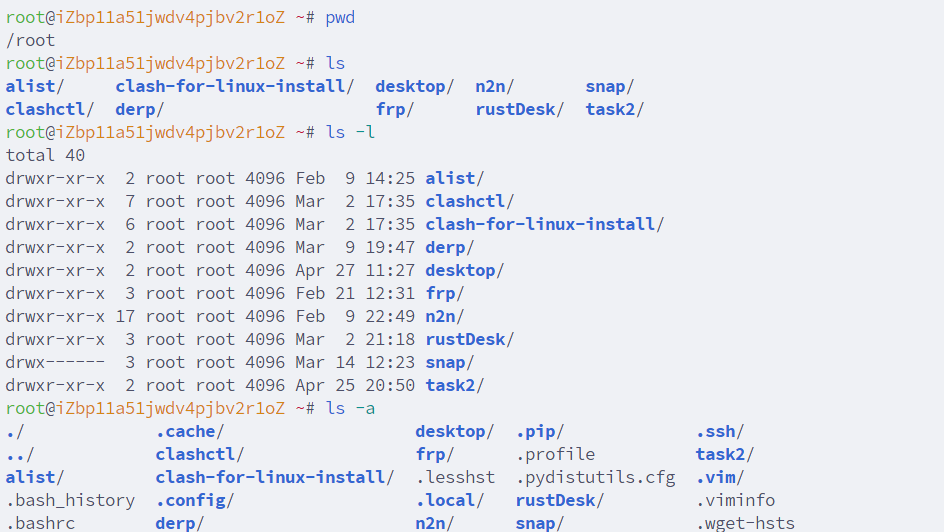
\includegraphics[width=0.8\textwidth]{pic/task1/image.png}
    \caption{命令1.1-1.4}
\end{figure}

\item 创建一个目录：\cmd{mkdir linux\_test}
\item 进入目录：\cmd{cd linux\_test}
\item 创建空文件：\cmd{touch file1.txt}
\item 向文件写入内容：\cmd{echo "hello linux" > file1.txt}
\item 查看文件内容：\cmd{cat file1.txt}
\item 复制文件：\cmd{cp file1.txt file2.txt}

\begin{figure}[H]
    \centering
    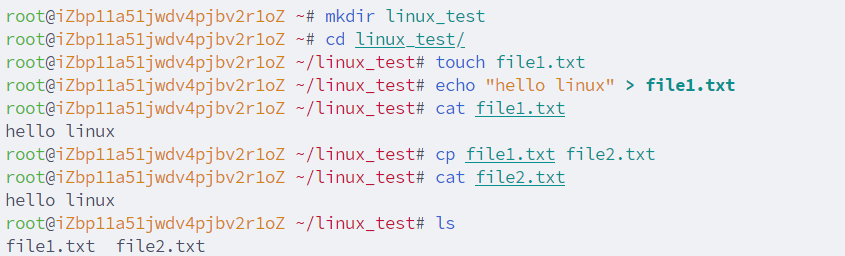
\includegraphics[width=0.8\textwidth]{pic/task1/image copy.png}
    \caption{命令1.5-1.10}
\end{figure}

\item 重命名文件：\cmd{mv file1.txt newfile.txt}
\item 删除文件：\cmd{rm newfile.txt}
\item 返回上一级目录：\cmd{cd ..}
\item 删除目录：\cmd{rm -r linux\_test}

\begin{figure}[H]
    \centering
    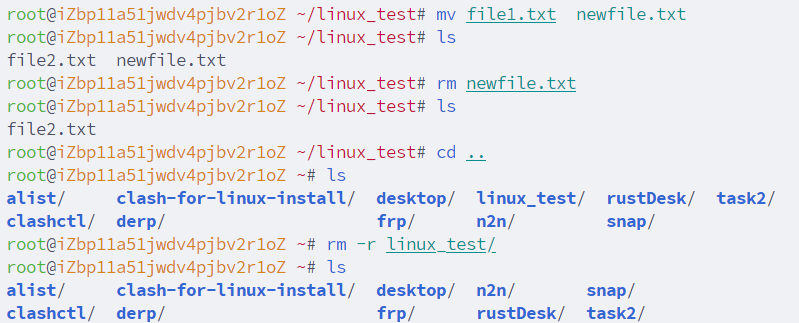
\includegraphics[width=0.8\textwidth]{pic/task1/image copy 2.png}
    \caption{命令1.11-1.14}
\end{figure}

\end{enumerate}

这一组命令展示了 Linux 中文件从创建、写入、复制、重命名到删除的完整过程。需要注意的是，\cmd{rm} 和 \cmd{rm -r} 都属于不可逆的删除操作，真实使用时应先通过 \cmd{pwd} 和 \cmd{ls} 确认当前目录和目标文件，避免在错误目录下删除内容。目录操作中，\cmd{cd ..} 表示返回父目录，\cmd{./} 表示当前目录，理解这些相对路径写法后，后续执行脚本和引用文件会更清晰。

\begin{table}[H]
    \centering
    \caption{文件目录命令使用要点}
    \small
    \begin{tabular}{p{0.18\textwidth} p{0.28\textwidth} p{0.36\textwidth}}
        \toprule
        命令 & 常用场景 & 注意点 \\
        \midrule
        \cmd{pwd} & 查看当前工作目录 & 执行删除、复制前先确认位置，避免误操作 \\
        \cmd{ls -la} & 同时查看详细信息和隐藏文件 & 以点号开头的文件默认不会被普通 \cmd{ls} 显示 \\
        \cmd{mkdir} & 创建项目目录或实验目录 & 如果父目录不存在，需要先创建父目录或使用合适路径 \\
        \cmd{cp} & 复制文件作为备份 & 复制目录时通常需要加 \cmd{-r} 参数 \\
        \cmd{mv} & 移动文件或重命名文件 & 同名目标可能被覆盖，执行前要确认目标路径 \\
        \cmd{rm -r} & 删除目录及其中内容 & 风险较高，实验中只对临时目录使用 \\
        \bottomrule
    \end{tabular}
\end{table}

\subsection{文件内容查看与处理命令}

我先使用如下命令创建测试目录和测试文件，然后再对文件内容处理命令进行演示。

\begin{minted}{bash}
mkdir linux_homework
cd linux_homework
echo -e "apple\nbanana\napple\norange\nbanana\nlinux\ncommand\npipe" > words.txt    
\end{minted}

\begin{enumerate}
\item 查看完整内容：\cmd{cat words.txt}

\begin{figure}[H]
    \centering
    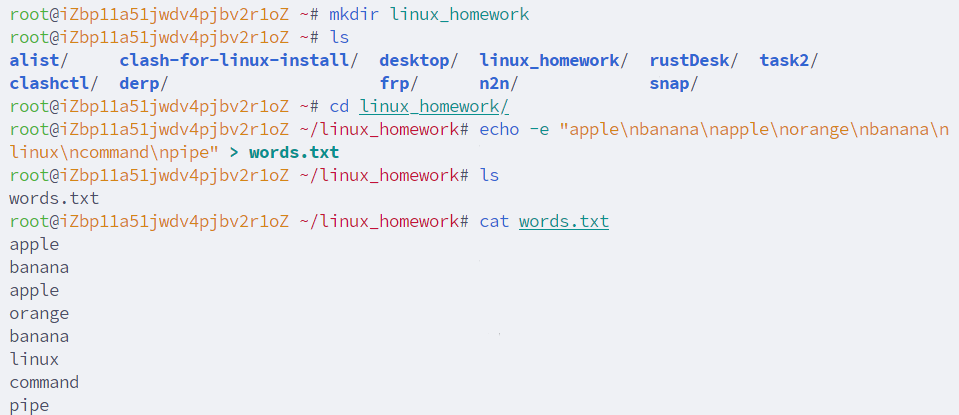
\includegraphics[width=0.8\textwidth]{pic/task1/image copy 3.png}
    \caption{命令2.1}
\end{figure}

\item 查看文件前3行：\cmd{head -n 3 words.txt}
\item 查看文件后3行：\cmd{tail -n 3 words.txt}
\item 统计文件行数、单词数、字符数：\cmd{wc words.txt}
\item 统计文件行数：\cmd{wc -l words.txt}
\begin{figure}[H]
    \centering
    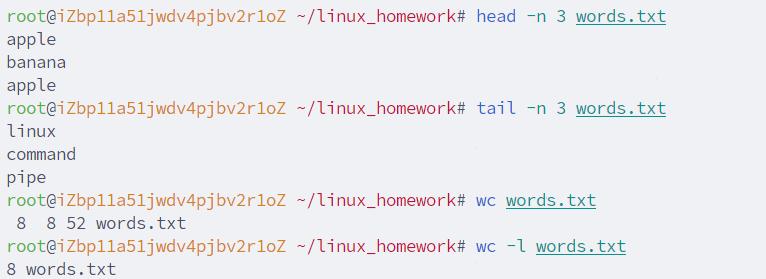
\includegraphics[width=0.8\textwidth]{pic/task1/image copy 4.png}
    \caption{命令2.2-2.5}
\end{figure}

\item 对文件内容排序：\cmd{sort words.txt}
\item 去除相邻重复行：\cmd{uniq words.txt}
\item 查找包含 apple 的行：\cmd{grep "apple" words.txt}
\item 查找包含 banana 的行，并显示行号：\cmd{grep -n "banana" words.txt}

\begin{figure}[H]
    \centering
    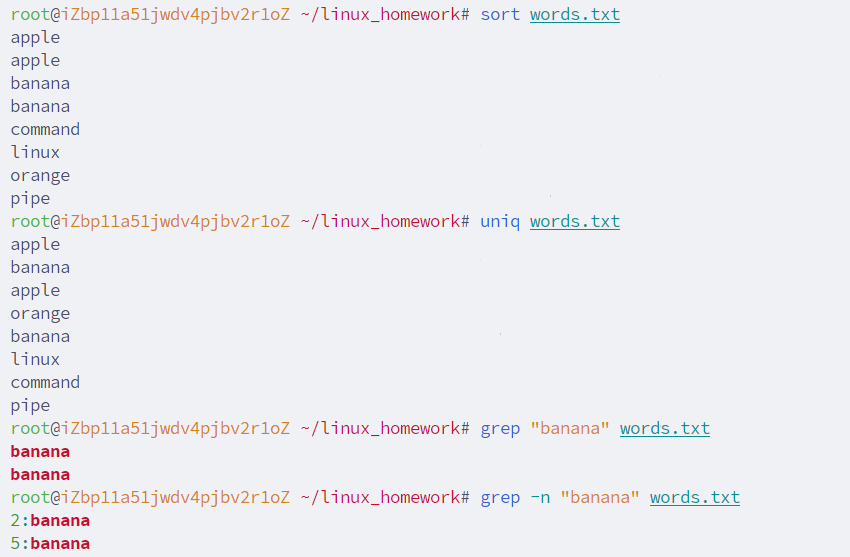
\includegraphics[width=0.8\textwidth]{pic/task1/image copy 5.png}
    \caption{命令2.6-2.9}
\end{figure}

\cmd{uniq} 只能去除相邻的重复行，如果重复内容之间隔着其他行，直接执行 \cmd{uniq words.txt} 并不能完成全局去重。因此在后面的管道命令中，我又使用 \cmd{sort words.txt | uniq}，先把相同内容排到相邻位置，再进行去重统计。

\end{enumerate}

文件内容处理命令体现了 Linux 把文本作为基础数据格式的特点。很多配置、日志、题库和脚本都可以被看作普通文本文件，因此掌握查看、筛选、统计和排序命令后，就可以在不打开图形化编辑器的情况下快速定位信息。例如查看日志时常用 \cmd{tail -n 50} 看末尾几十行，统计题库行数时可以使用 \cmd{wc -l}，从大量输出中查找关键词时可以使用 \cmd{grep}。

\begin{table}[H]
    \centering
    \caption{文本处理命令对比}
    \small
    \begin{tabular}{p{0.18\textwidth} p{0.30\textwidth} p{0.34\textwidth}}
        \toprule
        命令 & 适合解决的问题 & 本次实验中的体现 \\
        \midrule
        \cmd{cat} & 快速查看小文件完整内容 & 查看 \cmd{words.txt} 中的全部测试单词 \\
        \cmd{head} / \cmd{tail} & 只查看文件开头或结尾 & 验证文件前 3 行和后 3 行内容 \\
        \cmd{wc} & 统计行数、单词数和字符数 & 判断测试文件规模和行数 \\
        \cmd{sort} & 按字典序排列文本行 & 为去重和词频统计做准备 \\
        \cmd{uniq} & 合并相邻重复行 & 与 \cmd{sort} 配合完成全局去重 \\
        \cmd{grep} & 按关键词筛选文本行 & 查找包含指定单词的行，并显示行号 \\
        \bottomrule
    \end{tabular}
\end{table}

\subsection{系统信息查看命令}

\begin{enumerate}
\item 查看系统内核和系统信息：\cmd{uname -a}
\item 查看当前用户名：\cmd{whoami}
\item 查看当前日期时间：\cmd{date}
\item 显示日历：\cmd{cal}

\begin{figure}[H]
    \centering
    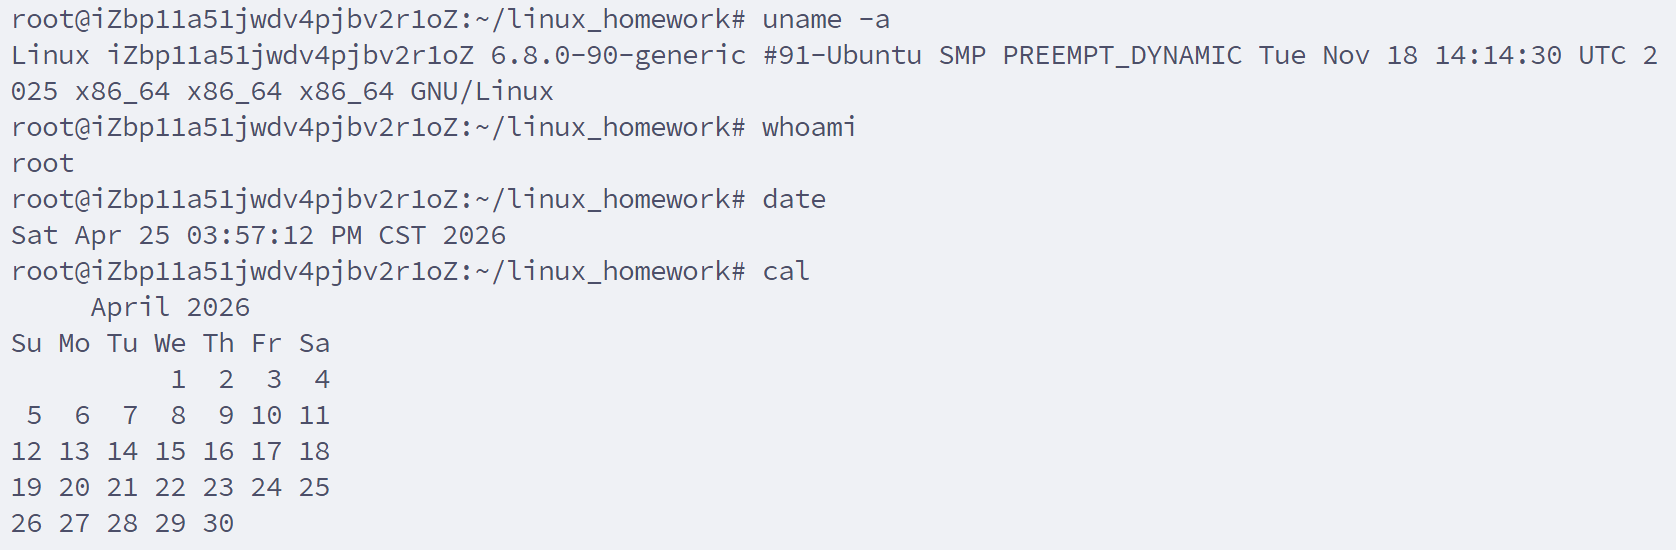
\includegraphics[width=0.8\textwidth]{pic/task1/image copy 6.png}
    \caption{命令3.1-3.4}
\end{figure}

如果系统默认没有安装 \cmd{cal} 命令，需要先安装 \cmd{ncal} 包。我使用 \cmd{sudo apt install ncal} 安装之后，就可以正常显示日历。

\item 查看磁盘空间：\cmd{df -h}
\item 查看内存使用情况：\cmd{free -h}

\begin{figure}[H]
    \centering
    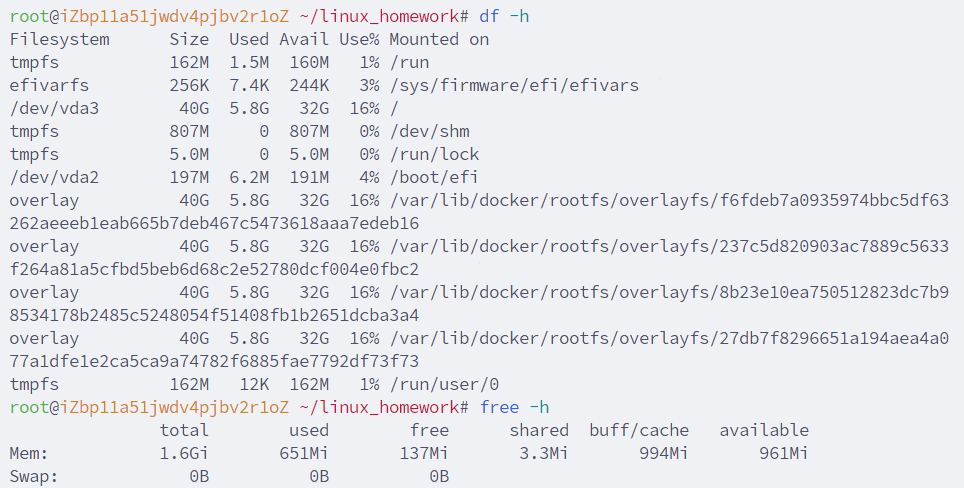
\includegraphics[width=0.8\textwidth]{pic/task1/image copy 7.png}
    \caption{命令3.5-3.6}
\end{figure}

\item 查看系统进程和资源占用：\cmd{top}

\begin{figure}[H]
    \centering
    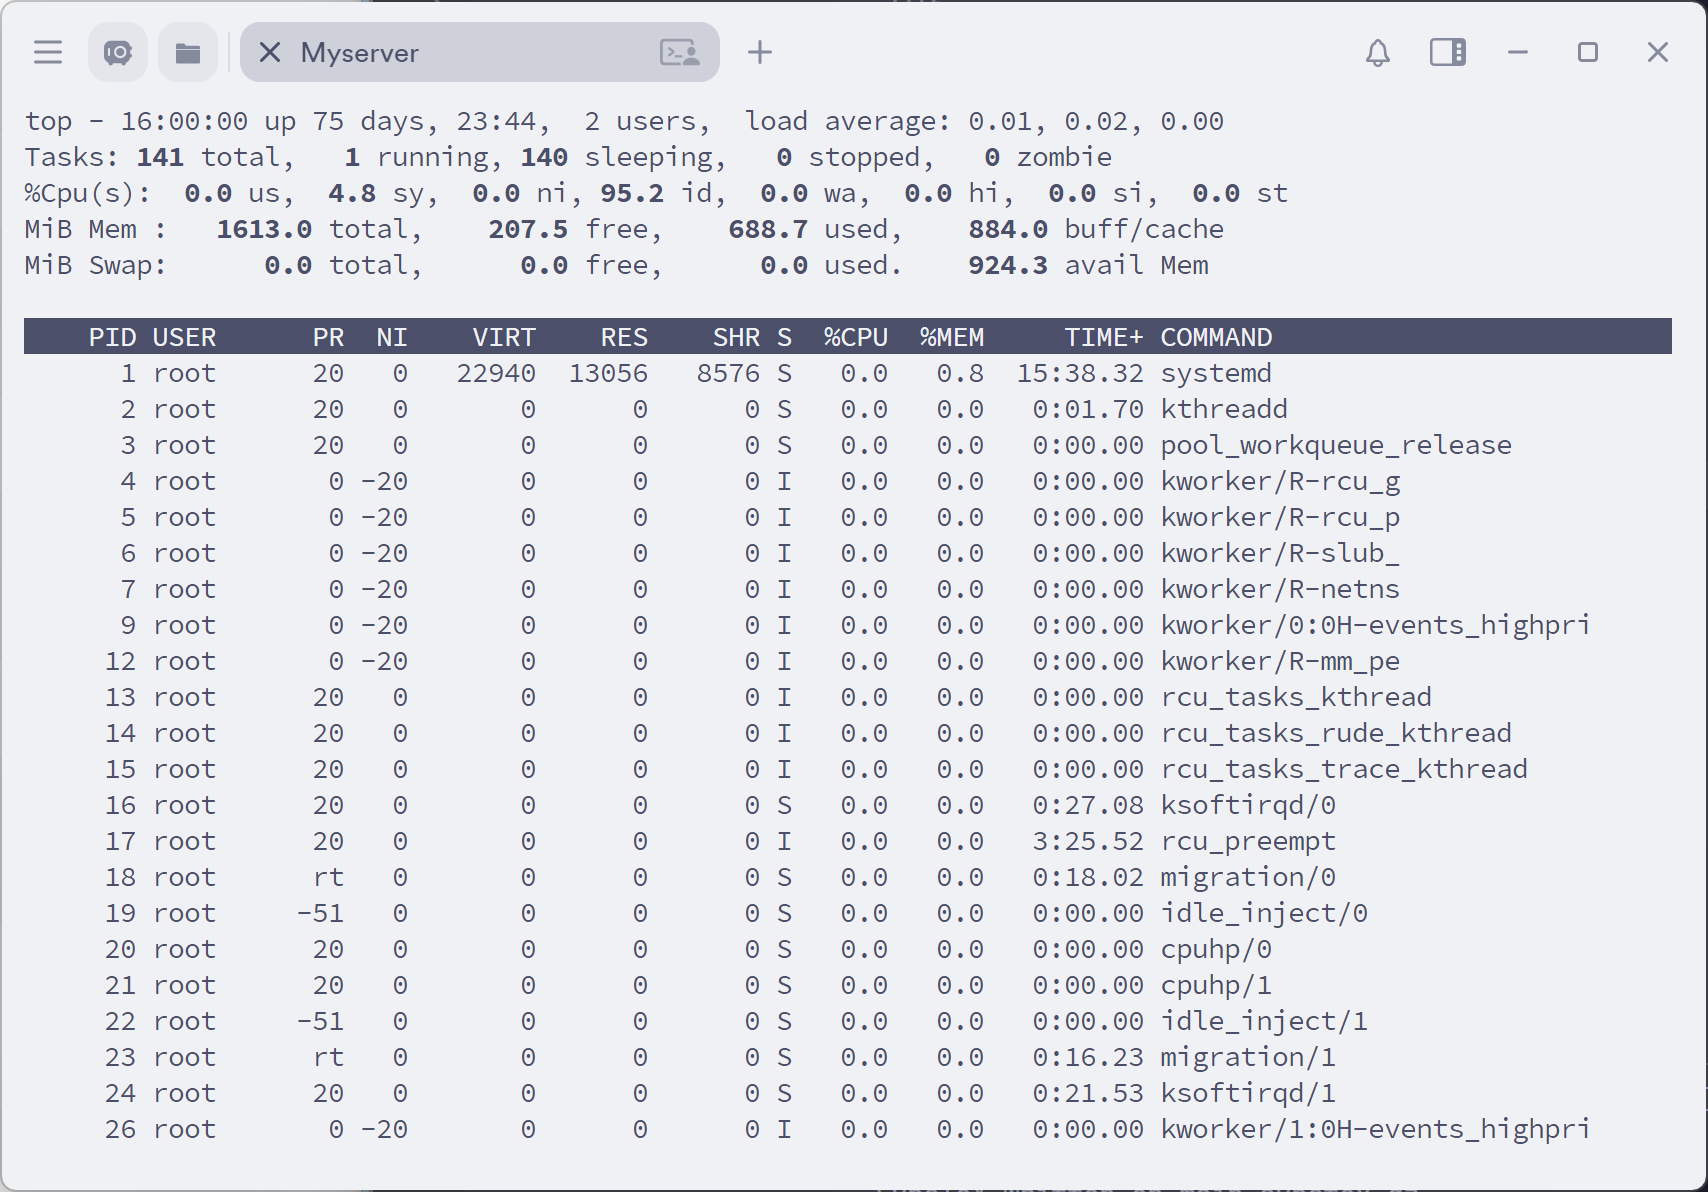
\includegraphics[width=0.8\textwidth]{pic/task1/image copy 8.png}
    \caption{命令3.7}
\end{figure}

\item 查看当前系统进程：\cmd{ps aux}

\begin{figure}[H]
    \centering
    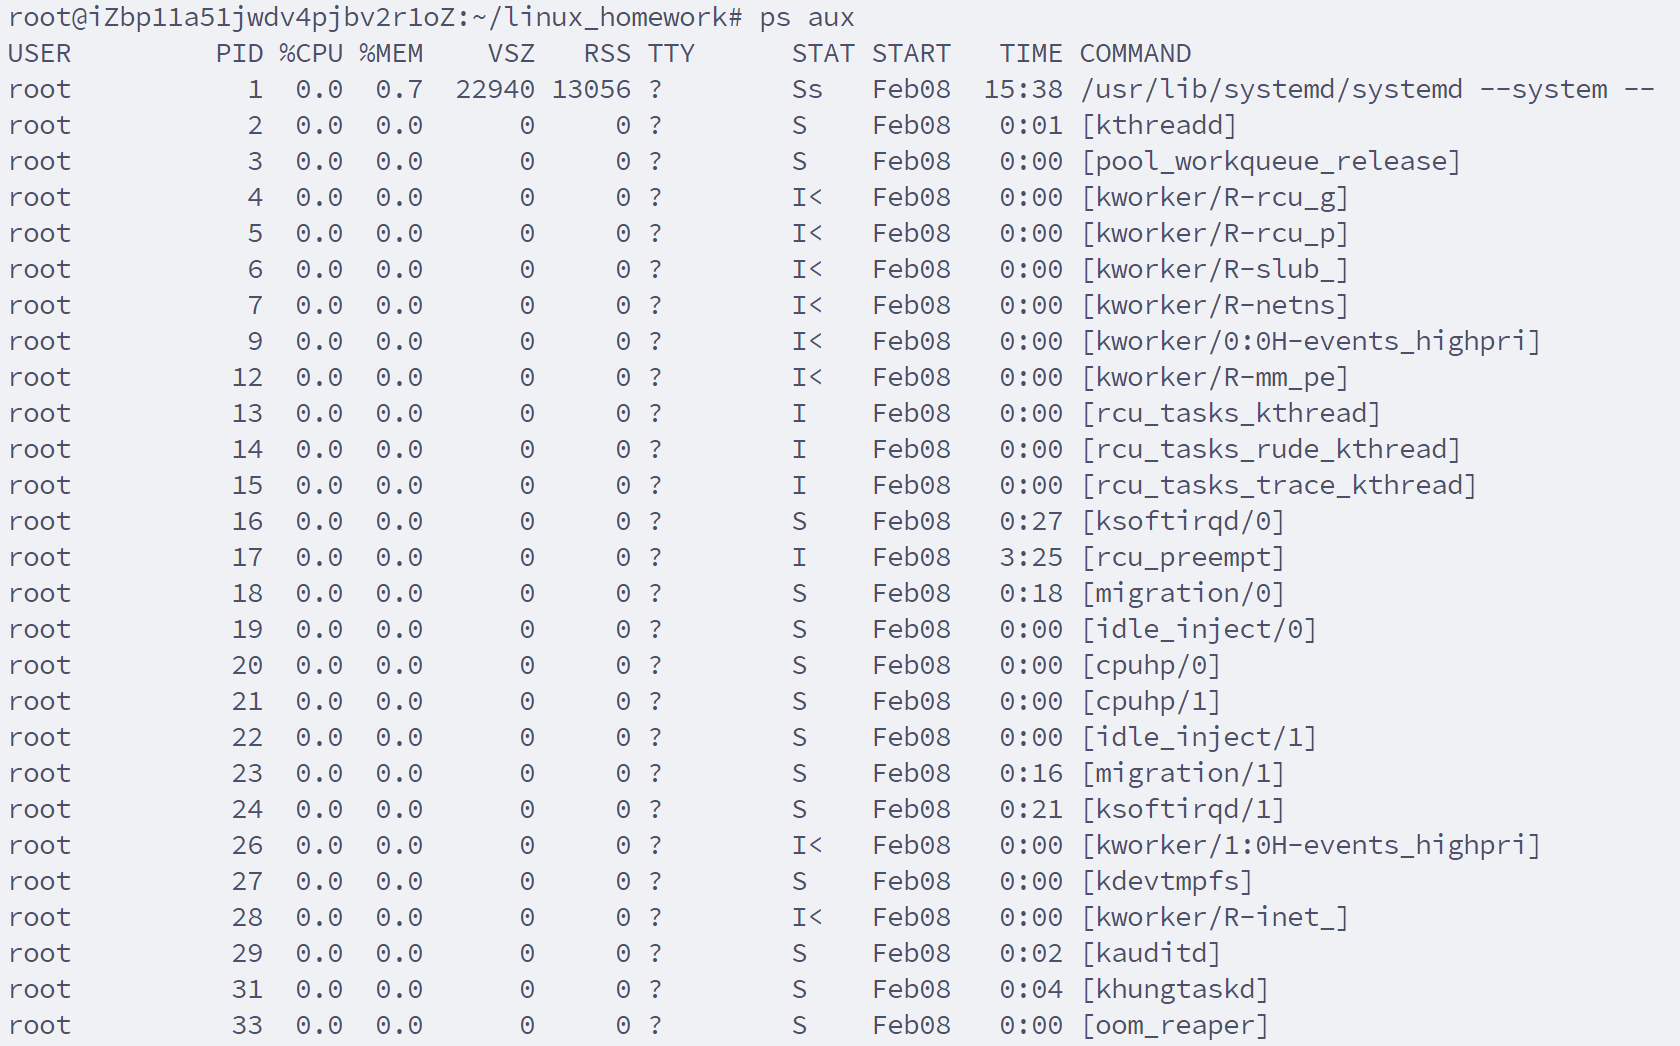
\includegraphics[width=0.8\textwidth]{pic/task1/image copy 9.png}
    \caption{命令3.8}
\end{figure}

由于使用的是远程服务器，系统进程比较多，截图中只保留了与本次演示相关的部分。

\item 查看历史命令：\cmd{history}

\begin{figure}[H]
    \centering
    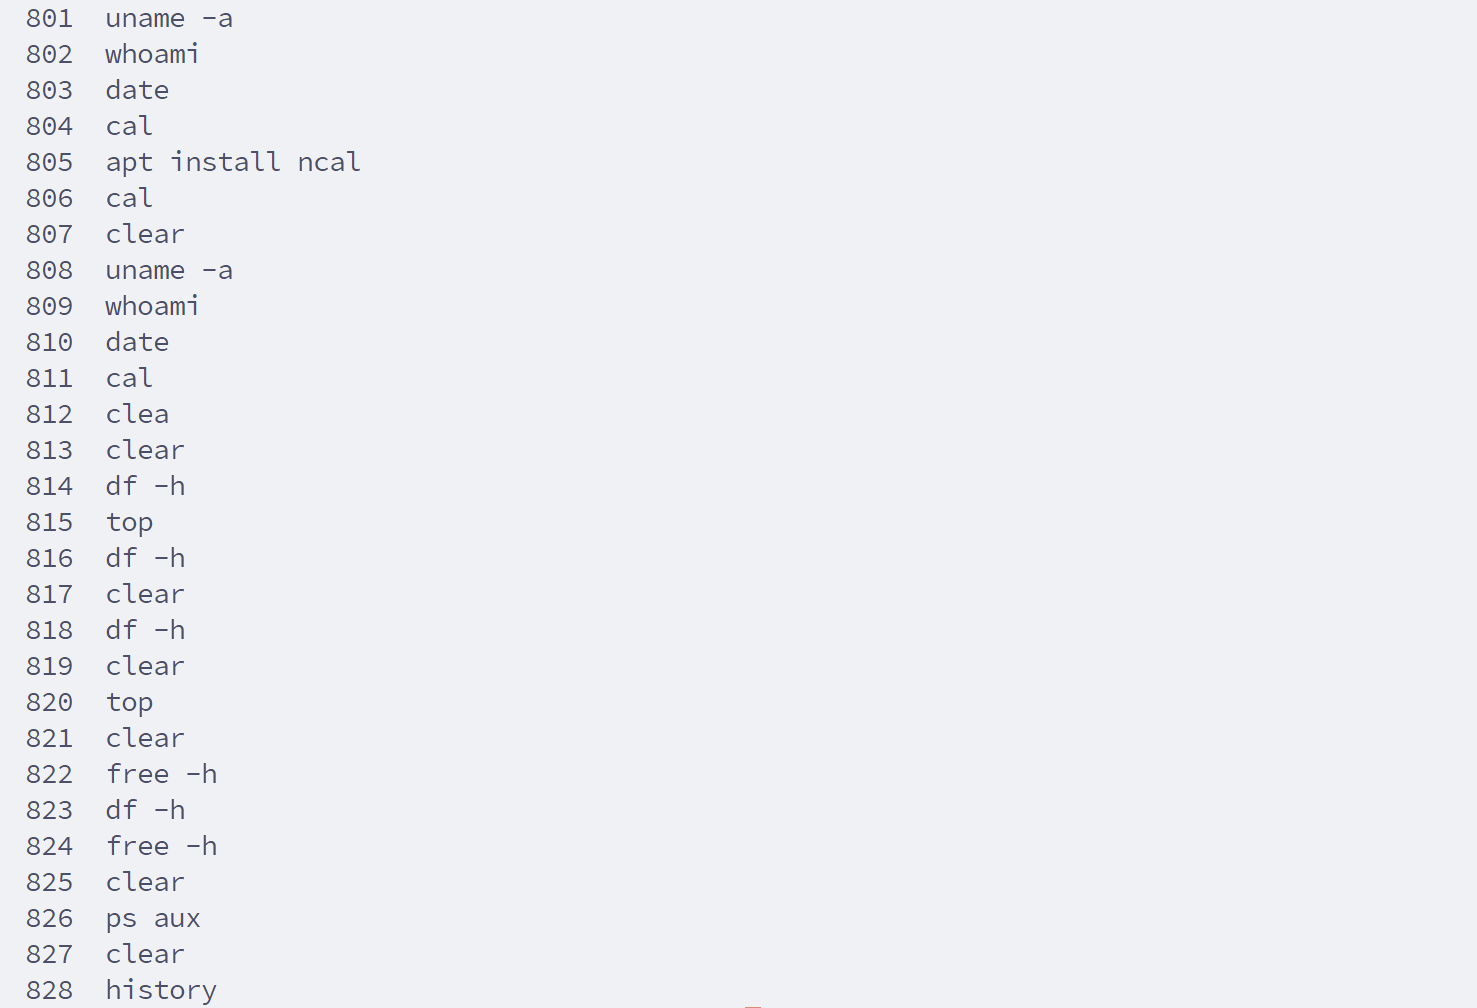
\includegraphics[width=0.8\textwidth]{pic/task1/image copy 10.png}
    \caption{命令3.9}
\end{figure}

历史记录中包含了我之前使用过的命令，包括一些测试命令和安装命令等。这里只截了本次课程展示的几个历史命令。

\end{enumerate}

系统信息命令的作用是帮助使用者判断“当前机器是什么状态”。例如 \cmd{df -h} 可以查看磁盘是否快满，\cmd{free -h} 可以查看内存余量，\cmd{ps aux} 和 \cmd{top} 可以观察进程数量和资源占用。对于服务器实验而言，这些命令尤其重要，因为远程环境没有图形化资源监视器，很多问题都需要通过命令行定位。

\begin{table}[H]
    \centering
    \caption{系统信息命令观察重点}
    \small
    \begin{tabular}{p{0.18\textwidth} p{0.30\textwidth} p{0.34\textwidth}}
        \toprule
        命令 & 主要观察对象 & 使用意义 \\
        \midrule
        \cmd{uname -a} & 内核版本、系统架构和主机信息 & 确认实验环境是否为目标 Linux 系统 \\
        \cmd{whoami} & 当前登录用户 & 判断是否拥有执行某些操作的权限 \\
        \cmd{date} & 当前系统时间 & 配合日志分析命令执行时间 \\
        \cmd{df -h} & 磁盘挂载点和空间使用 & 判断文件写入或编译失败是否与磁盘空间有关 \\
        \cmd{free -h} & 内存和交换空间使用 & 观察服务器是否存在内存压力 \\
        \cmd{ps aux} & 当前进程列表 & 查找正在运行的 shell、Python 或其他服务进程 \\
        \cmd{history} & 历史命令记录 & 复盘实验步骤，便于报告整理 \\
        \bottomrule
    \end{tabular}
\end{table}

\subsection{权限相关命令}

\begin{enumerate}
\item 创建脚本文件：\cmd{touch test.sh}
\item 查看文件权限：\cmd{ls -l test.sh}
\item 给文件添加可执行权限：\cmd{chmod +x test.sh}
\item 再次查看权限变化：\cmd{ls -l test.sh}
\item 查看文件详细状态信息：\cmd{stat test.sh}

\begin{figure}[H]
    \centering
    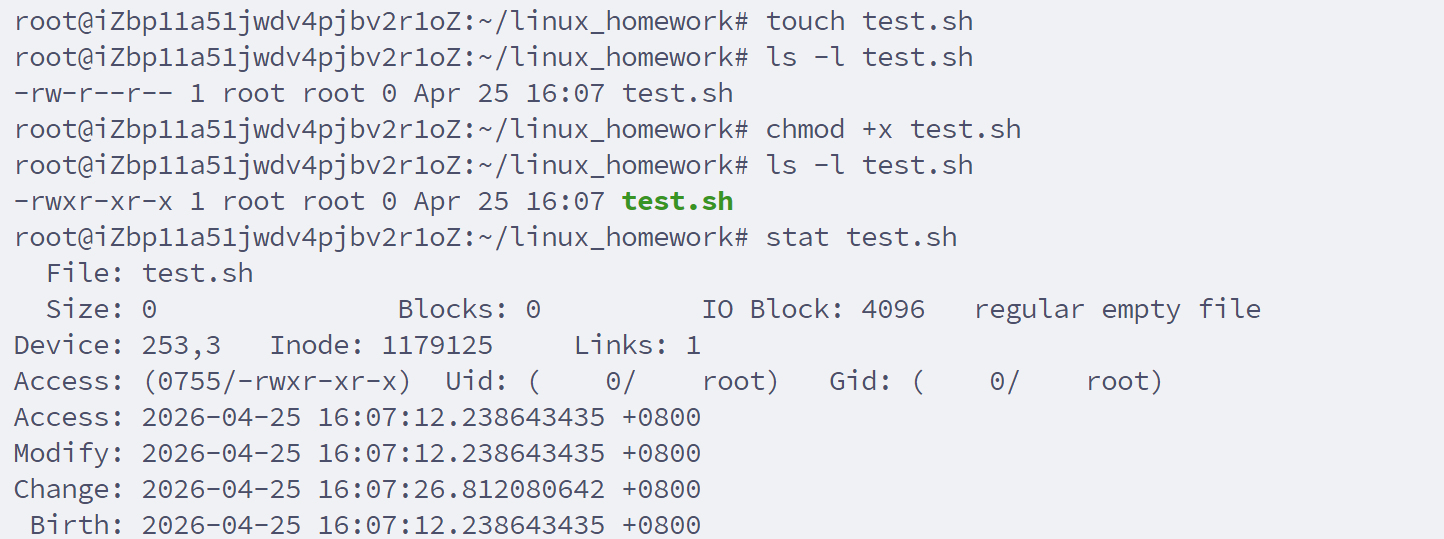
\includegraphics[width=0.8\textwidth]{pic/task1/image copy 11.png}
    \caption{命令4.1-4.5}
\end{figure}

\end{enumerate}

Linux 文件权限通常由三组权限组成，分别对应文件所有者、所属组和其他用户。每一组都可以包含读、写、执行三种权限，显示在 \cmd{ls -l} 输出的前十个字符中。例如普通文件的权限字段可能是 \cmd{-rw-r--r--}，第一个字符表示文件类型，后面九个字符按三组三位展示权限。脚本文件只有添加执行权限后，才可以直接通过 \cmd{./test.sh} 这样的形式运行。

\begin{table}[H]
    \centering
    \caption{权限字符与数字表示}
    \small
    \begin{tabular}{c c c p{0.38\textwidth}}
        \toprule
        权限 & 数字值 & 含义 & 常见影响 \\
        \midrule
        \cmd{r} & 4 & read，读取 & 可以查看文件内容或列出目录内容 \\
        \cmd{w} & 2 & write，写入 & 可以修改文件内容或在目录中创建、删除文件 \\
        \cmd{x} & 1 & execute，执行 & 文件可作为程序运行，目录可被进入 \\
        \cmd{-} & 0 & 无对应权限 & 操作会因权限不足失败 \\
        \bottomrule
    \end{tabular}
\end{table}

数字权限是把同一组中的读、写、执行权限相加得到的。例如 \cmd{7=4+2+1} 表示可读、可写、可执行，\cmd{5=4+1} 表示可读、可执行但不可写，\cmd{4} 表示只读。因此常见的 \cmd{chmod 755 script.sh} 表示所有者拥有全部权限，所属组和其他用户拥有读取与执行权限；\cmd{chmod +x test.sh} 则是在现有权限基础上给文件增加执行权限，更适合本次实验这种只需要让脚本可运行的场景。

\subsection{重定向与错误输出}

除了管道符，重定向也是 Linux 命令行中非常常见的数据流控制方式。管道符把前一个命令的标准输出交给后一个命令，而重定向则把命令的输入或输出连接到文件。本次实验中使用的 \cmd{echo "hello linux" > file1.txt} 就是一个输出重定向例子，它把原本应该显示在终端上的字符串写入文件。

\begin{table}[H]
    \centering
    \caption{常见重定向符号}
    \small
    \begin{tabular}{p{0.18\textwidth} p{0.28\textwidth} p{0.36\textwidth}}
        \toprule
        符号 & 含义 & 示例说明 \\
        \midrule
        \cmd{>} & 覆盖写入标准输出 & \cmd{echo hello > a.txt} 会覆盖原文件内容 \\
        \cmd{>>} & 追加写入标准输出 & \cmd{echo hello >> a.txt} 会把内容追加到文件末尾 \\
        \cmd{<} & 从文件读取标准输入 & 某些命令可以从指定文件中读取输入 \\
        \cmd{2>} & 重定向标准错误 & 把错误信息写入文件，便于排查失败原因 \\
        \cmd{2>\&1} & 将标准错误合并到标准输出 & 常用于同时保存正常输出和错误输出 \\
        \bottomrule
    \end{tabular}
\end{table}

理解标准输出和标准错误的区别，可以帮助定位脚本和命令执行失败的原因。普通结果一般通过标准输出显示，错误提示则通过标准错误显示。很多时候命令看起来“没有输出”，并不代表一定成功；也可能是输出被重定向到了文件，或者错误信息被单独写入了另一个位置。因此在写 Shell 脚本或运行批处理命令时，合理使用重定向可以保留运行记录，也能让后续调试更方便。

\subsection{管道符组合命令}

管道符 | 的作用是将前一个命令的输出结果作为后一个命令的输入。通过管道符，可以把多个简单命令组合成一个更复杂的数据处理流程。例如 \cmd{cat words.txt | sort | uniq -c | sort -nr} 先读取文件内容，再进行排序，然后统计重复行出现次数，最后按照出现次数从高到低排序，体现了 Linux 命令组合使用的灵活性。

\begin{enumerate}
\item 把文件内容传给 sort 排序后去重：\cmd{cat words.txt | sort | uniq}

\begin{figure}[H]
    \centering
    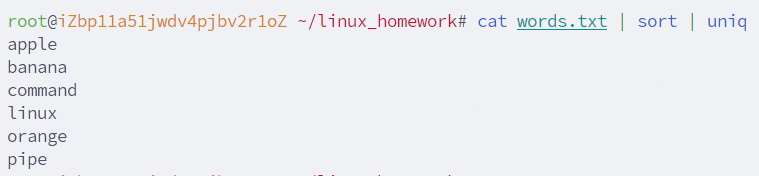
\includegraphics[width=0.8\textwidth]{pic/task1/image copy 12.png}
    \caption{命令5.1}
\end{figure}

\item 统计每个单词出现次数：\cmd{cat words.txt | sort | uniq -c}

\begin{figure}[H]
    \centering
    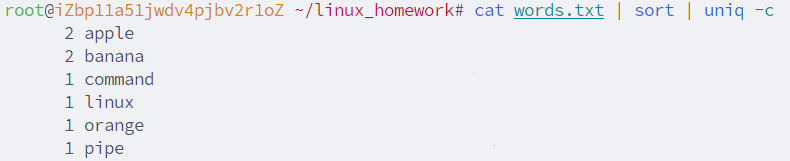
\includegraphics[width=0.8\textwidth]{pic/task1/image copy 13.png}
    \caption{命令5.2}
\end{figure}

\item 找出包含字母 a 的行，并排序：\cmd{grep "a" words.txt | sort}

\begin{figure}[H]
    \centering
    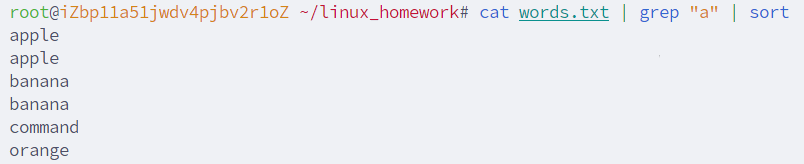
\includegraphics[width=0.8\textwidth]{pic/task1/image copy 14.png}
    \caption{命令5.3}
\end{figure}

\item 在当前目录中筛选 .txt 文件：\cmd{ls | grep '\textbackslash{}.txt\$'}
\item 在进程列表中查找 bash 相关进程：\cmd{ps aux | grep bash}
\item 查看最近使用的命令：\cmd{history | tail}

\begin{figure}[H]
    \centering
    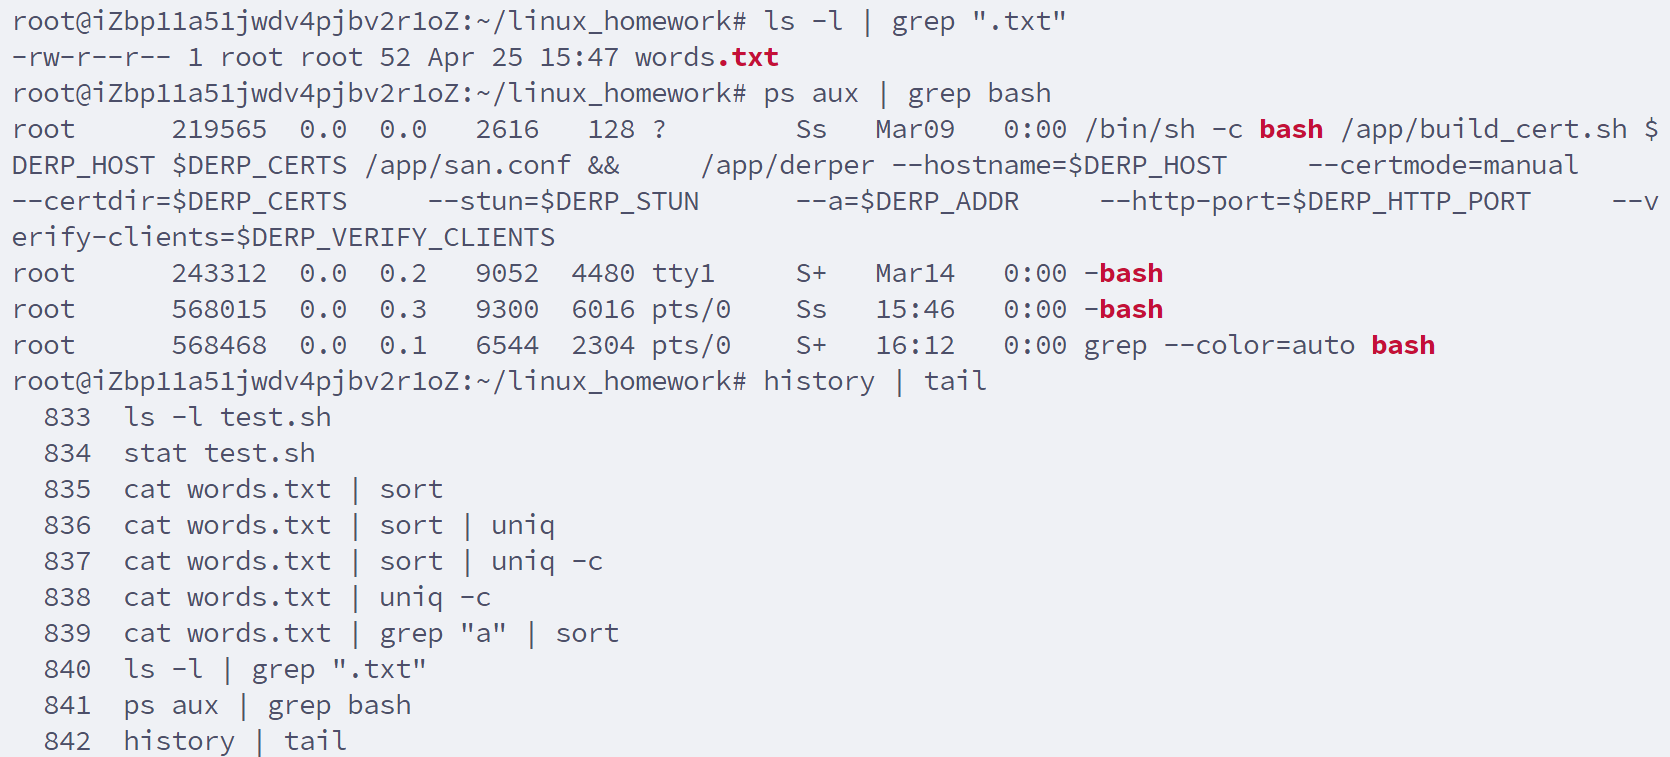
\includegraphics[width=0.8\textwidth]{pic/task1/image copy 15.png}
    \caption{命令5.4-5.6}
\end{figure}

\item 筛选磁盘挂载信息：\cmd{df -h | grep "/dev"}

\begin{figure}[H]
    \centering
    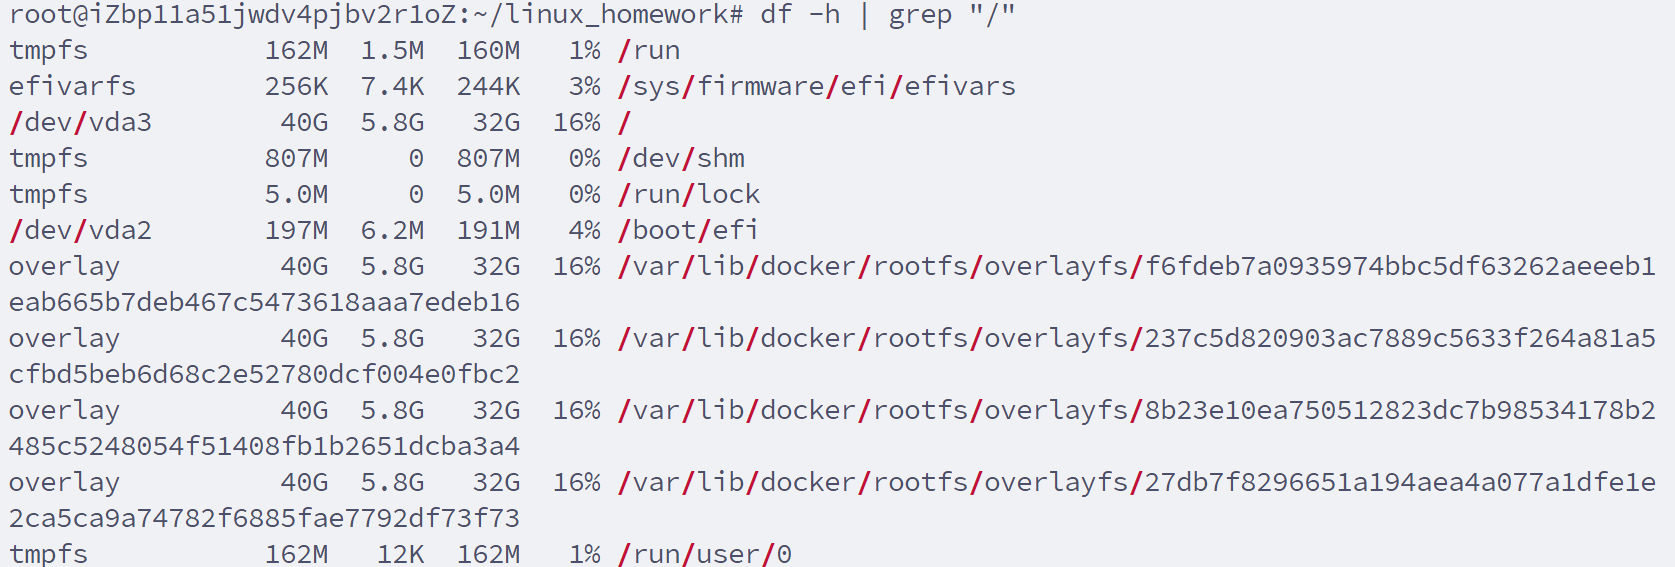
\includegraphics[width=0.8\textwidth]{pic/task1/image copy 16.png}
    \caption{命令5.7}
\end{figure}

\item 统计文件行数：\cmd{cat words.txt | wc -l}
\item 统计单词出现次数，并按出现次数从高到低排序：\cmd{cat words.txt | sort | uniq -c | sort -nr}

\begin{figure}[H]
    \centering
    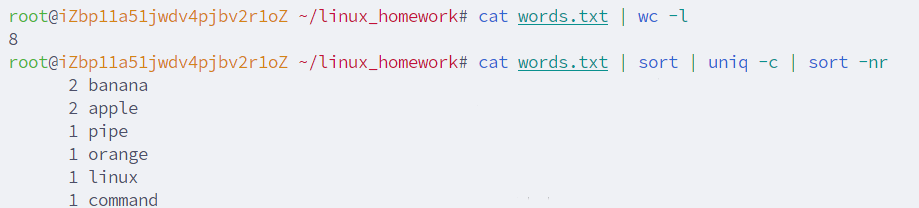
\includegraphics[width=0.8\textwidth]{pic/task1/image copy 17.png}
    \caption{命令5.8-5.9}
\end{figure}

\end{enumerate}

管道命令体现了 Linux 工具设计中的组合思想。每个命令只完成相对单一的任务，例如 \cmd{cat} 负责输出文件，\cmd{sort} 负责排序，\cmd{uniq -c} 负责统计相邻重复项，\cmd{sort -nr} 负责按照数字倒序排列。当这些命令通过管道连接后，就可以完成一个完整的词频统计流程。这种方式比把所有逻辑写进一个大型程序更灵活，也更容易在终端中快速试验。

\begin{table}[H]
    \centering
    \caption{管道组合命令的数据流}
    \small
    \begin{tabular}{p{0.24\textwidth} p{0.30\textwidth} p{0.30\textwidth}}
        \toprule
        命令片段 & 输入 & 输出 \\
        \midrule
        \cmd{cat words.txt} & 文本文件 & 原始单词列表 \\
        \cmd{sort} & 原始单词列表 & 按字典序排列后的行 \\
        \cmd{uniq -c} & 相邻重复内容 & 每个单词及出现次数 \\
        \cmd{sort -nr} & 带计数的行 & 按出现次数从高到低排列的结果 \\
        \cmd{grep "a"} & 多行文本 & 只包含字母 \cmd{a} 的行 \\
        \cmd{wc -l} & 多行文本 & 行数统计结果 \\
        \bottomrule
    \end{tabular}
\end{table}

\subsection{常见命令错误与排查}

在命令行实验中，错误信息本身也是学习内容。Linux 命令通常会明确告诉用户失败原因，例如文件不存在、权限不足、命令未安装或参数错误。遇到错误时，不应该只重新输入命令，而要先判断错误属于路径问题、权限问题、软件包问题还是命令格式问题。

\begin{table}[H]
    \centering
    \caption{常见错误与排查方法}
    \small
    \begin{tabular}{p{0.24\textwidth} p{0.28\textwidth} p{0.32\textwidth}}
        \toprule
        错误现象 & 可能原因 & 排查方法 \\
        \midrule
        \cmd{No such file or directory} & 路径写错或当前目录不对 & 使用 \cmd{pwd} 确认位置，用 \cmd{ls} 查看文件是否存在 \\
        \cmd{Permission denied} & 没有读写或执行权限 & 使用 \cmd{ls -l} 查看权限，必要时使用 \cmd{chmod} 修改 \\
        \cmd{command not found} & 命令未安装或名称拼写错误 & 检查命令拼写，必要时通过包管理器安装 \\
        删除后找不到文件 & \cmd{rm} 已经删除目标 & 删除前先用 \cmd{ls} 确认，重要文件先用 \cmd{cp} 备份 \\
        \cmd{uniq} 去重不完整 & 重复行没有相邻排列 & 先执行 \cmd{sort}，再执行 \cmd{uniq} \\
        管道结果为空 & 前一个命令没有输出或过滤条件太严格 & 分段执行管道，逐步检查每个命令的输出 \\
        \bottomrule
    \end{tabular}
\end{table}

这些排查方法也可以迁移到后面的 Shell 脚本和 Python 项目中。例如脚本无法执行时先看权限，文件读取失败时先看路径，网络服务无法访问时先确认进程是否运行和端口是否开放。命令行学习的价值不只是记住命令本身，更重要的是形成定位问题的顺序。

\subsection{综合命令练习复盘}

把前面几类命令组合起来，可以形成一个完整的小型文本处理任务。例如本次实验中的 \cmd{words.txt} 文件既可以用于查看内容，也可以用于排序、去重、统计和筛选。单独看每条命令时，它们只是简单操作；连起来看时，就能体现 Linux 命令行处理文本数据的能力。

\begin{minted}{bash}
cat words.txt | sort | uniq -c | sort -nr
\end{minted}

这条命令可以拆成四个阶段。第一阶段 \cmd{cat words.txt} 读取文件内容；第二阶段 \cmd{sort} 把相同单词排到相邻位置；第三阶段 \cmd{uniq -c} 统计每个相邻重复项的数量；第四阶段 \cmd{sort -nr} 按数字倒序排列统计结果。每个阶段都只完成一件事，但组合起来就得到了词频统计结果。

\begin{table}[H]
    \centering
    \caption{综合命令执行阶段分析}
    \small
    \begin{tabular}{p{0.18\textwidth} p{0.30\textwidth} p{0.34\textwidth}}
        \toprule
        阶段 & 命令 & 作用 \\
        \midrule
        读取数据 & \cmd{cat words.txt} & 把文本文件内容作为后续命令的数据来源 \\
        排序整理 & \cmd{sort} & 让相同内容相邻，为 \cmd{uniq} 做准备 \\
        统计次数 & \cmd{uniq -c} & 统计每个单词出现次数 \\
        结果排序 & \cmd{sort -nr} & 按出现次数从高到低排列，便于观察高频项 \\
        \bottomrule
    \end{tabular}
\end{table}

这种分阶段思维对后续 Shell 编程也很有帮助。写脚本时不一定要一次写出完整程序，可以先在命令行中把关键命令跑通，再把它们放进变量、循环和函数中。比如第二次作业中的历史成绩统计，本质上也是先读取成绩文件，再使用文本处理命令提取分数字段并计算最高分。

在实际使用中，我也发现管道命令的调试方式与普通程序类似：如果最终结果不对，就把管道从左到右拆开，一段一段执行。先确认原始输入是否正确，再确认排序结果，再确认统计结果，最后再看排序参数是否符合预期。这种调试方法简单但很有效，也体现了 Linux 命令组合的透明性。

\subsection{实验小结}

通过本次基础命令实验，我对 Linux 命令行的工作方式有了更系统的理解。文件和目录命令主要解决“在哪里”和“有什么”的问题，内容查看与处理命令用于观察和整理文本，系统信息命令帮助了解当前运行环境，权限命令则体现了 Linux 中文件可读、可写、可执行权限的基本模型。

其中管道命令给我的印象最深。单个命令的功能通常比较简单，但通过 \cmd{|} 可以把多个命令连接成完整的数据处理流程。例如排序、去重、计数和再次排序可以组合成一条命令完成词频统计。这体现了 Linux 工具“每个程序只做好一件事，再通过组合完成复杂任务”的思想，也为后续 Shell 脚本编程打下了基础。

\newpage

\section{Linux 下的 Shell 编程案例}

本次作业我设计并实现了一个基于 Bash Shell 的 Linux 命令答题系统。程序通过菜单提供开始答题、查看历史成绩、清空历史成绩和退出系统等功能，题目从外部题库文件中读取，答题结束后会把本次成绩保存到成绩文件中。这个案例既能练习 Linux 基础命令，也能体现 Shell 脚本中的条件判断、循环控制、函数封装、文件读写和程序调试等知识点。相比只演示单条命令，答题系统需要把输入、判断、统计、持久化和异常处理组织成完整流程，更能体现 Shell 脚本在 Linux 自动化任务中的作用。

\subsection{程序功能说明}

本程序的主要功能如下：

\begin{itemize}
    \item 显示主菜单，用户可以通过输入编号选择不同功能。
    \item 从 \cmd{questions.txt} 题库文件中逐行读取题目和标准答案。
    \item 判断用户输入是否为空、是否与标准答案一致，并根据结果计算得分和错误次数。
    \item 当答错次数达到设定上限时，系统自动结束本轮答题。
    \item 将每次答题的时间、得分、已答题数和错误题数保存到 \cmd{score.txt} 文件。
    \item 支持查看历史成绩，并使用 \cmd{awk} 统计历史最高分。
    \item 支持清空历史成绩，清空前需要用户再次确认，避免误操作。
\end{itemize}

程序采用“主菜单 + 功能函数”的结构，整体逻辑比较清晰。用户进入程序后，主循环会不断显示菜单，直到用户选择退出。每个功能被封装成独立函数，例如 \cmd{init\_env}、\cmd{show\_menu}、\cmd{start\_quiz}、\cmd{save\_score}、\cmd{show\_history} 和 \cmd{clear\_history}，这样可以减少重复代码。

\subsection{Shell 脚本执行方法}

在 Linux 平台下，可以进入脚本所在目录后执行以下命令运行程序：

\begin{minted}{bash}
cd task2
chmod +x linux_quiz.sh
./linux_quiz.sh
\end{minted}

其中，\cmd{chmod +x linux\_quiz.sh} 用于给脚本添加可执行权限，\cmd{./linux\_quiz.sh} 表示执行当前目录下的脚本文件。

\subsection{程序实现思路}

脚本整体采用函数化结构，把初始化环境、显示菜单、开始答题、保存成绩、查看历史成绩和清空历史成绩拆分为多个函数。主程序只负责循环显示菜单并根据用户选择调用对应函数，这样可以避免所有逻辑堆在一个长脚本中，也方便后续单独修改某个功能。

题库文件使用 \cmd{|} 作为题目和答案之间的分隔符，每一行表示一道题。答题函数通过 \cmd{while IFS='|' read -r question correct\_answer} 逐行读取题库，并使用独立文件描述符读取文件，避免用户输入和题库读取互相干扰。用户输入后，脚本会先去掉首尾空格，再判断是否为空、是否与标准答案一致，并更新分数、已答题数和错误次数。当错误次数达到上限时，当前轮答题自动结束。

成绩文件使用普通文本保存，每条记录包含答题时间、得分、已答题数和错误题数。查看历史成绩时，脚本使用 \cmd{awk} 从成绩文件中统计最高分；清空历史成绩前会要求用户输入确认，避免误删。这样既保持了脚本实现的简单性，也展示了 Shell 脚本对文本文件和命令行工具的组合能力。

\begin{figure}[H]
    \centering
    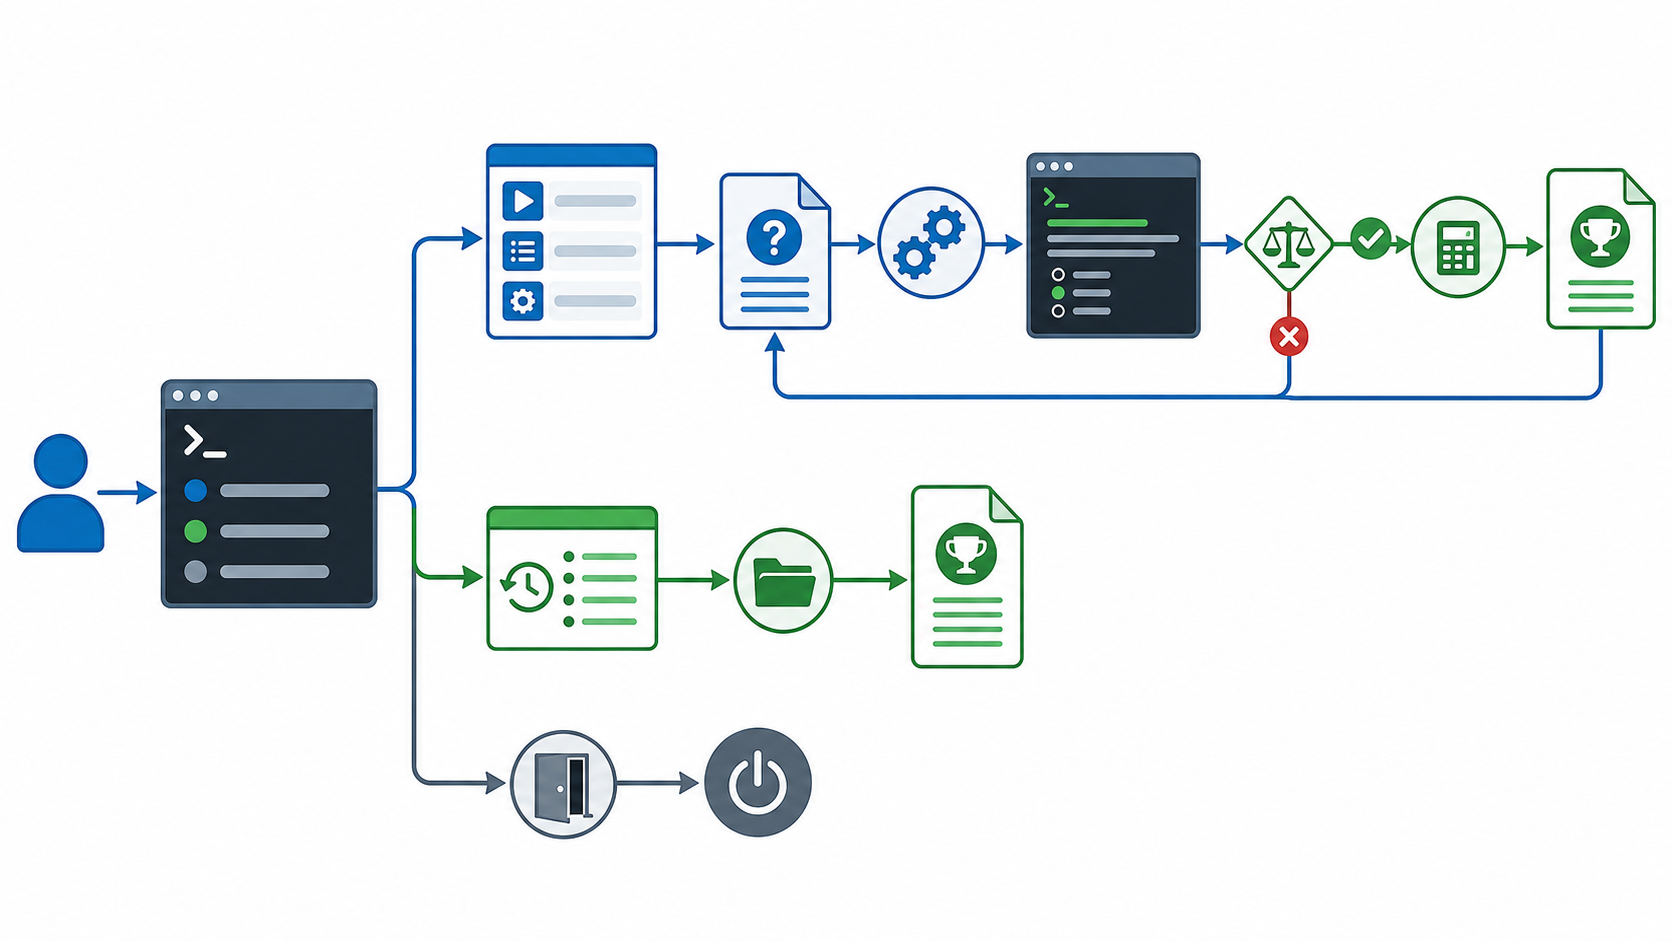
\includegraphics[width=0.85\textwidth]{pic/task2/Shell 答题系统流程图.png}
    \caption{Shell 答题系统流程示意图}
\end{figure}

从流程图可以看出，答题系统不是一次性执行完就退出的线性脚本，而是围绕主菜单形成循环。用户每次输入菜单编号后，脚本通过 \cmd{case} 分支调用对应函数；功能执行结束后再回到菜单，直到用户选择退出。这样的结构比较接近命令行小工具的常见写法，也便于后续继续扩展新功能。

\begin{table}[H]
    \centering
    \caption{Shell 脚本函数职责}
    \small
    \begin{tabular}{p{0.20\textwidth} p{0.34\textwidth} p{0.30\textwidth}}
        \toprule
        函数 & 主要职责 & 涉及的 Shell 知识点 \\
        \midrule
        \cmd{init\_env} & 检查题库文件和成绩文件，准备运行环境 & 文件判断、条件分支、重定向 \\
        \cmd{show\_menu} & 输出主菜单，提示用户选择功能 & \cmd{echo}、终端交互 \\
        \cmd{start\_quiz} & 读取题库、获取用户答案、判断正误、统计分数 & \cmd{while read}、字符串比较、计数变量 \\
        \cmd{save\_score} & 将本次成绩追加到成绩文件 & 输出重定向、日期命令、文本追加 \\
        \cmd{show\_history} & 显示历史成绩并统计最高分 & \cmd{cat}、\cmd{awk}、条件判断 \\
        \cmd{clear\_history} & 二次确认后清空成绩文件 & 用户输入、保护性判断、文件覆盖 \\
        \bottomrule
    \end{tabular}
\end{table}

\begin{table}[H]
    \centering
    \caption{程序文件格式说明}
    \small
    \begin{tabular}{p{0.18\textwidth} p{0.32\textwidth} p{0.34\textwidth}}
        \toprule
        文件 & 格式 & 作用 \\
        \midrule
        \cmd{linux\_quiz.sh} & Bash 脚本文件，包含函数和主循环 & 实现菜单、答题、判分、保存和异常处理 \\
        \cmd{questions.txt} & 每行一题，格式为“题目\cmd{|}答案” & 作为外部题库，便于不改脚本就扩展题目 \\
        \cmd{score.txt} & 每行一条成绩记录，包含时间、得分、题数和错误数 & 保存历史成绩，支持后续查看和统计最高分 \\
        \bottomrule
    \end{tabular}
\end{table}

把题库和成绩从脚本中拆出来，是这个案例中比较重要的设计选择。如果题目直接写在脚本里，每次新增题目都要修改程序逻辑；现在题库作为普通文本文件存在，只要保持分隔符格式一致，就可以继续追加题目。成绩文件同理，它不是复杂数据库，而是适合 Shell 处理的纯文本记录，因此可以直接用 \cmd{cat} 查看，也可以用 \cmd{awk} 做统计。

\subsection{案例展示}

与上一次基础命令作业一致，本次 Shell 脚本也在 Ubuntu 服务器上运行和测试，后续调试同样在这台服务器上完成。

首先创建一个目录来存放本次作业，然后放入 Shell 脚本文件和 \cmd{txt} 题库文件。

\begin{figure}[H]
    \centering
    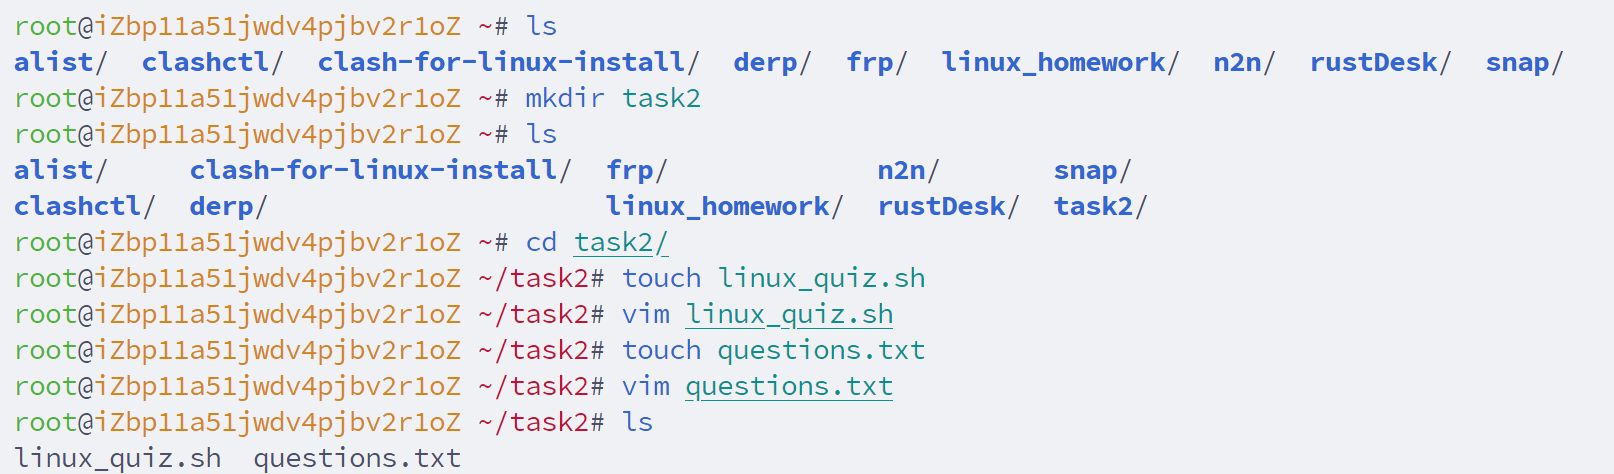
\includegraphics[width=0.8\textwidth]{pic/task2/image.png}
\end{figure}

随后按照前面的执行方法运行脚本。

主菜单页面：

\begin{figure}[H]
    \centering
    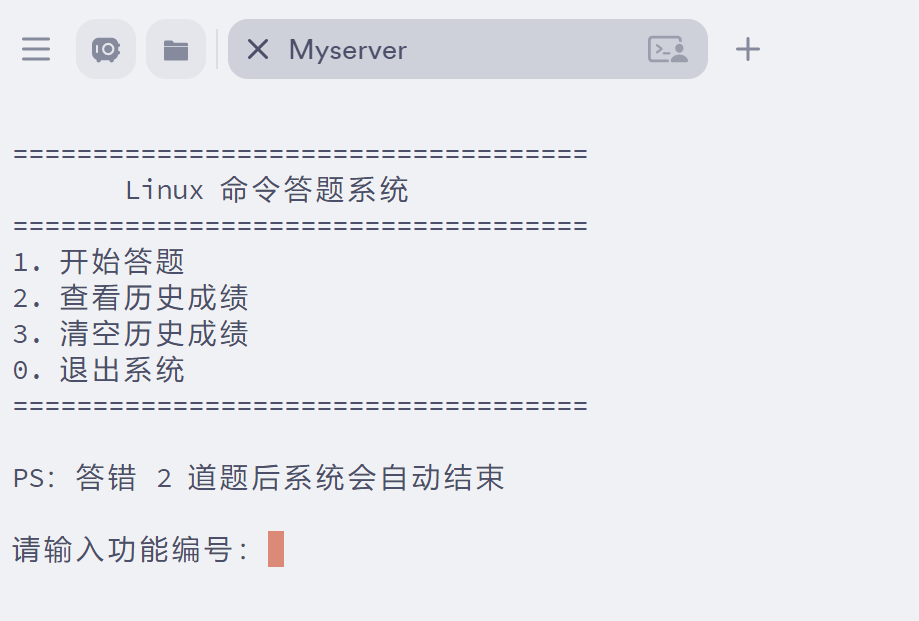
\includegraphics[width=0.8\textwidth]{pic/task2/image copy.png}
\end{figure}

开始答题界面：

\begin{figure}[H]
    \centering
    \begin{minipage}{0.48\textwidth}
        \centering
        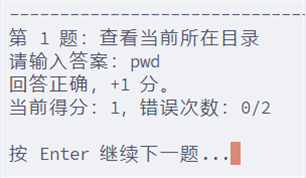
\includegraphics[width=\linewidth]{pic/task2/image copy 3.png}
    \end{minipage}
    \hfill
    \begin{minipage}{0.48\textwidth}
        \centering
        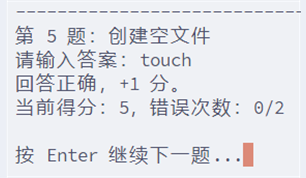
\includegraphics[width=\linewidth]{pic/task2/image copy 4.png}
    \end{minipage}

    \vspace{1em}

    \begin{minipage}{0.48\textwidth}
        \centering
        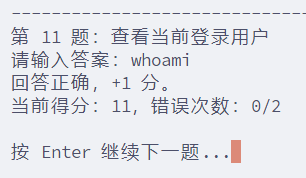
\includegraphics[width=\linewidth]{pic/task2/image copy 5.png}
    \end{minipage}
    \hfill
    \begin{minipage}{0.48\textwidth}
        \centering
        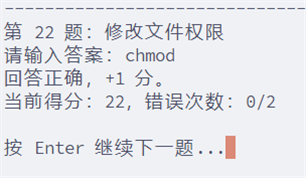
\includegraphics[width=\linewidth]{pic/task2/image copy 6.png}
    \end{minipage}
    \caption{答题界面}
\end{figure}



答题结束界面：

\begin{figure}[H]
    \centering
    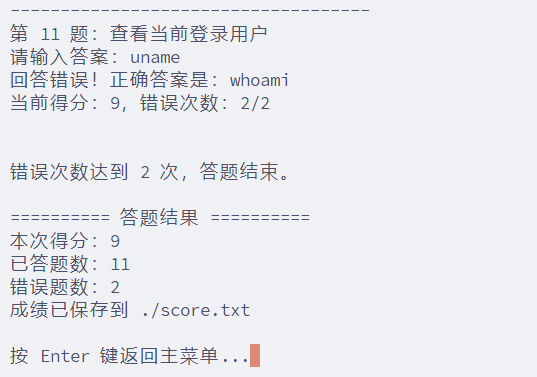
\includegraphics[width=0.8\textwidth]{pic/task2/image copy 2.png}
    \caption{答题结束界面}
\end{figure}

历史成绩界面：

\begin{figure}[H]
    \centering
    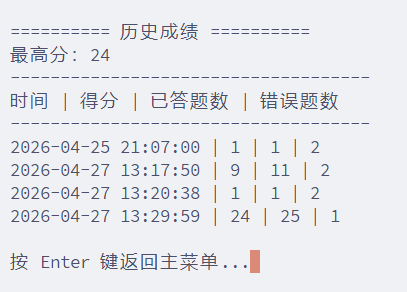
\includegraphics[width=0.8\textwidth]{pic/task2/image copy 7.png}
    \caption{历史成绩}
\end{figure}

题库和历史成绩都保存在当前目录下的 \cmd{txt} 文件中。目前题库包含 25 道题，后续如果需要扩展题库，可以直接在 \cmd{questions.txt} 文件中添加题目和答案，格式为“题目|答案”，每行一题。

\begin{figure}[H]
    \centering
    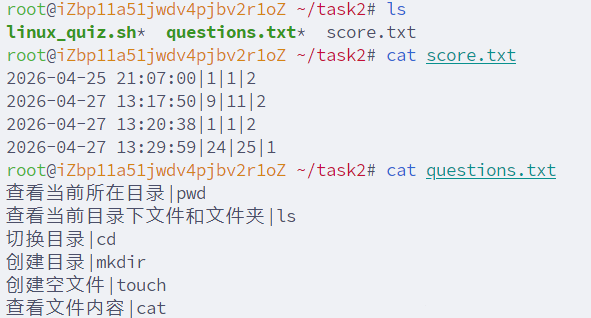
\includegraphics[width=0.8\textwidth]{pic/task2/image copy 8.png}
    \caption{题库和历史成绩文本文件}
\end{figure}

清空历史成绩时，程序会要求用户确认，可以选择确认清空或取消操作。

\begin{figure}[H]
    \centering
    \begin{minipage}{0.48\textwidth}
        \centering
        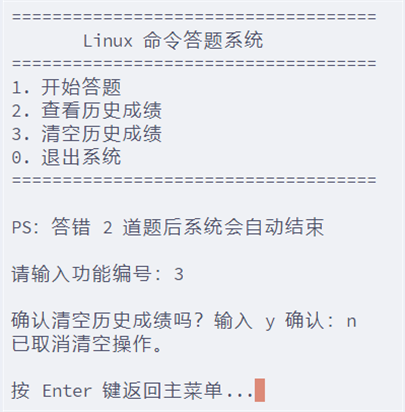
\includegraphics[width=\linewidth]{pic/task2/image copy 9.png}
    \end{minipage}
    \hfill
    \begin{minipage}{0.48\textwidth}
        \centering
        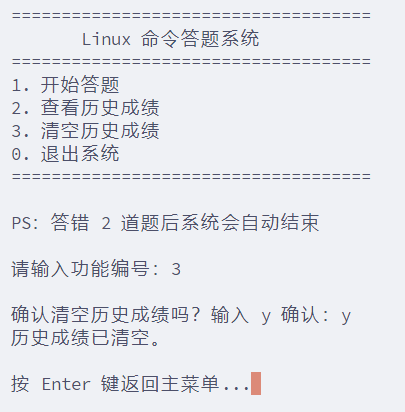
\includegraphics[width=\linewidth]{pic/task2/image copy 10.png}
    \end{minipage}
    \caption{清空历史成绩}
\end{figure}

退出系统。

\begin{figure}[H]
    \centering
    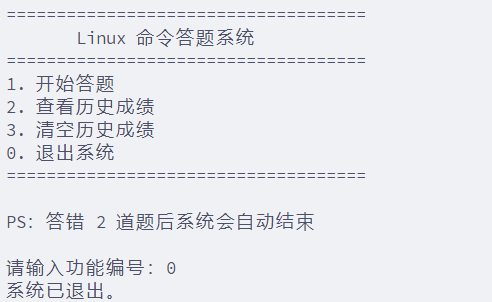
\includegraphics[width=0.8\textwidth]{pic/task2/image copy 11.png}
    \caption{退出系统}
\end{figure}


\subsection{Shell 程序调试方法}

在开发和调试 Shell 脚本时，我主要使用 \cmd{bash -n linux\_quiz.sh} 命令来检查脚本的语法错误。这个命令会解析脚本但不执行它，可以快速发现语法问题。

正常情况下，命令行没有输出，表示没有发现语法错误。

\begin{figure}[H]
    \centering
    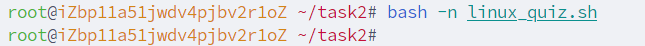
\includegraphics[width=0.8\textwidth]{pic/task2/image copy 12.png}
\end{figure}

如果有错误，会显示错误信息和所在行号，方便定位问题。

\begin{figure}[H]
    \centering
    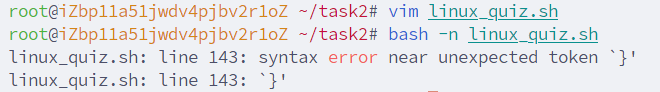
\includegraphics[width=0.8\textwidth]{pic/task2/image copy 13.png}
\end{figure}

使用 \cmd{vim} 打开脚本后可以看到，错误原因是分支结构中少了一个 \cmd{fi}，导致语法检查失败。补全该关键字后再次运行检查，脚本就不再报错。

\begin{figure}[H]
    \centering
    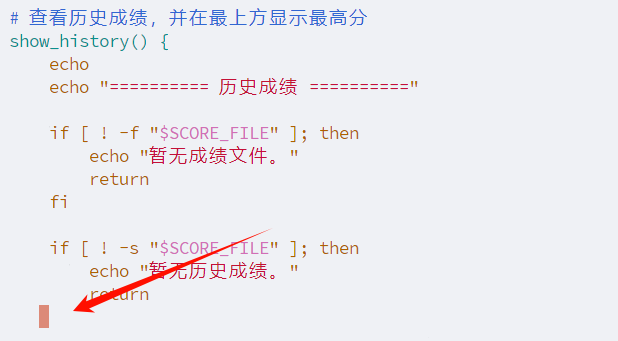
\includegraphics[width=0.8\textwidth]{pic/task2/image copy 14.png}
    \caption{错误修正}
\end{figure}

完成 Shell 脚本之后，可以使用 \cmd{bash -x linux\_quiz.sh} 来执行脚本并显示每条命令的执行过程，这样可以更细致地调试程序逻辑和变量值。

\begin{figure}[H]
    \centering
    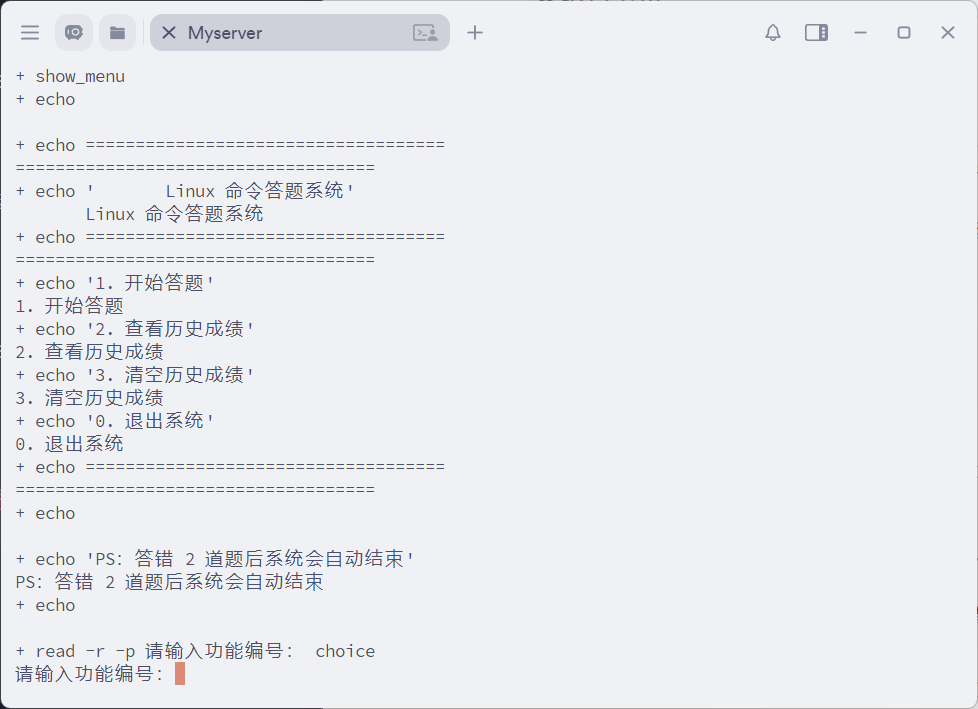
\includegraphics[width=0.8\textwidth]{pic/task2/image copy 15.png}
    \caption{执行跟踪调试}
\end{figure}

另外，我还构造了一些异常输入场景进行测试，例如删除 \cmd{questions.txt}、输入非法选项等，用来验证程序的健壮性和错误处理能力。

删除 \cmd{questions.txt} 后运行程序：

\begin{figure}[H]
    \centering
    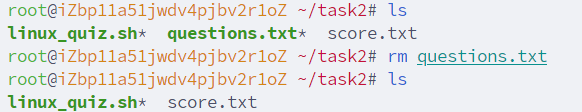
\includegraphics[width=0.8\textwidth]{pic/task2/image copy 16.png}
    \caption{删除题库文件}
\end{figure}

\begin{figure}[H]
    \centering
    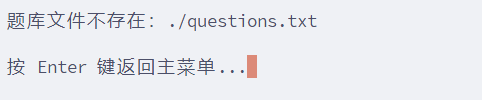
\includegraphics[width=0.8\textwidth]{pic/task2/image copy 17.png}
    \caption{运行程序}
\end{figure}

可以看出程序并没有崩溃，而是提示了题库文件不存在，说明程序的错误处理机制是有效的。

恢复题库文件后，答题输入中文选项：

\begin{figure}[H]
    \centering
    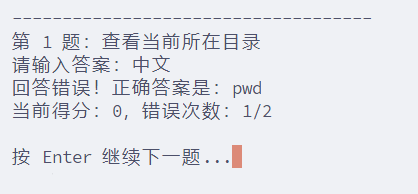
\includegraphics[width=0.8\textwidth]{pic/task2/image copy 18.png}
    \caption{输入中文选项}
\end{figure}

程序能够正确识别并说明该答案错误，说明程序对输入的处理也是正确的。

在主菜单页面输入非法选项时，程序不会崩溃，而是继续循环并提示用户输入正确选项。

\begin{figure}[H]
    \centering
    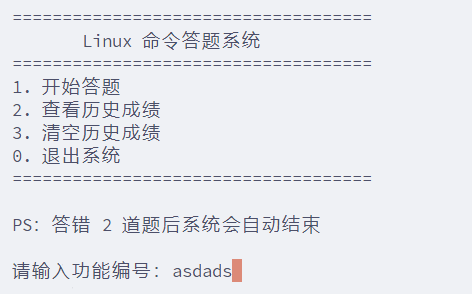
\includegraphics[width=0.8\textwidth]{pic/task2/image copy 19.png}
    \caption{输入非法选项}
\end{figure}

这些异常场景说明，脚本不仅要考虑“用户按预期输入”的情况，还要考虑文件缺失、输入为空、选项非法等常见问题。对于 Shell 程序而言，很多错误都不会自动变成清晰的异常对象，而是表现为命令返回非零状态、变量为空或文件读取失败。因此在关键位置增加文件存在性检查和输入判断，可以显著提高脚本的可用性。

\begin{table}[H]
    \centering
    \caption{异常输入与处理效果}
    \small
    \begin{tabular}{p{0.24\textwidth} p{0.30\textwidth} p{0.30\textwidth}}
        \toprule
        异常场景 & 程序处理方式 & 验证意义 \\
        \midrule
        题库文件缺失 & 输出提示并避免继续读取不存在的文件 & 验证文件检查逻辑有效 \\
        主菜单输入非法编号 & 提示用户重新输入，不退出程序 & 验证 \cmd{case} 默认分支有效 \\
        答题输入中文选项 & 按普通字符串处理并判断为错误答案 & 验证输入读取和字符串比较稳定 \\
        清空成绩前取消确认 & 不删除历史成绩 & 验证危险操作前的二次确认 \\
        成绩文件为空 & 仍能进入历史成绩功能并给出合理提示 & 验证查看历史时的边界情况 \\
        \bottomrule
    \end{tabular}
\end{table}

\subsection{脚本可维护性分析}

从可维护性角度看，这个答题系统虽然规模不大，但已经具备了几个比较好的脚本结构。首先，功能被拆分成多个函数，主循环只负责菜单分发，使脚本入口保持清晰。其次，题库和成绩使用外部文本文件保存，数据和程序逻辑没有混在一起。再次，清空历史成绩这种危险操作加入确认步骤，降低了误操作风险。

如果后续继续扩展，可以优先保持现有的函数化结构。例如增加随机抽题时，可以新增一个题目选择函数；增加错题本时，可以新增一个错题保存文件；增加排行榜时，可以在现有成绩文件基础上使用 \cmd{sort}、\cmd{awk} 等命令统计。这样扩展不会破坏已有菜单，也不需要重写全部答题流程。

\subsection{菜单循环与数据流分析}

这个 Shell 程序的主干是菜单循环。菜单循环的好处是用户可以反复执行不同功能，而不需要每次都重新启动脚本。用户选择开始答题后，程序进入答题流程；选择查看历史成绩后，程序读取成绩文件；选择清空历史成绩后，程序先确认再清空；选择退出后，循环结束。

\begin{table}[H]
    \centering
    \caption{菜单选项与数据流}
    \small
    \begin{tabular}{p{0.18\textwidth} p{0.28\textwidth} p{0.36\textwidth}}
        \toprule
        菜单选项 & 读取的数据 & 写入或输出的结果 \\
        \midrule
        开始答题 & \cmd{questions.txt} 中的题目和答案 & 在终端显示题目，结束后把成绩写入 \cmd{score.txt} \\
        查看历史成绩 & \cmd{score.txt} 中的历史记录 & 在终端输出历史记录，并统计最高分 \\
        清空历史成绩 & 用户确认输入 & 覆盖或清空 \cmd{score.txt}，删除历史记录内容 \\
        退出系统 & 用户菜单选择 & 结束主循环，脚本正常退出 \\
        \bottomrule
    \end{tabular}
\end{table}

从数据流角度看，题库文件是输入数据，成绩文件是输出数据，终端既是输入界面也是输出界面。用户通过 \cmd{read} 输入菜单编号和答案，脚本通过条件判断和循环控制决定下一步操作。这个结构虽然简单，但已经包含了交互式命令行程序的基本要素。

答题流程内部还有一层循环：外层菜单循环控制功能选择，内层题目循环逐行读取题库。内层循环每读到一行，就把分隔符左边作为题目，右边作为标准答案。用户输入答案后，脚本更新得分、已答题数量和错误次数。如果错误次数达到上限，内层循环提前结束，然后把本轮结果保存到成绩文件。


通过这个案例可以看到，Shell 脚本并不只适合写一两条自动化命令，也可以组织成有状态的交互程序。只要把数据文件、变量、循环和函数设计清楚，Shell 就能够完成比较完整的命令行应用。它的优势是直接利用 Linux 自带命令和文本文件，缺点是复杂数据结构和大型界面不如通用编程语言方便。

\subsection{实验小结}

这个 Shell 编程案例把前一节学到的基础命令进一步组织成了一个可交互的小程序。脚本中既有 \cmd{read} 获取用户输入，也有 \cmd{if} 和 \cmd{case} 完成分支判断，还有 \cmd{while} 循环读取题库文件，并通过重定向把成绩追加到文本文件中。相比单独练习命令，完整脚本更强调流程设计和异常处理。

通过调试过程可以看到，Shell 脚本虽然语法相对简洁，但对符号和结构非常敏感，例如缺少 \cmd{fi} 就会导致语法检查失败。因此在编写脚本时，先用 \cmd{bash -n} 检查语法，再用 \cmd{bash -x} 跟踪执行过程，是比较实用的调试方法。后续如果继续完善这个答题系统，还可以增加随机出题、错题记录、分数排行榜和题库合法性检查等功能。

\subsection{源代码与题库展示}

以下是本次 Shell 编程作业的主要源代码和配套题库文件。其中，\cmd{linux\_quiz.sh} 负责菜单交互、答题流程、成绩保存和异常处理，\cmd{questions.txt} 则保存题目与标准答案。题库文件采用“题目|答案”的格式组织，每行对应一道题。题库文件可以根据需要进行扩展，添加更多题目和答案。

\subsubsection{Shell 脚本}

\inputminted{bash}{code/task2/linux_quiz.sh}

\subsubsection{题库文件}

\inputminted{text}{code/task2/questions.txt}




\end{document}
